\RequirePackage[l2tabu, orthodox]{nag}		%checks for obsolete LaTeX packages and outdated commands
\documentclass[
	fontsize=11pt,%				Schriftgroesse 11pt
	paper=a4,%					Layout fuer Din A4
	twoside=false,%				Layout fuer beidseitigen Druck %semi %true
	twocolumn=false,%			zweispaltiger Satz
	headsepline=true,%			horizontale Linie unter Kolumnentitel
	footsepline=false,%			Trennline zum Seitenfuß
	headinclude=true,%			Kopfzeile wird Seiten-Layouts mit beruecksichtigt
	footinclude=false,%			Fußzeile wird Seiten-Layouts mit beruecksichtigt
	chapterentrydots=false,%	Inhaltsverzeichnis dotfill für Kapitel
	parskip=false,%				Der erste Absatz eines Abschnitts wird nicht eingezogen
	BCOR=12mm,%					Korrektur fuer die Bindung
	DIV=15,%					DIV-Wert fuer die Erstellung des Satzspiegels, siehe scrguide	%calc
	parskip=half,%				Absatzabstand statt Absatzeinzug
	footnotes=multiple,%		Fußnotenmarkierungen %nomultiple
	headings=openany,%			Kapitel können auf geraden und ungeraden Seiten beginnen %openleft %openright
	index=default,%				Index im Inhaltsverzeichnis %totoc %numbered
	bibliography=totoc,%		Literaturverz. Wird ins Inhaltsverzeichnis eingetragen
	listof=totoc,%				Tabellen und Abbildungs. Wird ins Inhaltsverzeichnis eingetragen
	numbers=noendperiod,%		Kapitelnummern immer ohne Punkt	%endperiod %autoendperiod
	draft=false,%				Keine Bilder in der Anzeige, overfull hboxes werden angezeigt
	titlepage=true,%			Titlei auf erster Seite	%firstiscover
	chapterprefix=false,%		Kapitelprefix für mainmatter
	appendixprefix=true,%		Kapitelprefix für Anhang
	bibliography=oldstyle,%		Formatierungsstil des Literaturverzeichnisses %openstyle
	cleardoublepage=plain,%		Leere seiten plain
	pagesize=auto,%				Ausgabetreiber %pdftex
	]{scrbook}%					crbook 2018/01/23 v3.24

\usepackage{scrhack}
\usepackage{scrwfile}
\usepackage{ifluatex}
\usepackage{siunitx}   %einheit


\usepackage[english, ngerman]{babel}%		Nötig, damit Dokument in Deutsch generiert wird
\usepackage[utf8]{luainputenc}%				Nötig um Umlaute zu tippen. Alternativ: latin1
\ifluatex
	\usepackage[no-math]{fontspec}
\else
	\usepackage[T1]{fontenc}%				font encoding
\fi

\usepackage[centertags]{amsmath}%	AMS-Mathematik, %centertags zentriert Nummer bei split, %fleqn
\interdisplaylinepenalty=2500
\usepackage{amsthm}
\usepackage{amsfonts}%				Standard fonts
\usepackage{amssymb}%				Standard fonts
\usepackage{gensymb}
\usepackage{array}
\usepackage{mathtools}%				Multiline and split equations
\usepackage{relsize}
\usepackage{physics}

%\usepackage{graphicx}
%\DeclareGraphicsExtensions{.tif,.jpg,.pdf,.mps,.png} 
\ifluatex
	\usepackage[luatex]{graphicx}%			Package um grafiken zu includieren
\else
	\usepackage[pdftex]{graphicx}%
\fi
\usepackage{textcomp}%						verschiedene Symbole
\usepackage[onehalfspacing]{setspace}%		Zeilenabstand anpassen
	\KOMAoptions{DIV=last}%					Seitenspiegel durch setspace nicht verändern
\usepackage{float}
\usepackage[hang, bf, font=small, textformat=period]{caption}%	Captions für s und tables
\usepackage{subcaption}%					Package um subfigure zu erstellen
\usepackage[svgnames, table]{xcolor}%		Farbkonversion etc.
\usepackage{colortbl}%						Support for colors in tables
\usepackage{multirow}%						Zelle einer Tabelle über mehrere Zeilen ausdehnen
\usepackage{array}
\usepackage{makecell}
\usepackage{booktabs}%						Tabellenformatierung
\usepackage{rotating}%						Rotation von tables und figures
\usepackage{tikz}%							Zeichnen direkt in Latex
\usepackage[siunitx]{circuitikz}%			Zeichnen von elektrischen Schaltbildern direkt in Latex
\usepackage{pgfplots}
	\pgfplotsset{
		compat=newest,%						% TODO: set to current version of pgfplots, when starting your work (2018/01/23: compat=1.15)
		width=0.8\textwidth,%
		colormap={blackwhite}{gray(0cm)=(0); gray(1cm)=(1)},%
	}
\usepackage{siunitx}
	\sisetup{
		locale = DE,%
		detect-all,%
% 		scientific-notation = engineering,%
		list-final-separator = { und },%
		list-pair-separator = { und },%
		range-phrase = { bis },%
		per-mode = symbol,%
		binary-units = true,%
		quotient-mode = fraction,%
		output-complex-root = j,%
	}
	\DeclareSIUnit[]\dBm{dBm}
	\DeclareSIUnit[]\dBW{dBW}
\usepackage{calc}%							Hilfspaket um mit Latex variablen zu rechnen
\usepackage{listings}%						Paket um sourcecode zu publizieren

\lstnewenvironment{matlab}[1][]{
	\lstset{
		backgroundcolor=\color{white}, %\color{TUgreen!20}, %\color{gray!20}
		fillcolor=,% %\color{black},
		captionpos=t,% b
		tabsize=4,%
		rulecolor=\color{black},%
		rulesepcolor=\color{gray!30},%
		language=Matlab,%
		basicstyle=\small,%
		numbers=left,%
		numberfirstline=true,%
		numberblanklines=true,%
		stepnumber=1,%
		numbersep=5pt,%
		numberstyle=\scriptsize,%
		upquote=true,%
		aboveskip={0\baselineskip},%
% 		belowskip=\baselineskip,%
		columns=flexible,% %fixed,
		showstringspaces=false,%
		extendedchars=true,%
		breaklines=true,%
		breakatwhitespace=true,%
		prebreak = \raisebox{0ex}[0ex][0ex]{\ensuremath{\color{black}\hookleftarrow}},%
		breakautoindent=true,%
		frame=single,% %tblr, %shadowbox, %tblrTBLR,
		frameround=ffff,% %tttt,
		showtabs=false,%
		showspaces=false,%
		showstringspaces=false,%
		identifierstyle=\ttfamily,%
		basicstyle=\ttfamily\color{black},%
		keywordstyle=\ttfamily\bfseries\color{MidnightBlue},%
		commentstyle=\color{tudark},% %\color{MediumTurquoise},
		stringstyle=\color{DarkOrchid},%
		mathescape=true,%
		showlines=true,%
		escapechar=§,%							escape to latex
		abovecaptionskip=0\smallskipamount,%
		belowcaptionskip=3\smallskipamount,%
		xleftmargin=1.25\baselineskip,%
		xrightmargin=0pt,
		#1,%									add more options from the optional parameter
	}}{}
\usepackage[
	pdfpagelabels,
	colorlinks=false,
	plainpages=false,
	pdfborder={0 0 0},
	]{hyperref}%						Automatische Kreuzreferenzierungen (auch URLs) im PDF
\makeatletter
\AtBeginDocument{\hypersetup{
		pdftitle = {\@documentnumber},%
		pdfsubject = {\@title},%
		pdfauthor = {\@author},%
		pdfkeywords = {},%
		bookmarksopen = {true},%
		bookmarksdepth = 3,%			up to subsubsection titles will be included into PDF structure
		bookmarksopenlevel = 1,%		... up to section titles
	}
}
\usepackage[acronym,nonumberlist,section=chapter,translate=false,shortcuts,toc=true]{glossaries} % Glossar, Abkürzungsverzeichniss etc.
	\renewcommand{\acronymname}{Abkürzungsverzeichnis}
	\newglossary[slg]{symbol}{sym}{sbl}{Symbolverzeichnis}
	\makeglossaries
	\newglossarystyle{tab_style}{
		\renewenvironment{theglossary}{\begin{longtable}[l]{llp{0mm}}}{\end{longtable}}
		\renewcommand*{\glsgroupheading}[1]{}
		\renewcommand*{\glossentry}[2]{\glsentryitem{##1}\glstarget{##1}{\textbf{\glossentryname{##1}}} & \glossentrydesc{##1} & ##2 \tabularnewline[3px]}
		\renewcommand*{\subglossentry}[3]{\glossentry{##2}{##3}}
		\renewcommand*{\glsgroupskip}{}
	}
	\newglossarystyle{tab_style_sym}{ 
		\renewenvironment{theglossary}{\begin{longtable}[l]{llp{0mm}}}{\end{longtable}}
		\renewcommand*{\glsgroupheading}[1]{}
		\renewcommand*{\glossentry}[2]{\glsentryitem{##1}\glstarget{##1}{\glossentrysymbol{##1}} & \glossentrydesc{##1} & ##2 \tabularnewline[3px]}
		\renewcommand*{\subglossentry}[3]{\glossentry{##2}{##3}}
		\renewcommand*{\glsgroupskip}{}
	}

%%% Symbols
%
\newglossaryentry{pi}{type=symbol,name=\ensuremath{\pi},symbol={\ensuremath{\pi}},sort=pi,description={ratio of circumference of circle to its diameter}}
\newglossaryentry{ohm}{type=symbol,name=ohm,symbol={\ensuremath{\Omega}},description=unit of electrical resistance}
\newglossaryentry{angstrom}{type=symbol,name={\aa}ngström,symbol={\AA},sort=angstrom,description={non-SI unit of length}}
\newglossaryentry{angstro}{type=symbol,name=angstrom,symbol={A},description=non-SI unit of length}


%%% Acronyms

\newacronym{vlc}{VLC}{\textbf{V}isible \textbf{L}ight \textbf{C}ommunication}
\newacronym{david}{DaVid}{\textbf{Da}ta transmission using \textbf{Vi}deo \textbf{d}evices}
\newacronym{surf}{SURF}{\textbf{S}peeded \textbf{U}p \textbf{R}obust \textbf{F}eatures}
\newacronym{sift}{SIFT}{\textbf{S}cale \textbf{I}nvariant \textbf{F}eature \textbf{T}ransform}
\newacronym{ransac}{RANSAC}{\textbf{RAN}dom \textbf{SA}mple \textbf{C}onsensus}
\newacronym{ncc}{NCC}{\textbf{N}ormalized \textbf{C}ross \textbf{C}orrelation}


\newacronym{led}{LED}{\textbf{L}ight-\textbf{E}mitting \textbf{D}iode}
\newacronym{ieee}{IEEE}{\textbf{I}nstitute of \textbf{E}lectrical and \textbf{E}lectronics \textbf{E}ngineers}
\newacronym{abc}{abc}{test}
\newacronym{HDTV}{HDTV}{\textbf{h}igh \textbf{d}efinition \textbf{t}ele\textbf{v}ision}
\newacronym{ISI}{ISI}{inter symbol interference}
\newacronym{gpu}{GPU}{\textbf{G}raphics \textbf{P}rocessing \textbf{U}nit}
\newacronym{eeprom}{EEPROM}{electrically erasable programmable read-only memory}%	load symbol and acronym defintions
\glsaddallunused[\acronymtype]%				add all abbreviations
\glsaddallunused[symbol]%					add all symbols
\makeatother

% *** CITATION PACKAGES ***
\usepackage[style=ieee, backref=false, dashed=false, doi=false, isbn=false, backend=biber]{biblatex}
\usepackage[autostyle=true, german=quotes]{csquotes}
\addbibresource{literatur.bib}

\DeclareBibliographyDriver{standard}{%
	\usebibmacro{bibindex}%
	\usebibmacro{begentry}%
	\usebibmacro{author}%
	\setunit{\labelnamepunct}\newblock
	\usebibmacro{title}%
	\newunit\newblock
	\printfield{number}%
	\setunit{\addspace}\newblock
	\printfield[parens]{type}%
	\newunit\newblock
	\usebibmacro{location+date}%
	\newunit\newblock
	\iftoggle{bbx:url}
		{\usebibmacro{url+urldate}}
		{}%
	\newunit\newblock
	\usebibmacro{addendum+pubstate}%
	\setunit{\bibpagerefpunct}\newblock
	\usebibmacro{pageref}%
	\newunit\newblock
	\usebibmacro{related}%
	\usebibmacro{finentry}}

\usepackage[german]{cleveref}

% WASSERZEICHEN
% \usepackage{draftwatermark}
% \SetWatermarkText{Draft}
% \SetWatermarkLightness{0.9}
% \SetWatermarkScale{1}

% Schrift
\ifluatex
	\setmainfont{Arial}
	\setsansfont{Arial}
	\usepackage[italic]{mathastext}
\else
	\usepackage{helvet}
	\renewcommand{\familydefault}{\sfdefault}
	\usepackage[helvet]{sfmath}
	\usepackage{sansmathaccent}
\fi

% TU Farben
\xdefinecolor{tugreen}{RGB}{132, 184, 24}%		0
\colorlet{tulight}{tugreen!20!white}%			1
\colorlet{tudark}{tugreen!60!black}%			2
\xdefinecolor{tuorange}{RGB}{227, 105, 19}%		3
\xdefinecolor{tuyellow}{RGB}{242, 189, 0}%		4
\xdefinecolor{tucitron}{RGB}{249, 219, 0}%		5

% Nummerierung in den Überschriften bis Ebene...
% \setcounter{secnumdepth}{4}
% \setcounter{tocdepth}{4}

% Fußnoten mit Buchstaben
% \renewcommand{\thefootnote}{\alph{footnote}}

% Verzeichnisnamen
% \renewcommand{\contentsname}{}
% \renewcommand{\listfigurename}{}
% \renewcommand{\listtablename}{}
% \renewcommand{\refname}{}
% \renewcommand{\abstractname}{}
\renewcommand*{\lstlistingname}{Quellcode} % Listings umbenennen
\renewcommand{\lstlistlistingname}{Quellcodeverzeichnis} % Listingsverzeichnis umbenennen

% Todo environment
\newenvironment{TODO}[1]{\textcolor{red}{\textbf{TODO: #1}}}

% Bilder
\graphicspath{./images/}
\DeclareGraphicsExtensions{.pdf,.png,.jpg}

% Titelei
\usepackage{kt_title}
\usepackage{lipsum}	% TODO: remove. This is for dummy text only

%%%%%%%%%%%%%%%%%%%%%%%%%%%%%%%%%%%%%%%%%%%%%%%%%%%%%%%%%%%%%%%

\thesistitle{Tasty Kanalmodell\\ für die drahtlose Kommunikation\\ zwischen Gebäuden und\\ Außeninstallationen} % Titel der Abschlussarbeit % no more than 4 lines here
\documentnumber{B\ 14-2015}%	MXX-20XX
\documenttype{Bachelorarbeit}%	Masterarbeit
\authorfirstname{Käpt'n Kevin}%	Name des Autors
\authorsurname{Blaubär}%		Nachname des Autors
\matrikelnumber{123456}%		Matrikelnummer des Autors
\date{23. Januar 2018}%			Abgabedatum

\makeatletter
\title{\@thesistitle}
\author{\@authorfirstname\space\@authorsurname}
\makeatother

%%%%%%%%%%%%%%%%%%%%%%%%%%%%%%%%%%%%%%%%%%%%%%%%%%%%%%%%%%%%%%%

\begin{document}
\frontmatter
\pagestyle{empty}
\maketitle
% \include{frontmatter/acknoledgement}
\pagestyle{headings}
% \include{frontmatter/abstract}
\tableofcontents%			Inhaltsverzeichnis

\mainmatter
\chapter{Einleitung} \label{cha:Einleitung}

In den letzten Jahren hat \gls{vlc} sowohl in der Wissenschaft als auch in der Industrie große Aufmerksamkeit erregt. Aufgrund seiner Vorteile hinsichtlich Bandbreitenverfügbarkeit, Sicherheit und Datensicherheit wird \gls{vlc} in vielen Anwendungen als eine bessere Alternative zur Radiofrequenz und Infrarot betrachtet, wie z.B. drahtloses Netzwerk mit Beleuchtungssystem\cite{1205458}, Innenraumpositionierung \cite{4649677}, optische Verbindungen zu elektronischen Chips \cite{867694}, Körpersensornetzwerken \cite{bodysensor}, usw. Viele dieser \gls{vlc}-Techniken wurden entwickelt, um bereits vorhandene Lichterzeugungsgeräte zu nutzen. Ein innovativer Ansatz ist die Verwendung von Display-Kamera-Paaren zur Datenübertragung. Aufgrund der steigenden Performance der beteiligten Schlüsselkomponenten erscheinen Datenraten von bis zu 100 Mbit/s realisierbar, während gleichzeitig eine Videopräsentation für menschliche Zuschauer auf dem gleichen Bildschirm zur Verfügung gestellt werden kann. Mit einem solchen System können viele innovative Medienanwendungen realisiert werden.

\section{Motivation} 

In einer aktuellen Forschung untersucht der Lehrstuhl für Kommunikationstechnik an der TU Dortmund ein neuartiges Verfahren der Visible Light Communication: Das \gls{david}-System, welches eine optische Freiraum-Übertragung unter Verwendung verfügbarer Displays und Kameras durchführt. Ein Highlight dieses Systems ist, dass sie die ursprüngliche Funktionalität des Displays nicht beeinträchtigt; Während der Datenübertragung kann das Display immer noch statische Bilder oder Videos anzeigen, ohne dass menschliche Betrachter die versteckten Datensignale wahrnehmen. Die Übertragungsdaten werden in einem Videosignal in Form geringer Amplitudenänderungen differentiell überlagert. Am Empfänger lässt sich der Display durch eine Kamera oder Smartphone optische aufnehmen. Anschließend können die überlagerte Daten empfangen und decodiert werden. Hierzu ist es notwendig, den Modulationsbereich, der durch die optische Projektion verzerrt wird, mit einigen Operationen wiederherzustellen.

\section{Aufgabe in dieser Arbeit} 

In dieser Arbeit werden zwei Verfahren zur Ausschnittsdetektion für Differenzbilder untersucht und implementiert. Die erste Methode verwendet die Charakteristiken der Datenmodulation des \gls{david} Systems, d.h. auf dem Differenzbild wird das QR Muster detektiert, um den Modulationsbereich zu bestimmen. Das zweite Verfahren basiert auf der Geometrie des Displays. Mit Verwendung der Radon Transformation kann der rechteckige Modulationsbereich bestimmt werden. Darüber hinaus wird in dieser Arbeit ein Modul zu Bilderkennung entwickelt, welches die Videostabilität bei Aufnahme mit dem Smartphone aus der Hand verbessern kann. Außerdem durch Einführung des Begriffs der $ ``Energie" $ wurde eine Optimierungsmethode für Differenzbilder entwickelt. Im Anschluss wurde die Performance der beiden Verfahren evaluiert. Das zweite Verfahren wurde auf einer Smartphone-GPU implementiert.

\section{Aufbau der Arbeit} 

Der Rest des Dokuments ist wie folgt organisiert. Das nachfolgende Kapitel gibt eine Beschreibung über das \gls{david} System. Es stellt die Struktur und Arbeitsweise des \gls{david} Systems vor und listet verschiedene Anwendungsbereiche auf, die möglicherweise vom \gls{david}-Konzept profitieren könnten. Der dritte und vierte Absatz enthält Informationen zu beiden Verfahren. Die Struktur und Zusammensetzung der Methoden werden vorgestellt und das Arbeitsprinzip jedes Teils wird detailliert beschreibt. Das nächste, also fünfte Kapitel, zeigt die Implementierung jeder Methode. Darin können die Wirkung jedes Teils in der Methode gesehen werden. %Schließlich zeigt die Implementierung auf eine Smartphone-GPU.
Kapitel 6 enthält eine Evaluierung der beiden Verfahren. Die Performance des Verfahrens werden analysiert. Der letzte Abschnitt schließt die Ergebnisse ab und gibt einen Ausblick auf die zukünftige Arbeit.
\chapter{DaVid} \label{cha:DaVid}

In diesem Kapitel werden das DaVid System beschrieben. Zuerst läuft die Vorstellung des DaVid-Systems. Die Systemmodell und Arbeitsprinzip des Systems werden in anschließenden Abschnitt erläutert. Schließlich folgt die mögliche Anwendungsgebiete des Systems.
%Durch diese Beschreibung wird die Bedeutung und Ziele dieses Papiers besser verstehen.\ldots

\section{Einführung des DaVids} 

DaVid, abkürzt von \uline{Da}ta transmission using \uline{Vi}deo \uline{d}evices, ist ein neuartiges Verfahren zur optischen Freiraum-Datenübertragung zwischen einem Display als Sender und einer Kamera als Empfänger. Ein grundlegendes Übertragungskonzept von DaVid wird in Abbildung 2.1 gezeigt. Ein flaches Display wie ein OLED- oder LCD-Bildschirm zeigt ein Live-Video. Gleichzeitig werden die Daten hinter dem Bild auf die Pixel moduliert. Während die zusätzliche Datenmodulation für menschliche Betrachter nahezu unsichtbar ist, der Benutzer leitet ein hochauflösende Kamera oder ein Smartphone zur Bildschirm, um die Szene aufzunehmen. Durch der eingebaut Prozessor können die Signale decodiert werden.

\begin{figure}[htb]
 \centering 
 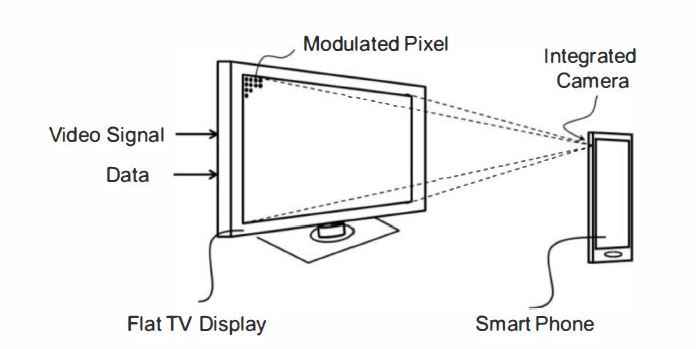
\includegraphics[keepaspectratio,width=0.8\textwidth]{images/David1.jpg}
 \caption{Eine beispielhafte Implementierung des DaViD-Systems}
 \label{fig:David1}
\end{figure}


\section{Systemmodell} 
Bild in Display enthalten eine große Anzahl von Pixeln, die jeweils aus einer spezifischen Anordnung von Subpixeln für die RGB-Farbraum bestehen. Jeder einzelne Frame des Videos wird nämlich durch eine Matrix von Subpixelwerten dargestellt. DaVid System verwendet eine differentielle Modulationsmethod d.h. Teil der Videoinformationen muss wiederholt werden, indem Daten als ein symmetrischer Manchester-Code moduliert und zu den Videosignalkomponenten hinzugefügt werden. In Empfängerseite durch eine zeitliche Synchronisation können die zeitliche \gls{ISI} vermieden werden. Dann nach Verwendung einer örtlichen Synchronisation enthalten einen Differenzbild. Weil die Randbereich des Differenzbilds ungültig ist, verlässt sich die Modulationsgebiet durch die Verfahren in diese Arbeit entdecken. Danach werden die überlagerten Datensequenz durch eine Reihe von Behandlungen vom Videoinhalt getrennt. Abbildung 2.2 zeigt die schematische Darstellung des DaVid-Systems. 
% Deshalb in zeitlicher oder örtlicher Richtung die Videoinhalt in paar Bildern werden gleich.
\vspace{18pt}

\begin{figure}[htb]
	\centering 
	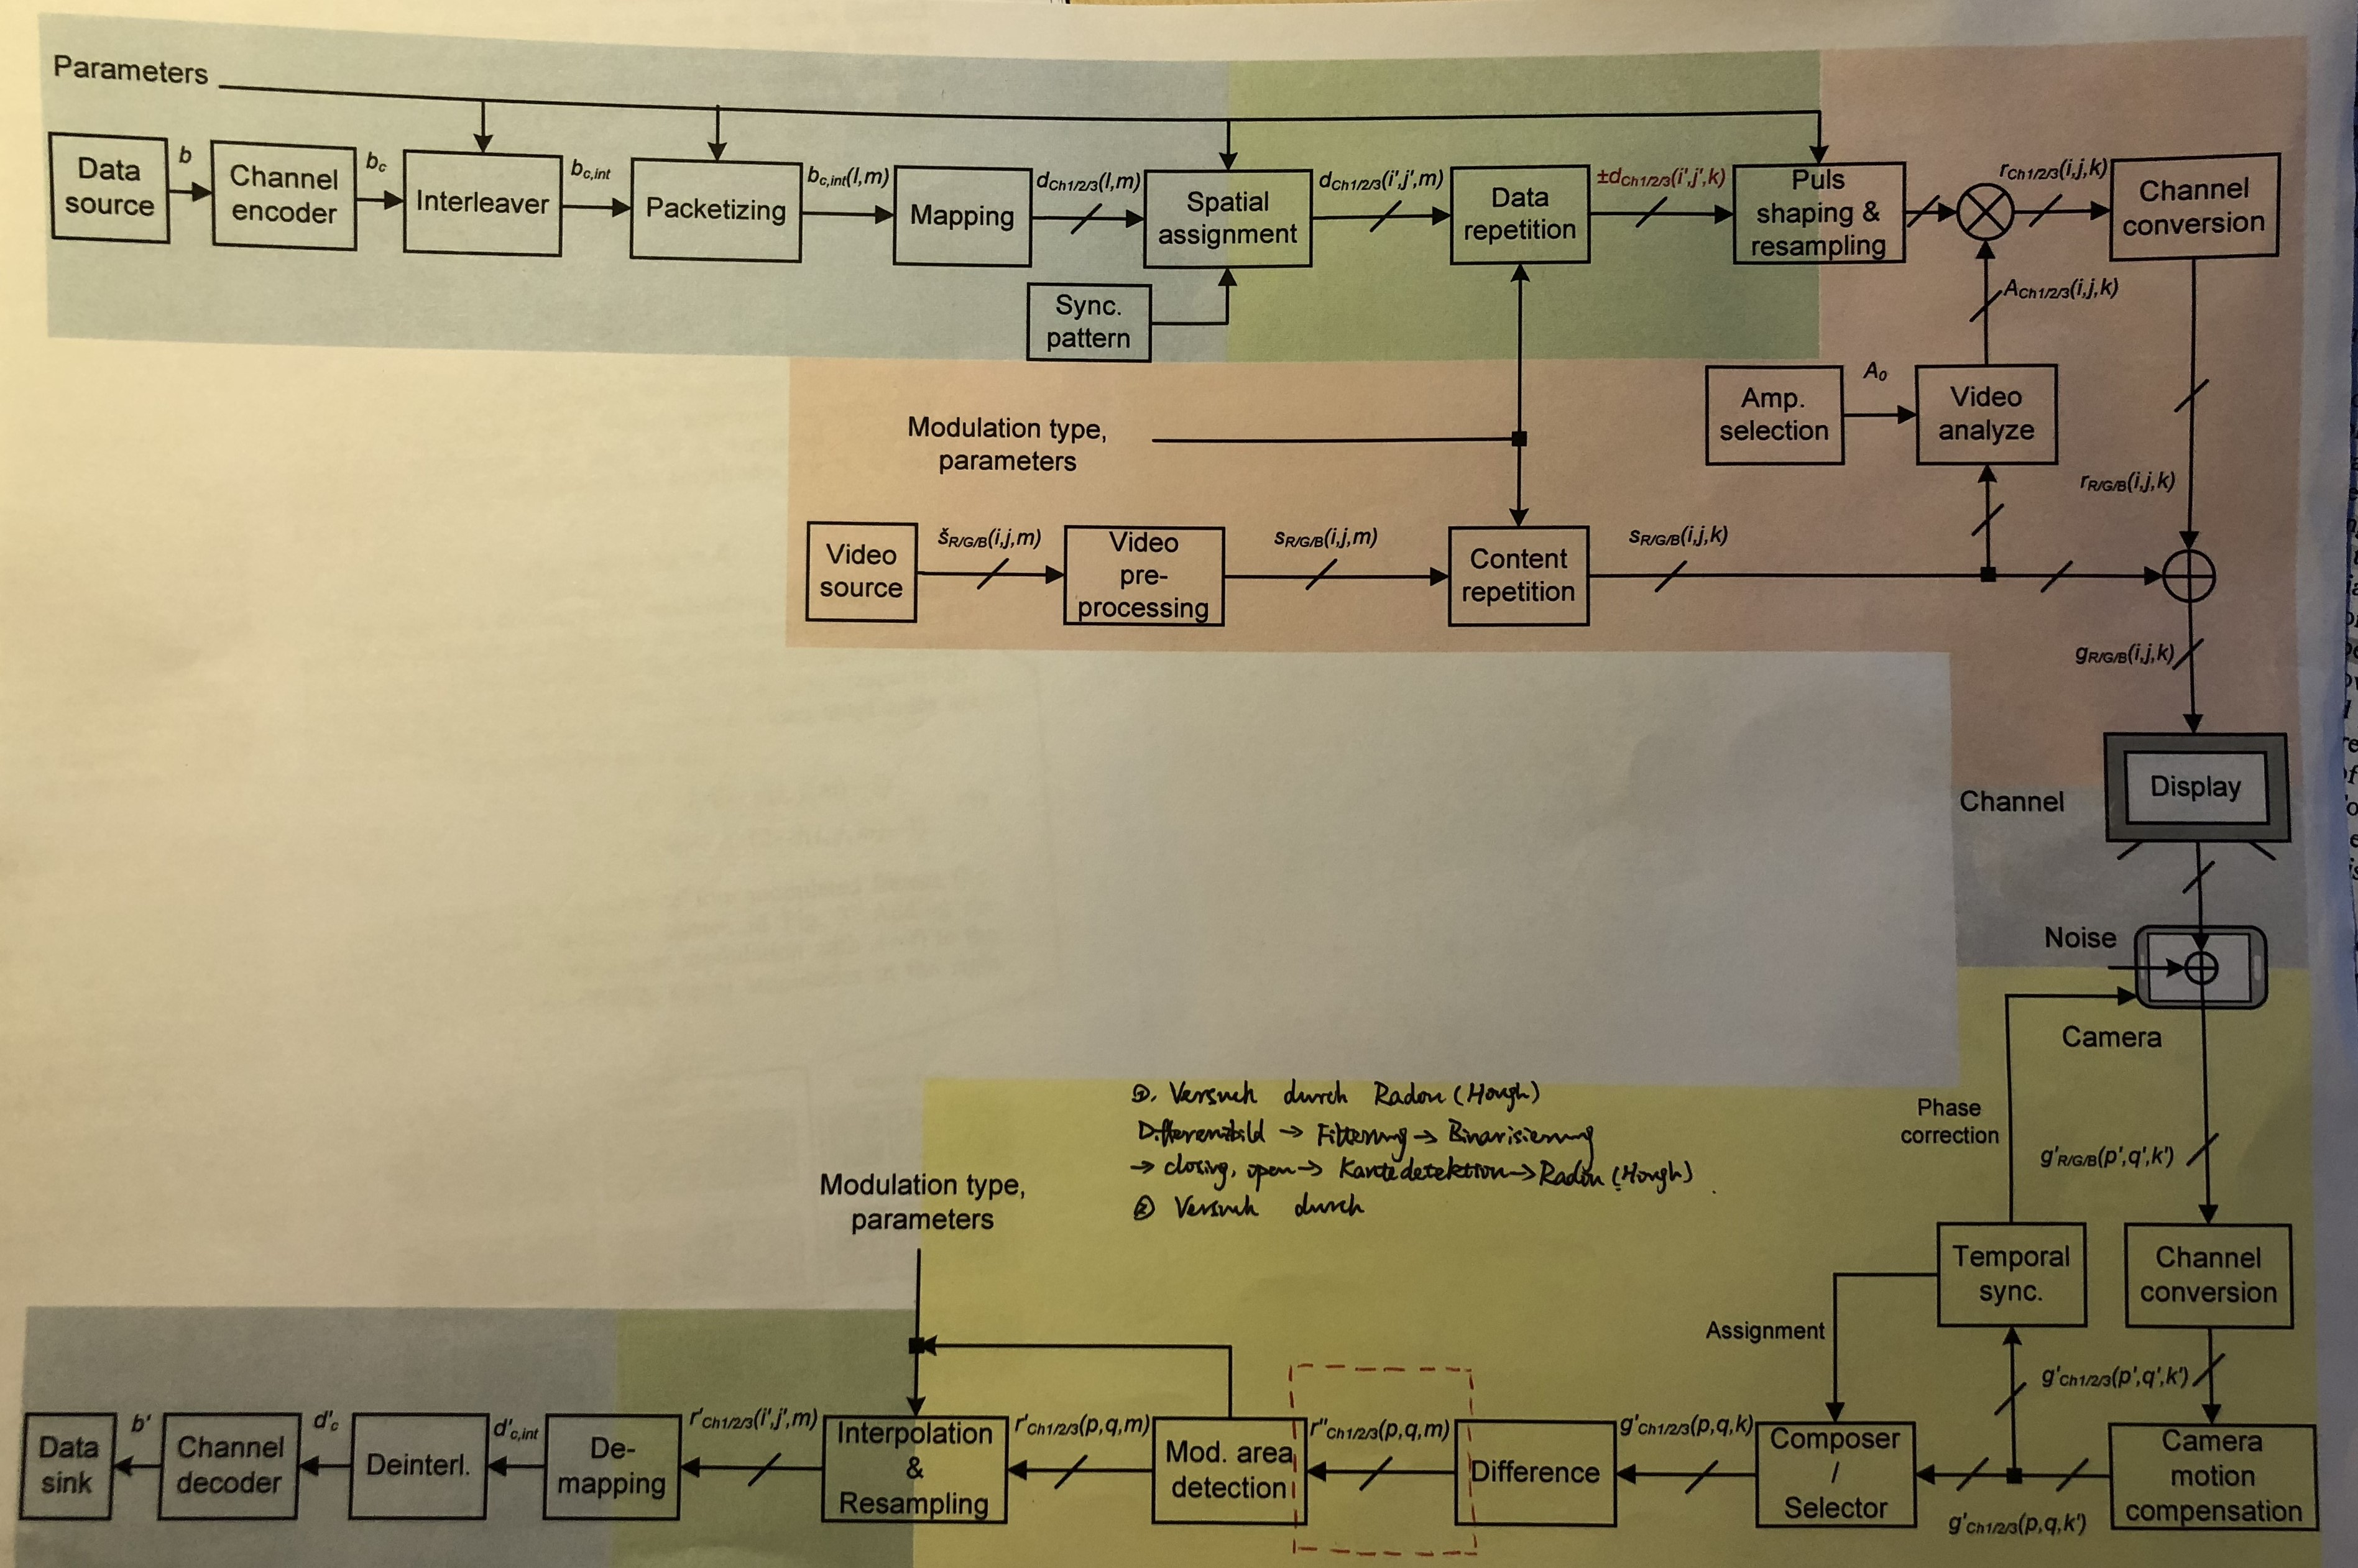
\includegraphics[keepaspectratio,width=1.0\textwidth]{images/David3.jpg}
	\caption{Schematische Darstellung von DaVid System}
	\label{fig:David2}
\end{figure}


\subsection{Modulationsverfahren}

Ein Modulationsverfahren, das die Videoqualität nicht offensichtlich reduziert garantiert, ist sehr wichtig für ein auf Videogerät basierendes Datenübertragungssystem. Die möglichen Modulationsverfahren in DaVid-System sind:
\begin{itemize}
	\item Zeitliche differentielle Modulation der Luminanz
	\item Zeitliche differentielle Modulation der Chrominanz
	\item Örtliche differentielle Modulation der Luminanz
	\item Örtliche differentielle Modulation der Chrominanz
\end{itemize}

Zeitliche differentielle Modulationsverfahre lässt kontinuierliches Paar Frames den gleichen Luminanz- bzw. Chrominanz-Videoinhalt enthalten, d.h. durch Subtrahieren die mit daten addiert Kanal der Paar Frames die Differenzbild erhalten lassen können. Dagegen in örtliche- sind die benachbarte Pixel mit den gleichen Videoamplituden. Im Vergleich zu Luminanzteil Y die Anzeigequalität in U und V Komponente ist signifikant besser, wenn Informationen in Chrominanz wiederholt und moduliert werden. Deswegen wird in dieser Arbeit nur zeitliche differentielle Modulation der Chrominanz verwendet. Abbildung 2.3 zeigt ein Blockdiagramm einer typischen Senderimplementierung durch zeitliche differentielle Modulation.

\begin{figure}[htb]
	\centering 
	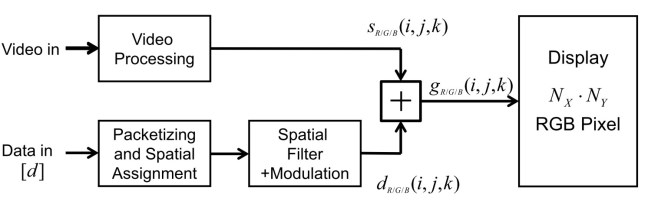
\includegraphics[keepaspectratio,width=0.8\textwidth]{images/David2.jpg}
	\caption{Blockschaltbild der Signalverarbeitung in zeitlicher differentieller Modulation}
	\label{fig:David3}
\end{figure}

Wir nehmen eine Diaplay an, die in horizontale Richtung $N_x$ Pixel stehen, dagegen in vertikale Richtung $N_y$ Pixel. Das Videoeingangssignal wird verarbeitet, um eine Anzeigeeingabe $s(i,j,k)$ zu liefern. Mit zeitliche differenziell Modulation ist die Videoinhalt des kommenden Frame dasselbe.Die Indizes i und j bedeuten die horizontale und vertikale Pixelposition auf dem Bildschirm, während k die Nummer des reproduzierten Bildes ist.
Indiz m heißt den Zähler des Frames in einer Videosequenz. Der Amplitudenbereich des Videosignals sollte begrenzt sein, um die Addition kleiner Datenamplituden ohne Übersteuern zu ermöglichen.

\begin{equation}
\begin{split}
 s_{R/G/B}&(i,j,k+1) = s(i,j,k) \\
          &  for \ 0\le i <N_x, 0\le j<N_y,k=2 \cdot m , m \in \mathbb{Z}\\
\end{split}
\end{equation}

Vor Datenübertragung muss der Datenstrom in Schichten der Länge L aufgeteilt werden. Indiz L bedeutet die Menge der Daten, die in einem Framepaar übertragen werden können. Ein direkter Ansatz ist eine direkte Zuordnung von Datenbits zu Pixeltripeln Zeile für Zeile.

\begin{equation}
\begin{split}
  & d(l)\rightarrow d(i,j,m) \qquad d(l)\in \{-1,1\} \\
  & 0\le l <L,L = N_x \cdot N_y \\
  & i=l \bmod N_x \qquad j=\lfloor l/N_x \rfloor \\
\end{split}
\end{equation}

Die Modulationsamplitude A ist ein wichtiger Parameter für Datenübertragung. Im Prinzip kann die Amplitude in verschieden Kanal unabhängig gewählt werden, um die Systemleistung zu optimieren. In diesen Arbeiten setzen die Amplitude gleichwertig.

\begin{equation}
 A_R=A_G=A_B=A        
\end{equation}

Das differentielle Modulationsverfahren ordnet jede Sequenz von $\left\{-A, A\right\}$ zu d = -1 bzw. $\left\{A, -A\right\}$ zu d = 1 zu. Modulierte Datensymbole und verarbeitete Videoamplituden werden addiert, um die Anzeigeeingabe $g(i,j,k)$ zu liefern:

\begin{equation}
\begin{split}
   s_{R/G/B}(i,j,k)  &= s_{R/G/B}(i,j,m) + A_{R/G/B} \cdot \left( 2 \cdot d(i,j,m) - 1 \right) \\
   s_{R/G/B}(i,j,k+1)&= s_{R/G/B}(i,j,m) - A_{R/G/B} \cdot \left( 2 \cdot d(i,j,m) - 1 \right) \\
\end{split}
\end{equation}

Ein Beispiel einer modulierten Bildfolge ist in Abbildung 2.4 gezeigt. Das Hinzufügen der modulierten Daten (hier mit A = 4) zu dem Videoeingang ergibt die Anzeigeamplituden in der rechten Spalte.
\newpage

\begin{figure}[htb]
	\centering 
	\includegraphics[keepaspectratio,width=0.8\textwidth]{images/David4.jpg}
	\caption{Ein Beispiel einer modulierten Bildfolge}
	\label{fig:David4}
\end{figure}


\begin{equation}
   T = \begin{pmatrix}
   0,213 & 0,715 & 0,072 \\
   -0,115& -0,385& 0,5	\\
   0,5   & -0,454& -0,0458
\end{pmatrix}  
\end{equation}


\begin{equation}
\begin{split}
  \begin{pmatrix}
  g_R(i,j,k) \\
  g_G(i,j,k) \\
  g_B(i,j,k) \\
\end{pmatrix} &= T^{-1} \cdot \left( T \cdot \begin{pmatrix}
  S_R(i,j,m) \\
  S_G(i,j,m) \\
  S_B(i,j,m) 
  \end{pmatrix}  + \begin{pmatrix}
  0 \\
  A_U \cdot d(i,j,m) \\
  A_V \cdot d(i,j,m) 
  \end{pmatrix} \right) \\  
  \begin{pmatrix}
  g_R(i,j,k+1) \\
  g_G(i,j,k+1) \\
  g_B(i,j,k+1) \\
\end{pmatrix} &= T^{-1} \cdot \left( T \cdot \begin{pmatrix}
  S_R(i,j,m) \\
  S_G(i,j,m) \\
  S_B(i,j,m) 
  \end{pmatrix}  - \begin{pmatrix}
  0 \\
  A_U \cdot d(i,j,m) \\
  A_V \cdot d(i,j,m) 
  \end{pmatrix} \right) \\ 
\end{split}
\end{equation}


\begin{equation}
   \begin{pmatrix}
   A_R \\
   A_G \\
   A_B
  \end{pmatrix}  = T^{-1} \cdot \begin{pmatrix}
   A_Y \\
   A_U \\
   A_V
  \end{pmatrix}
\end{equation}



\subsection{DatenBlock}

Um die Anforderungen an die Kameraauflösung zu lockern, Ein einfaches und unkompliziertes Verfahren ist Zuordnung jedes Datenbits zu einem Block von $B_X \times B_Y$ Pixeln.

\begin{equation}
\begin{split}
  & d(l)\rightarrow d(x,y,k) \qquad 0\le l <L \\
  & L=\lfloor N_X/B_X \rfloor \cdot \lfloor N_Y/B_Y \rfloor \\
  & x=(l \cdot B_X) \bmod N_X +r_X, \ r_X =0...(B_X -1) \\
  & y=\lfloor l / \lfloor N_X/B_X \rfloor \rfloor \cdot B_Y +r_Y, \ r_Y =0...(B_Y -1) \\
\end{split}
\end{equation}

Wenn die Anzahl der Pixel pro Zeile kein Vielfaches von $B_X$ ist oder wenn die Anzahl der Pixel kein Vielfaches von $B_Y$ ist, muss die Anzahl der Pixel und Zeilen, die für die Modulation in Gleichung $\left(2.5\right)$ verwendet werden, ersetzt werden durch:

\begin{equation}
\begin{split}
  & N_X = \lfloor N_X/B_X \rfloor \cdot B_X\\ 
  & N_Y = \lfloor N_Y/B_Y \rfloor \cdot B_Y\\ 
\end{split}
\end{equation}

% \newpage
In dieser Arbeit werden das DatenBlock für quadratische Blöcke gesetzt.

\begin{equation}
   B_X = B_Y = B.
\end{equation}





\section{Anwendungsgebiete} 
%\label{sec:Anwendungsbereiche}

Die Datenübertragungsrate des David-Systems wird voraussichtlich erreicht bis zu 100 Mbit/s. Es gehöre	zu einer Sichtlinienübertragung für kurze Verbindungen. Geeignete Abdeckungsbereichen hängen von der Größe des Displays und der Kameraoptik ab. Obwohl im Vergleich zum letzten WLAN- Versionen \gls{ieee} 802.11, die Leistung scheint nicht so attraktiv. Der Vorteil liegt nicht nur in der wachsenden Leistungsfähigkeit von Video-Display und Kamera, aber auch die Option zur Wiederverwendung der bestehenden Hardware, die zum Zeigen des Videos installiert wurde. Ein empfohlene praktische Anwendungsbereich des DaVids ist öffentlicher Ort, z.B. U-Bahn-Station, großes Stadion und so weiter. Annehmen eine Situation, wenn die Leute auf ihre U-Bahn warten, sie können ihre eigene Software aktualisieren, indem Sie einfach auf die zeigende Werbung in dem Bildschirm leiten.

Berücksichtigen der Eigenschaften des DaVids, d.h. die Synchronisation von Videospielen und Datenübertragung. Viele Anwendungsszenarien können in Betracht gezogen werden und scheinen sehr attraktiv zu sein. Die drei Hauptszenarien sind:

\begin{itemize}
  \item Indoor-individuelle Kommunikation: Kurzstreckenverbindungen basieren auf relativ kleinen (Tablet-Größe) Bildschirm, Anwendungen z.B. die Übertragung von Hintergrundinformationen an Besucher im Museum, Kiosk.
  \item Indoor-Multicast-Kommunikation:Streckabstand ist länger als ersten Fall auf relativ größer (40-100") Bildschirm, Anwendungen z.B. während Videoabspielen Besucher die Anwendungsdaten oder Mediendateien herunterladen können im Kiosk, Restaurant.
  \item Freien Kommunikation: Größter Bildschirm wie im Einkaufszentren oder Sport-Arenen, Anwendungen können denen des zweiten Szenarios ähneln.
\end{itemize}

Sobald die Dienste auf öffentlichen Bildschirmen implementiert werden, kann Leute mit Hilfe eines modernen Smartphones, die mit einer geeigneten Kamera eingebaut ist, nach der Installation einer neuen App innovative wahrnehmen.






















\chapter{ErsteErfahrung} \label{cha:ErsteErfahrung}

In diesem Kapitel werden die erste Erfahrung beschrieben. Zuerst läuft die Vorstellung des DaVid-Systems. Die Systemmodell und Arbeitsprinzip des Systems werden in anschließenden Abschnitt erläutert. Schließlich folgt die mögliche Anwendungsgebiete des Systems.

Nicht vergessen, dass Überschriften nicht aufeinander folgen dürfen\ldots

\begin{otherlanguage}{english}
\section{TexLipse spell checking}
%
To enable spell checking in TeXLipse, download the respective dictionaries from 
\url{https://sourceforge.net/projects/texlipse/files/dictionaries/}.

Save the dictionaries at a local location and enter the path in \texttt{Window->Preferences->Tex\-lipse->Spell Checker} (see Fig. \ref{fig:dict_path}).
%
\begin{figure}[htb]
	\centering
	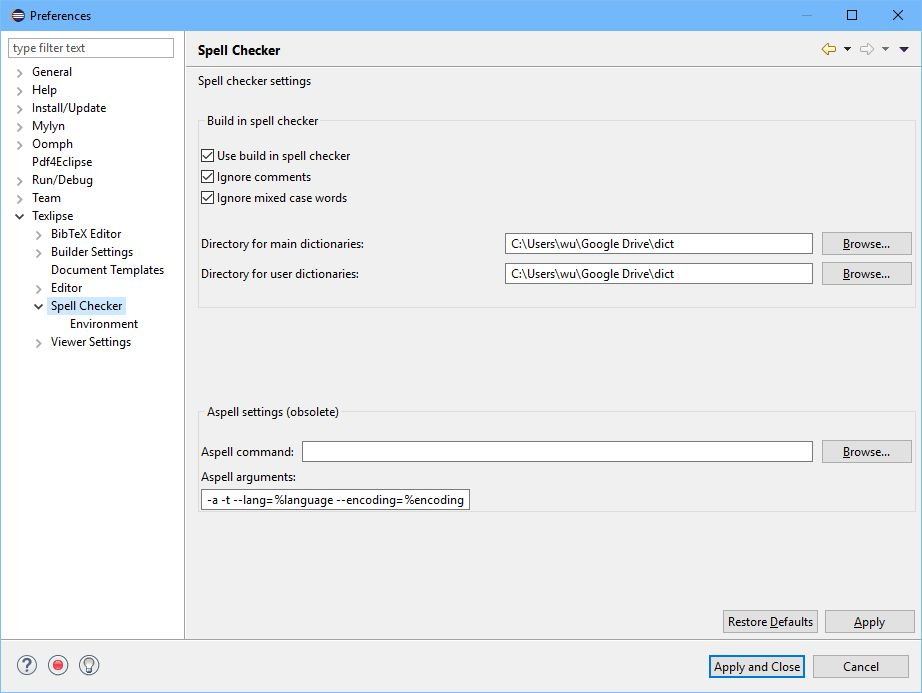
\includegraphics[scale=0.40]{images/Spell_Checker_preferences.jpg}
	\captionbelow{TeXLipse Spell Checker preferences}
	\label{fig:dict_path}
\end{figure}

To synchronize the user dictionaries between multiple machines, it might be useful to save the dictionaries in your google drive or drop box.

\section{Enable tikzexternalize for PdfLatex}

Go to \texttt{Window->Preferences->Texlipse->Builder Settings} and add 
%
\begin{verbatim}
--shell-escape
\end{verbatim}
%
to the command arguments (see Fig. \ref{fig:builder_settings}).
%
\begin{figure}[htb]
	\centering
	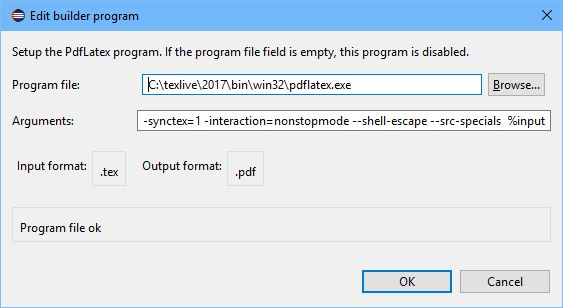
\includegraphics[scale=0.40]{images/PdfLatex_settings.jpg}
	\captionbelow{PdfLatex Builder Settings}
	\label{fig:builder_settings}
\end{figure}

\section{Forward search with TeXlipse and Sumatra PDF}

Download and install SumatraPDF: \url{https://www.sumatrapdfreader.org/}.

Then edit the viewer settings for SumatraPDF in \texttt{Window->Preferences->Texlipse->Viewer Settings}.

Change the viewer arguments to
%
\begin{verbatim}
-reuse-instance %fullfile -forward-search %texfile %line
\end{verbatim}
%
and leave all DDE message field empty.
Change the inverse search support to "`Viewer runs external command"' and enable "`Viewer supports forward search"'.

Figure \ref{fig:viewer_settings} displays the dialog window.
%
\begin{figure}[htb]
	\centering
	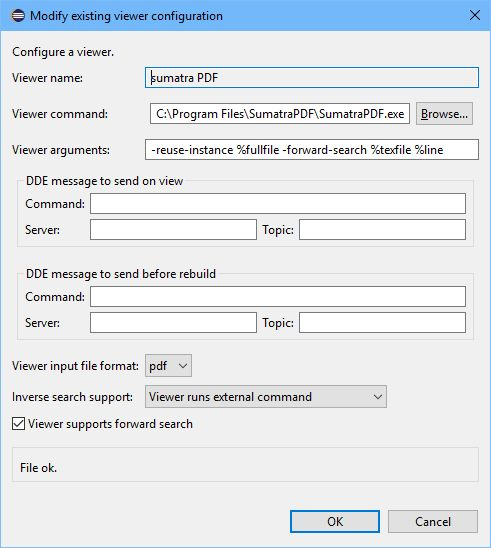
\includegraphics[scale=0.40]{images/Viewer_settings.jpg}
	\captionbelow{TeXLipse Viewer Settings}
	\label{fig:viewer_settings}
\end{figure}

In SumatraPDF configure the inverse search command via the \texttt{Settings->Options} menu (see Fig. \ref{fig:sumatrapdf_options}).
%
\begin{figure}[htb]
	\centering
	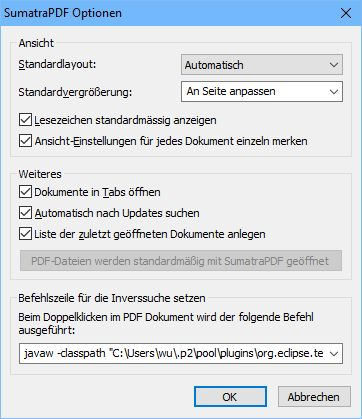
\includegraphics[scale=0.40]{images/SumatraPDF_optionen.jpg}
	\captionbelow{SumatraPDF Options}
	\label{fig:sumatrapdf_options}
\end{figure}

If you have install TeXlipse~1.5.0, the inverse search command will look like this:

\begin{lstlisting}[breaklines=true, basicstyle=\ttfamily, columns=flexible]
javaw -classpath "C:\Users\wu\.p2\pool\plugins\net.sourceforge.texlipse_1.5.0\texlipse.jar" net.sourceforge.texlipse.viewer.util.FileLocationClient -p 55000 -f "%f" -l %l
\end{lstlisting}

Let the path point to your eclipse share pool. Or if you do not have a shared pool, choose the plugins directory of your eclipse installation.

For TeXLipse~2.0.X the FileLocationClient is relocated to org.eclipse.texlipse making the inverse search command look like the following.
\begin{lstlisting}[breaklines=true, basicstyle=\ttfamily, columns=flexible]
javaw -classpath "C:\Users\wu\.p2\pool\plugins\org.eclipse.texlipse_2.0.1.201801202105\texlipse.jar" org.eclipse.texlipse.viewer.util.FileLocationClient -p 55000 -f "%f" -l %l
\end{lstlisting}

\end{otherlanguage}
\chapter{Zweite Methode} \label{cha:Zweite Methode}

In diesem Kapitel wird die Realisierung des zweiten Verfahrens eingegangen werden. Die Bildregistrierung wird zuerst im Detail gegeben. Anschließen läuft die Differenzbild Optimierung und Bildverarbeitung. QR Muster Detektion und die entspricht Matlab Code werden schließlich erläutert. 
Zur Implementierung dieser Verfahre wird Matlab unter der Lizenz TU Dortmund verwendet.

\section{Allgemeine Struktur} 

Dieses Verfahren verwendet die Charakteristiken der Datenmodulation des DaViD Systems, d.h. an jedem Eck des Datenebene ein QR Muster hinzu und dann mit den Daten zusammen hinter dem Bild moduliert. Am Empfängen  durch eine Reihe von Verarbeitungen wird QR Muster detektiert wird und dann schließlich bestimmt der Modulationsbereich. Diese Methode löst effektiv den unschönen Effekt, der das QR-Modul direkt zum Bild hinzugefügt wird, und kann das Problem schnell und effektiv durch die QR-Mustereigenschaft lösen. Abbildung 4.1 zeigt die Strukturdiagramm des Verfahrens.

In dieser Verfahre läuft zuerst Bildregistrierung. Durch diese Schritt kann die Punkte über den zwei Bildern in dasselbe Koordinatensystem konvertieren. Anschließen mit Helfe einen Optimierung für die enthaltet Differenzbilder wird eine detektierend Bild bekommen, die die Erkennung des QR Musters erleichtern können. Schließlich wird es durch die Charakteristik des QR Musters, das Breiteverhältnis $1:1:3:1:1$ beträgt, um QR Muster zu detektieren.

\begin{figure}[H]
 \centering 
 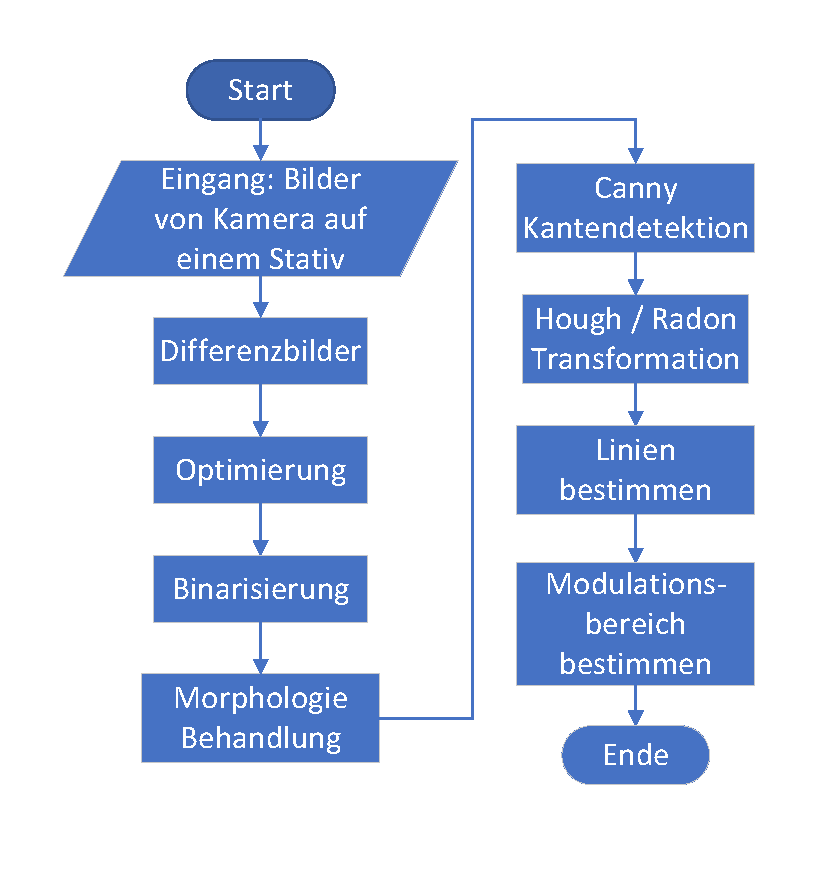
\includegraphics[keepaspectratio,width=1.0\textwidth]{images/4_ZweiteErfahrung/Flussdiagrammsum.pdf}
 \caption{Flussdiagramm der Methode}
 \label{fig:Flussdiagramm der Methode}
\end{figure}

\section{Bildregistrierung} 

Annehmen eine Szene, wenn eine Rhein Fotos mit einer Handheld-Kamera aufnehmen, kommt es aufgrund von Handbewegungen zu einer leichten Verschiebung zwischen den beiden benachbarten Fotos. Wenn Sie diese Fotos abziehen, um Differenzbild zu erhalten, wird der Ergebnisse sehr schlecht sein. Um diese Problem zu lösen, wird hier Bildregistrierung eingeführt. Ein Flussdiagramm der Bildregistrierung wird in Abbildung 4.2 gezeigt. 

\begin{figure}[H]
 \centering 
 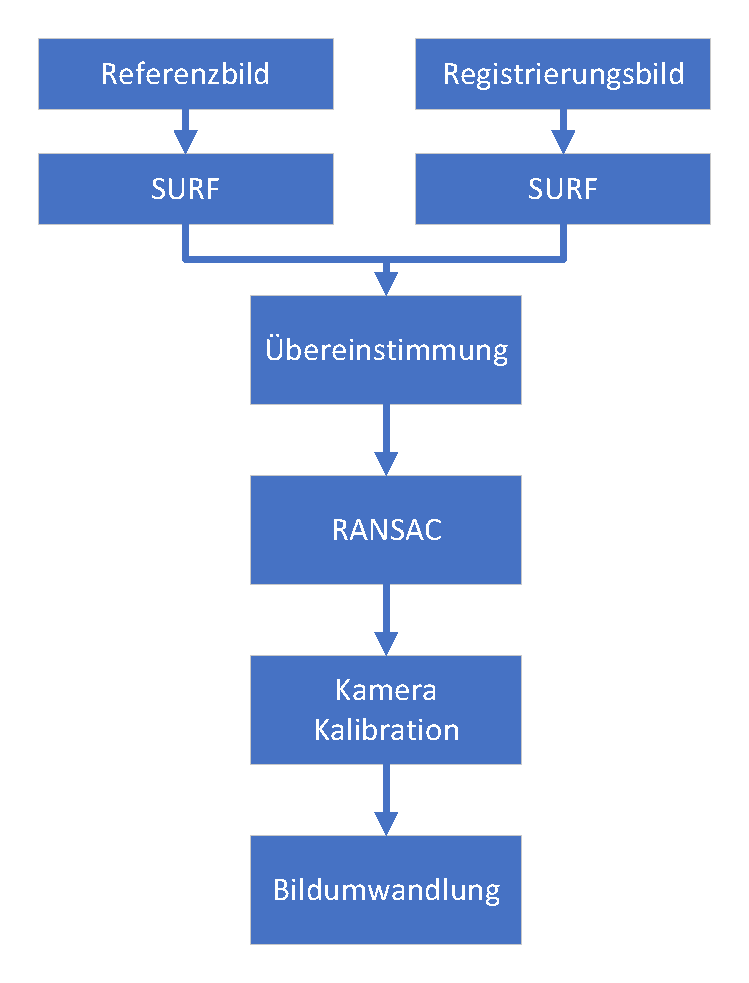
\includegraphics[keepaspectratio,width=0.6\textwidth]{images/4_ZweiteErfahrung/Bildregistration.pdf}
 \caption{Flussdiagramm der Bildregistrierung}
 \label{fig:Bildregistrierung}
\end{figure}

\subsection{SURF}
In Bildregistrierung wird zuerste Merkmalserkennung eingegangen. Hier in dieser Arbeite lass die SURF \cite{Surf} nutzen. Es ist eine verbesserte Version von SIFT, die Haar-Wavelet verwendet, um die Gradientenoperation in der SIFT-Methode anzunähern und gleichzeitig verwendet eine Integralgraph-Technik für schnelle Berechnungen. Die Faltung bezieht sich nur auf das vorherige Bild, mit Erhöhung der Größe des Bildkerns können das Heruntertaktung-Verfahren realisiert werden. Die Geschwindigkeit von SURF ist 3-7 mal die von SIFT mit der in den meisten Fällen entspricht   Leistung von SIFT. Daher wurde es in vielen Anwendungen eingesetzt, insbesondere in Anwendungen, in denen die Laufzeitanforderungen hoch sind. Der Verläuf einer SURF Merkmalserkennung ist wie flogend:

$\bullet$ \textbf{Aufbau einer hessischen Matrix.}\\
Die Hesse-Matrix stellt den Kern des SURF Algorithmus dar. Zur Vereinfachung der Operation wird die Funktion f (z, y) angenommen, dass die Hesse-Matrix H setzt sich aus Funktionen und partiellen Ableitungen zusammen:

\begin{equation}
   \mathcal{H}(f(x,y)) = \begin{bmatrix}
   \frac{\partial^{2}f}{\partial x^{2}} & \frac{\partial^{2}f}{\partial x \cdot \partial y} \\
   \frac{\partial^{2}f}{\partial x \cdot \partial y} & \frac{\partial^{2}f}{\partial y^{2}} \\   
   \end{bmatrix}
\end{equation}

 Diskriminante der H-Matrix läuft:
 
\begin{equation}
   \det(\mathcal{H}) = \frac{\partial^{2}f}{\partial x^{2}} \cdot \frac{\partial^{2}f}{\partial y^{2}} - (\frac{\partial^{2}f}{\partial x \cdot \partial y})^2  
\end{equation}

Der Wert der Diskriminante ist der Eigenwert der H-Matrix. Durch dessen positiven und negativen wird bestimmt, ob der Punkt ein Extrempunkt ist oder nicht. Im SURF Algorithmus wird das Bildpixel $l(x,y)$ anstelle des Funktionswertes $f(x,y)$ verwendet. Nutzen eine Zweite-Order Gaussian Function als Filter. Die zweiten Partielle Ableitungen können durch Faltung zwischen bestimmten Kernen berechnet werden. Dadurch können die Werte der drei Matrixelemente der H-Matrix auch berechnet werden, nämlich die H-Matrix berechnet:

\begin{equation}
\begin{split}
   &\mathcal{H}(\textbf{x},\sigma) = \begin{bmatrix}
   L_{xx}(\textbf{x},\sigma)\ L_{xy}(\textbf{x},\sigma) \\
   L_{xy}(\textbf{x},\sigma)\ L_{yy}(\textbf{x},\sigma)
   \end{bmatrix} \\   
   &L(\textbf{x},\sigma) = G(\sigma)*I(\textbf{x}) \\  
   &G(\sigma) = \frac{\partial^{2}g(\sigma)}{\partial x^{2}}      
\end{split}
\end{equation}


Hier $L_{xx}(\textbf{x},\sigma)$ bedeutet die Faltung der zweiter Gaussian Ableitung $G(\sigma)$ mit dem Bild I in Punkt $\textbf{x}$(x,y), ähnlich für $L_{xy}(\textbf{x},\sigma)$ und $L_{yy}(\textbf{x},\sigma)$. Auf diese Weise kann der Wert der Determinante für jedes Pixel in dem Bild berechnet werden, und dieser Wert kann verwendet werden, um den Merkmalspunkt zu feststellen.
Zur einfacheren Anwendung schlägt Herbert Bay\cite{Surf} vor, L mit einer Approximation ersetzen. Um den Fehler zwischen dem genauen Wert und der Approximation auszugleichen, kann die H-Matrix-Diskriminante wie folgt ausgedrückt werden:

\begin{equation}
   \det(\mathcal{H}_{Approx}) = D_{xx}D_{yy} - (0.9D_{xy})^2  
\end{equation}
\\
$\bullet$ \textbf{Erstellen Maßstab Raum}\\
Der Maßstabsraum $L(\textbf{x},\sigma)$ des Bildes ist die Darstellung dieses Bildes bei unterschiedlichen Auflösungen(Skalierung). Im Bereich der Computer Vision wird der Maßstabsraum symbolisch als Bildpyramide ausgedrückt, wobei die Eingangsbildfunktion wiederholt mit dem Kern der Gaußschen Funktion gefaltet und wiederholt unterabgetastet wird. Diese Methode wird hauptsächlich für die Implementierung des SIFT Algorithmus verwendet. Jede Bildschicht hängt jedoch von der vorherigen Bildschicht ab, und das Bild muss in der Größe angepasst werden. Daher hat diese Berechnungsmethode eine große Kosten in Berechnung. Im Vergleich dazu ist es in SURF durch die Erhöhung der Größe des Bildkerns. Diese ist ein Unterschied zwischen dem SIFT Algorithmus und dem SURF Algorithmus bei der Verwendung des Pyramidenprinzips.
Der Algorithmus ermöglicht, dass mehrere Bilder des Maßstabsraums gleichzeitig verarbeitet werden, ohne dass das Bild unterabgetastet wird, wodurch die Leistung des Algorithmus verbessert wird. Das linke Bild in Abbildung 4.3 ist eine Pyramidenstruktur, die auf herkömmliche Weise erstellt wird, die Größe des Bildes wird geändert, und die Operation wird die Unterebene  unter Verwendung der Gaußschen Funktion wiederholt glätten. Der Surf Algorithmus auf der rechten Seite in Abbildung 4.3 behält das ursprüngliche Bild unverändert und ändert nur die Filtergröße.

\begin{figure}[htb]
 \centering 
 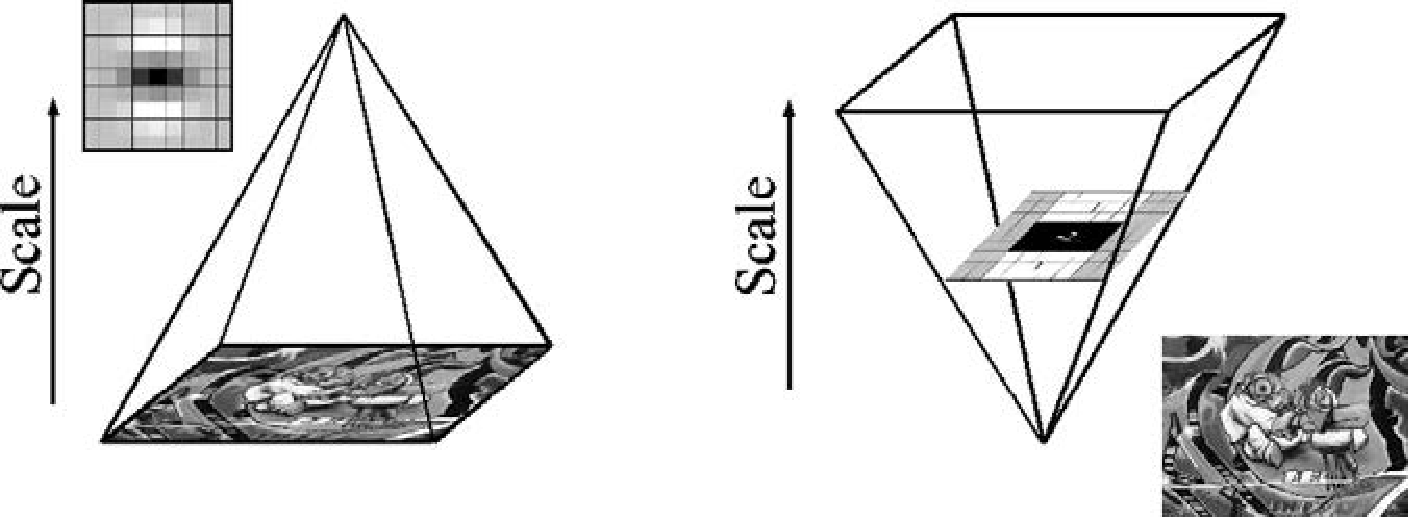
\includegraphics[keepaspectratio,width=0.8\textwidth]{images/4_ZweiteErfahrung/Scale_space.pdf}
 \caption{Scale space}
 \label{fig:Scale space}
\end{figure} 


$\bullet$ \textbf{Präzise Lokalisierung von Feature-Punkten}\\
Vergleichen die Größe jedes Pixel, die von der hessischen Matrix verarbeitet wird, mit die 26 Punkten in seiner drei Dimensionen Raum, wie in Abbildung 4.4 zeight. Wenn es das Maximum oder Minimum dieser 26 Punkte ist, wird es als vorläufiger Merkmalspunkt beibehalten. Das dreidimensionale lineare Interpolationsverfahren wird verwendet, um die Merkmalspunkte des Subpixel-Niveaus zu erhalten, und die Punkte, deren Werte kleiner als ein bestimmter Schwellenwert sind, werden ebenfalls entfernt.

\begin{figure}[htb]
 \centering 
 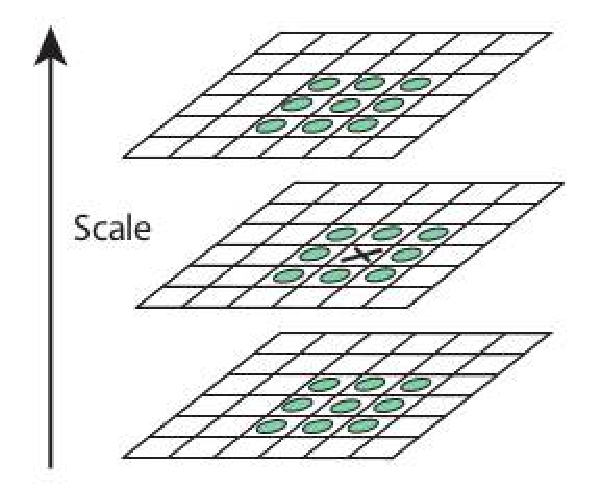
\includegraphics[keepaspectratio,width=0.4\textwidth]{images/4_ZweiteErfahrung/Extreme_Wert_Erkennung.pdf}
 \caption{Extreme Wert Erkennung}
 \label{fig:Extreme Wert Erkennung}
\end{figure} 


$\bullet$ \textbf{Hauptrichtungsermittlung}\\
SIFT wählt die Hauptrichtung des Merkmalspunkts unter Verwendung des Gradientenhistogramms im Merkmalspunktbereich aus. Die Richtung, in der der Bin-Wert des Histogramms der größte und oder 80\% maximale Bin-Wert  überschreitet, wird als Hauptrichtung des Merkmalspunkts genommen. Dagegen beim SURF wird das Gradientenhistogramm nicht statistiken, sondern das Harr-Wavelet-Eigenshcaft im Merkmalspunktbereich wird statistisch analysiert. Das heißt, im Bereich der Merkmalspunkt (zum Beispiel innerhalb eines Kreises mit einem Radius von 6s, wobei s der Maßstab ist, auf dem der Punkt liegt) die Summe der Horizontal-Haar-Wavelet-Merkmale und der Vertikal-Haar-Wavelet-Merkmale aller Punkte im  60-Grad-Sektor($\pi/3$) werden gezählt. Die Größe des Haar Wavelets stellt als 4s, so dass für jeden Sektor einen Wert bekommt. Dann wird 60-Grad-Sektor in einem bestimmten Intervall gedreht, schließlich lassen die Richtung des Sektors mit Maximalwert als Hauptrichtung des Merkmalspunkts nehmen. Ein schematisches Diagramm des Prozesses ist wie folgt in Abbildung 4.5.

\begin{figure}[htb]
 \centering 
 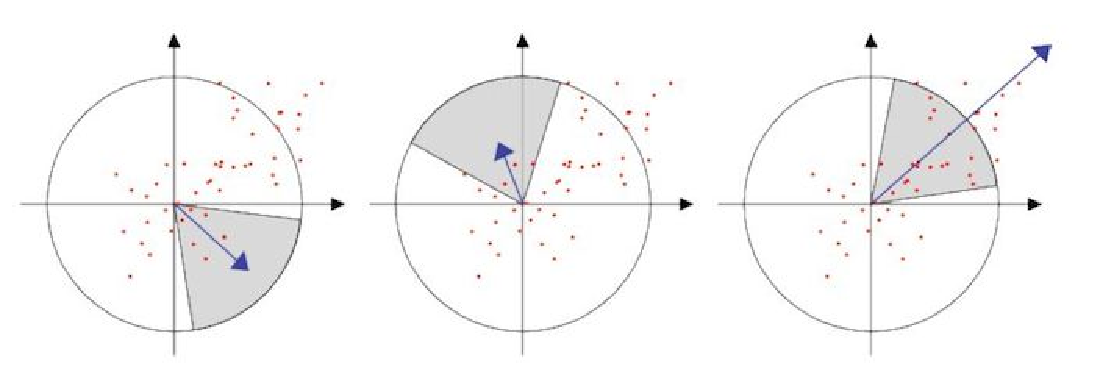
\includegraphics[keepaspectratio,width=0.8\textwidth]{images/4_ZweiteErfahrung/Dominante_Orientierung_Feststellen.pdf}
 \caption{Dominante Orientierung Feststellen}
 \label{fig:Dominante Orientierung Feststellen}
\end{figure} 


$\bullet$ \textbf{Merkmalspunkt Deskriptor Generierung}\\
SURF nehmen eine quadratische Rahmen um den Merkmalspunkt. Die Seite der Rahmen ist 20s (s ist die Skala, bei der der Merkmalspunkt erkannt wird). Die Richtung des Rahmens ist natürlich die Hauptrichtung, die in vorliegened Schritt erfasst wird. Die Rahmen wird dann in 16 Unterbereiche unterteilt, von denen jeder die Haar-Wavelet-Merkmale der horizontalen und vertikalen Richtungen von 25 Pixeln berechnen. Hier die horizontalen und vertikalen Richtungen sind relativ zur Hauptrichtung. Das Haar Wavelet-Merkmal ist die Summe der horizontalen Richtungswerte, die Summe der absoluten Werte in der horizontalen Richtung, die Summe der vertikalen Richtungen und die Summe der absoluten Werte in der vertikalen Richtung. Das schematisches Diagramm in Abbildung 4.6 zeigt dieses Prozesse.

\begin{figure}[htb]
 \centering 
 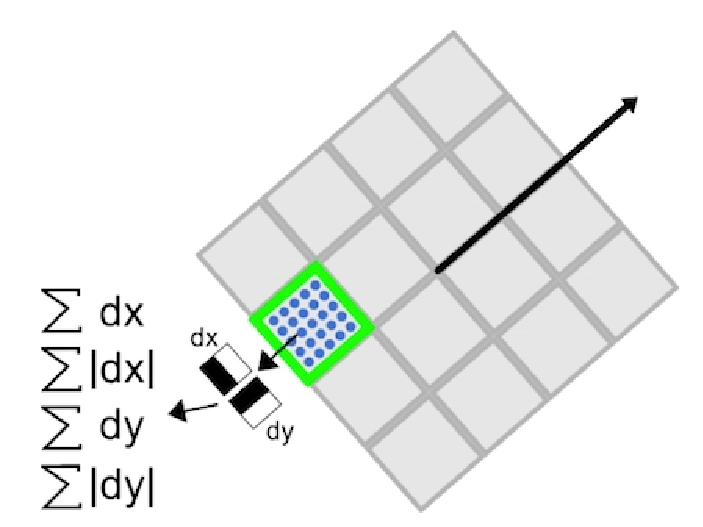
\includegraphics[keepaspectratio,width=0.5\textwidth]{images/4_ZweiteErfahrung/Merkmalspunkt_Deskriptor.pdf}
 \caption{Merkmalspunkt Deskriptor}
 \label{fig:Merkmalspunkt Deskriptor}
\end{figure} 

Auf diese Weise hat jeder kleine Bereich 4 Werte, so dass jeder Merkmalspunkt ein $16*4=64$ dimensionaler Vektor verfügt, der halb so klein wie Sift(128 Dimension) ist, deswegen den Anpassungsprozess beim Merkmalanpassungsprozess stark beschleunigt. Die folgende Abbildung 4.7 zeigt den Merkmalspunkt, den wir durch den SURF-Algorithmus erhalten haben.

\begin{figure}[H]
 \centering 
 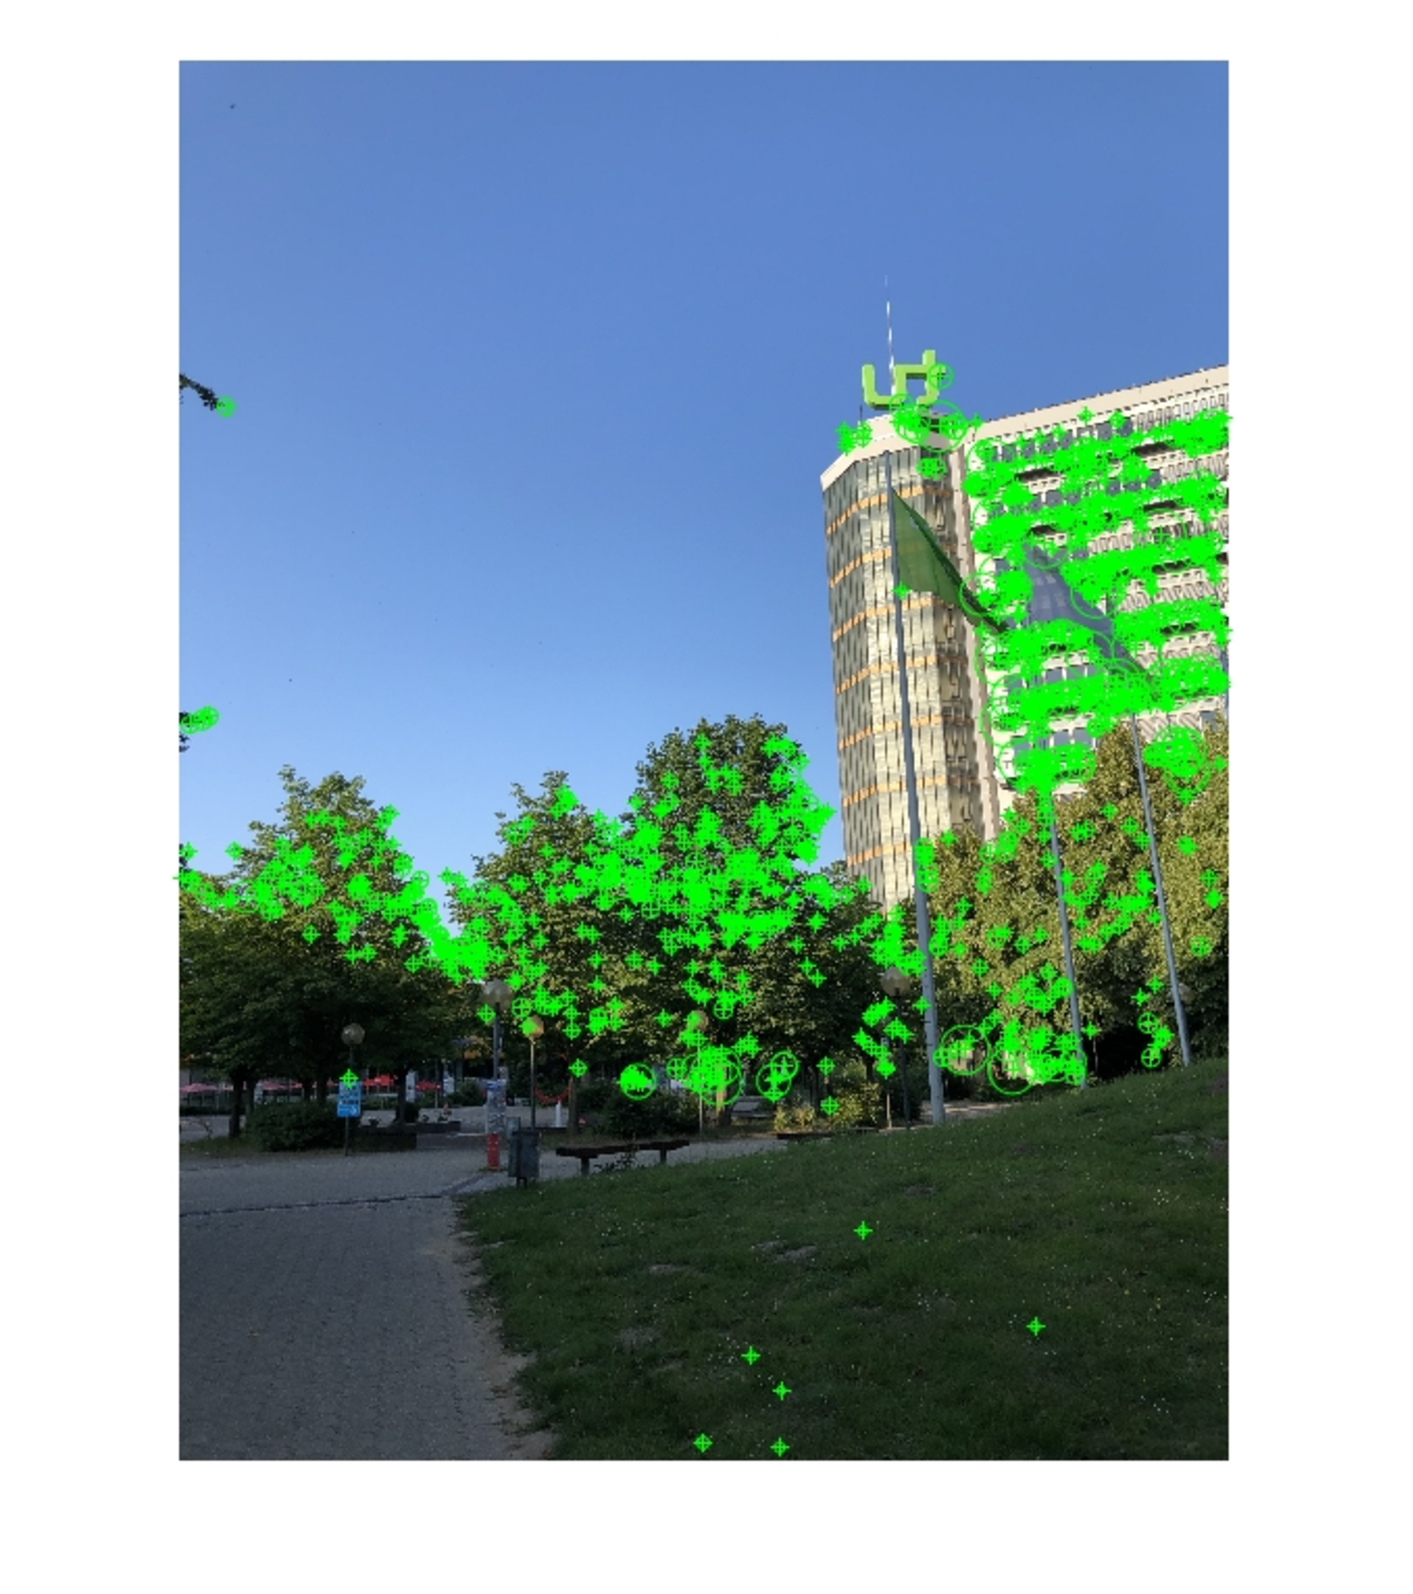
\includegraphics[keepaspectratio,width=0.8\textwidth]{images/4_ZweiteErfahrung/SURF_Detektion.pdf}
 \caption{SURF Merkmal}
 \label{fig:SURF Merkmal}
\end{figure} 


\subsection{RANSAC}

Nach SURF Merkmalserkennung wird die Merkmalspunkte von zwei benachbarten Bildern mit Verfahre z.B. \gls{ncc} übereinstimmt. Leider durch diese Verfahren gibt es noch viele fehlerhafte zusammenpassendes Paar. Deswegen wird \gls{ransac} eingeführt.

RANSAC Algorithmus, der von Fischler und Bolles \cite{ransac1} vorgeschlagene im Jahr 1981, ist ein allgemeiner Parameterschätzungsansatz, um den großen Anteil von Ausreißern in den Eingabedaten zu bewältigen. Im Gegensatz zu vielen der üblichen robusten Schätzverfahren wie M-Schätzer und kleinsten Quadraten, die von der Computer Vision Community aus der Statistik-Literatur übernommen wurden, wurde RANSAC aus der Computer-Vision-Community entwickelt. 

Ein einfaches Beispiel ist in der Abbildung 4.7 dargestellt. Das Ziel besteht darin, die am besten geeignete Linie unter einer Menge von Datenpunkten zu finden. Wenn es die einfache Methode der kleinsten Quadrate verwenden ,um diese Linie zu finden, wie auf der linken Seite gezeigt, kann es leider nicht richtig finden, da die Methode der kleinsten Quadrate von alle Datenpunkte beeinflusst wird. Dagegen mit RANSAC kann das Modell nur von der inlierer Punkte berechnet werden und die Ergebnisse wie auf der rechten Seite zeigt. 

\begin{figure}[H]
 \centering 
 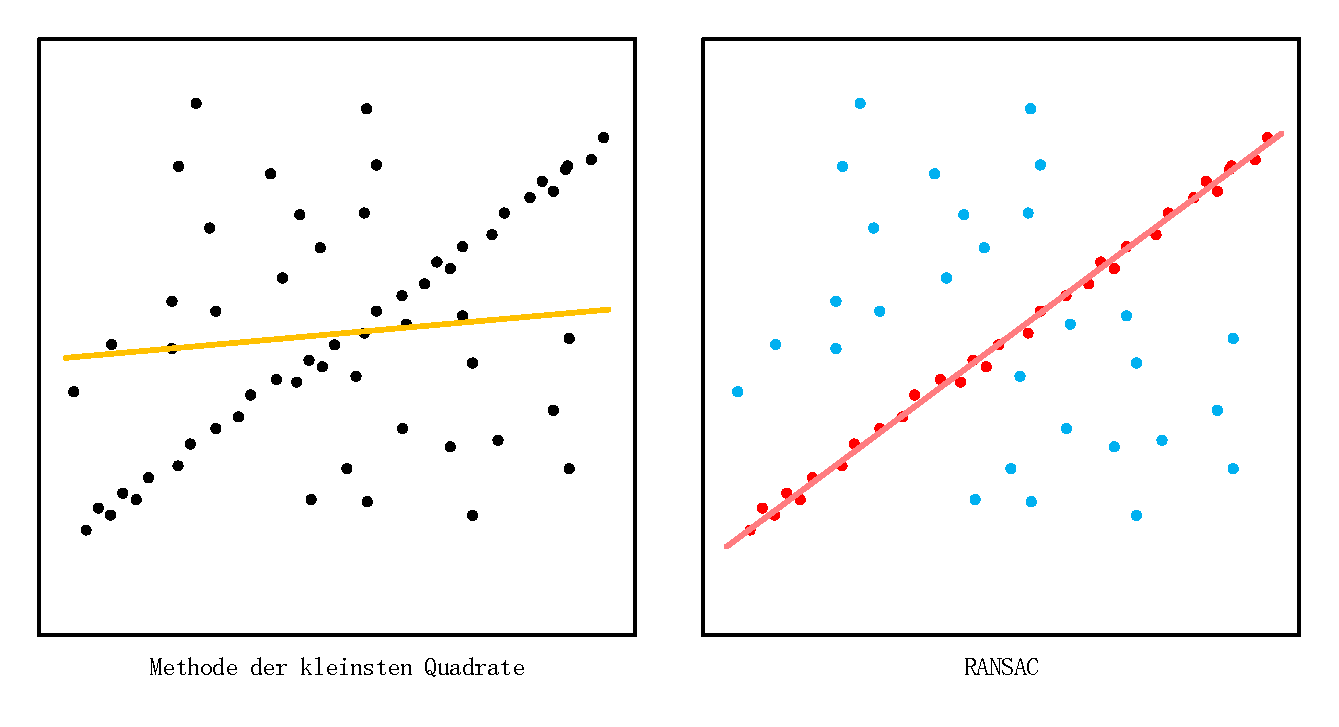
\includegraphics[keepaspectratio,width=1.0\textwidth]{images/4_ZweiteErfahrung/RANSAC/Linien_Detektion.pdf}
 \caption{Linien Detektion}
 \label{fig:Linien Detektion}
\end{figure} 

RANSAC ist ein Wiederholungsprobennahme Verfahren, das  durch die minimalen Anzahl von Beobachtungenpunkten (Datenpunkten) die Kandidatenlösungen generiert. Diese Datebpunkten sind die erforderlich, um die zugrunde liegenden Modellparameter zu schätzen. Darauf haben Fischler und Bolles~\cite{ransac1} hingewiesen, zur Erhalten einer anfängliche Lösung und Beschneidung der Ausreißern RANSAC Verfahren baraucht nicht so viele Daten, sondern verwendet die kleinste mögliche Menge und fährt fort, diese Menge mit eine konsistenten Datenpunkten zu vergrößern.

Der grundlegende Algorithmus ist wie folgt zusammengefasst:

\begin{itemize}
	\item Zufällig wählen die Mindestanzahl der Punkten aus, die erforderlich sind, zum Bestimmen der Modellparameter.
	\item Lösen die Parameter des Modells.
	\item Bestimmen wie viele Punkte aus der Menge aller Punkte mit einer vordefinierten Toleranz $\epsilon$ übereinstimmen
	\item Wenn der Bruchteil der Anzahl von Inlierern über die Gesamtzahl der Punkte in dem Satz einen vordefinierten Schwellenwert $\tau$ überschreitet, schätzen die Modellparameter mit allen identifizierten Inlierern und terminieren wieder.
	\item Ansonsten wiederholen die Schritte 1 bis 4 (maximal N-mal).
\end{itemize}

N bedeutet die Anzahl der Iterationen. Es wird hoch genug gewählt, um die Wahrscheinlichkeit p (normalerweise auf 0,99 gesetzt) sicherzustellen, dass mindestens eine der Gruppen von Stichproben keinen Ausreißer enthält.
Dann die Wahrscheinlichkeit, dass bei N Mal Iterationen mit erforderlich minimalen Anzahl Punkte (hier m annahmen) mindestens ein Ausreißer mit ausgewählt wird, läuft:

\begin{equation}
   1 - p = (1 - u^m)^N
\end{equation}

Hier u stellen die Wahrscheinlichkeit dar, dass jeder ausgewählte Datenpunkt ein Inlier ist. Dagegen $v = 1 - u$ heißt die Wahrscheinlichkeit, dass jeder ausgewählte Datenpunkt ein Ausreißer ist. Durch einige Gleichheitsumwandlung können die Anzahl der Iterationen ausgedrückt werden als:

\begin{equation}
   N = \frac{\log(1 - p)}{\log(1 - (1 - v)^m)}
\end{equation}

Abbildung 4.8 zeigt die passende Punkt durch SURF Merkmalserkennung. Es ist ersichtlich, dass es viele fehlerhafte Kombinationen gibt. Durch die Anwendung von RANSAC kann dieses Problem effektiv lösen und die übereinstimmendenPunkte verfeinern, wie in Abbildung 4.9 zeigt.

\begin{figure}[H]
 \centering 
 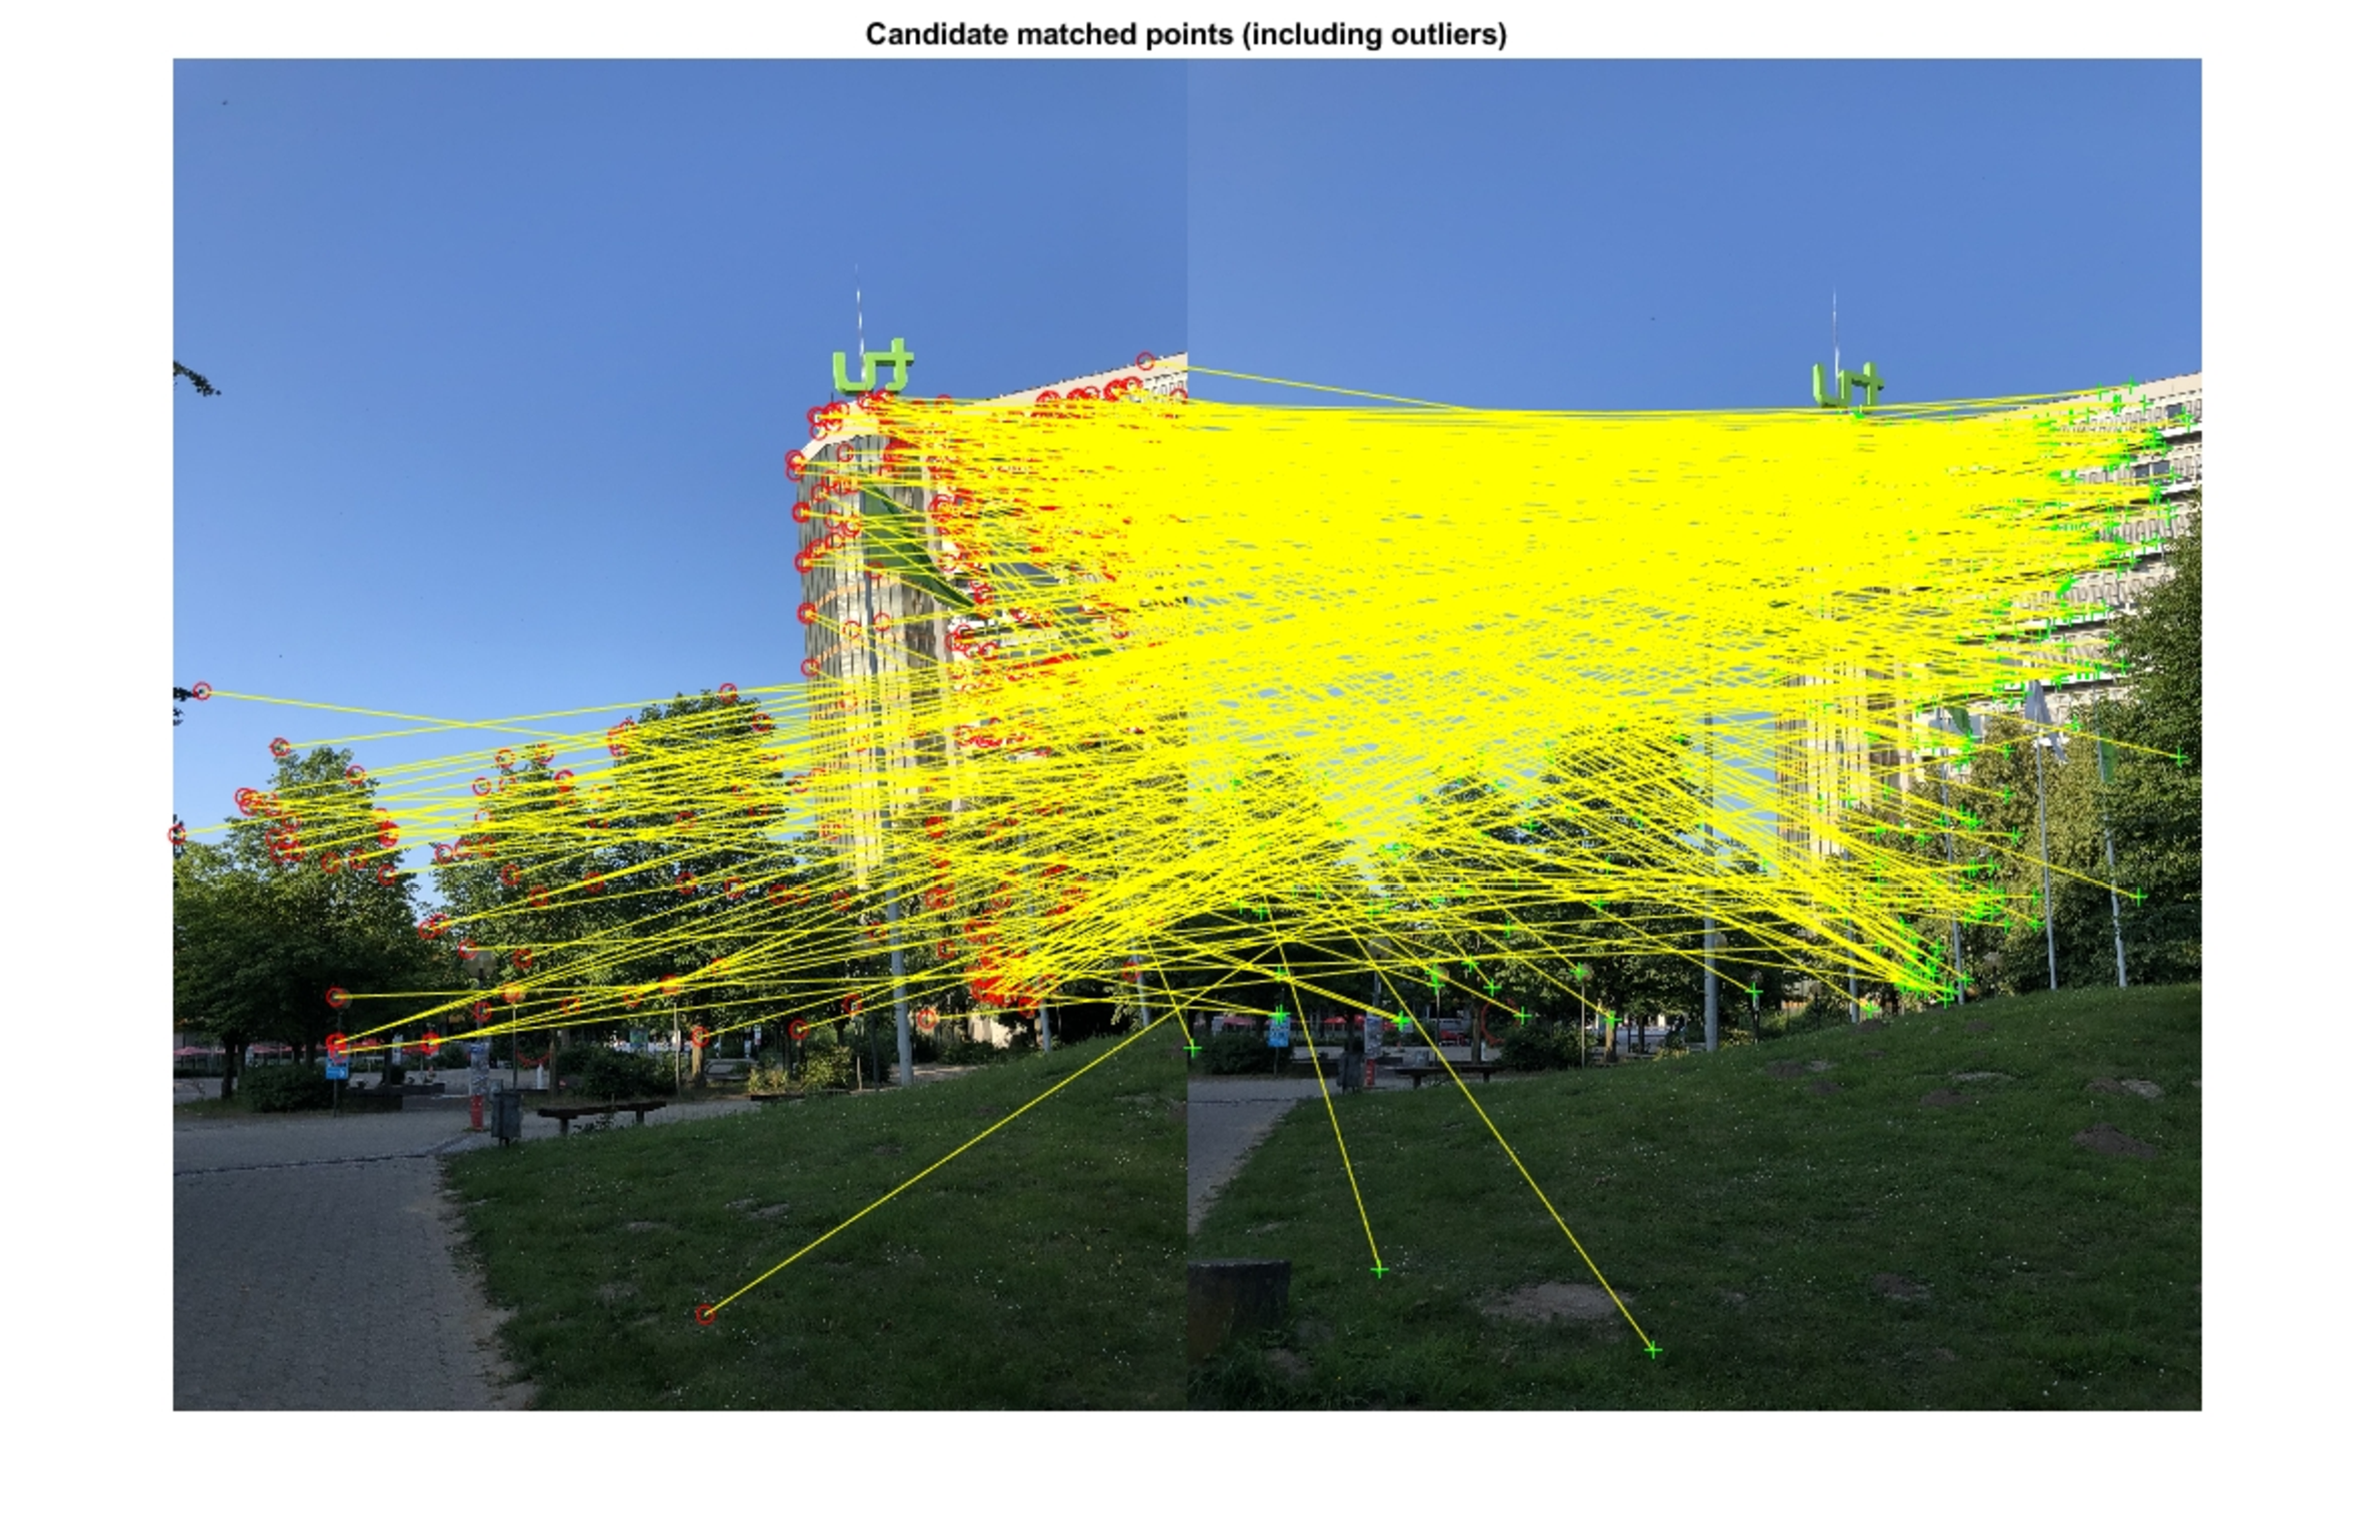
\includegraphics[keepaspectratio,width=0.9\textwidth]{images/4_ZweiteErfahrung/RANSAC/OhneRANSAC.pdf}
 \caption{OhneRANSAC}
 \label{fig:OhneRANSAC}
\end{figure} 

\begin{figure}[H]
 \centering 
 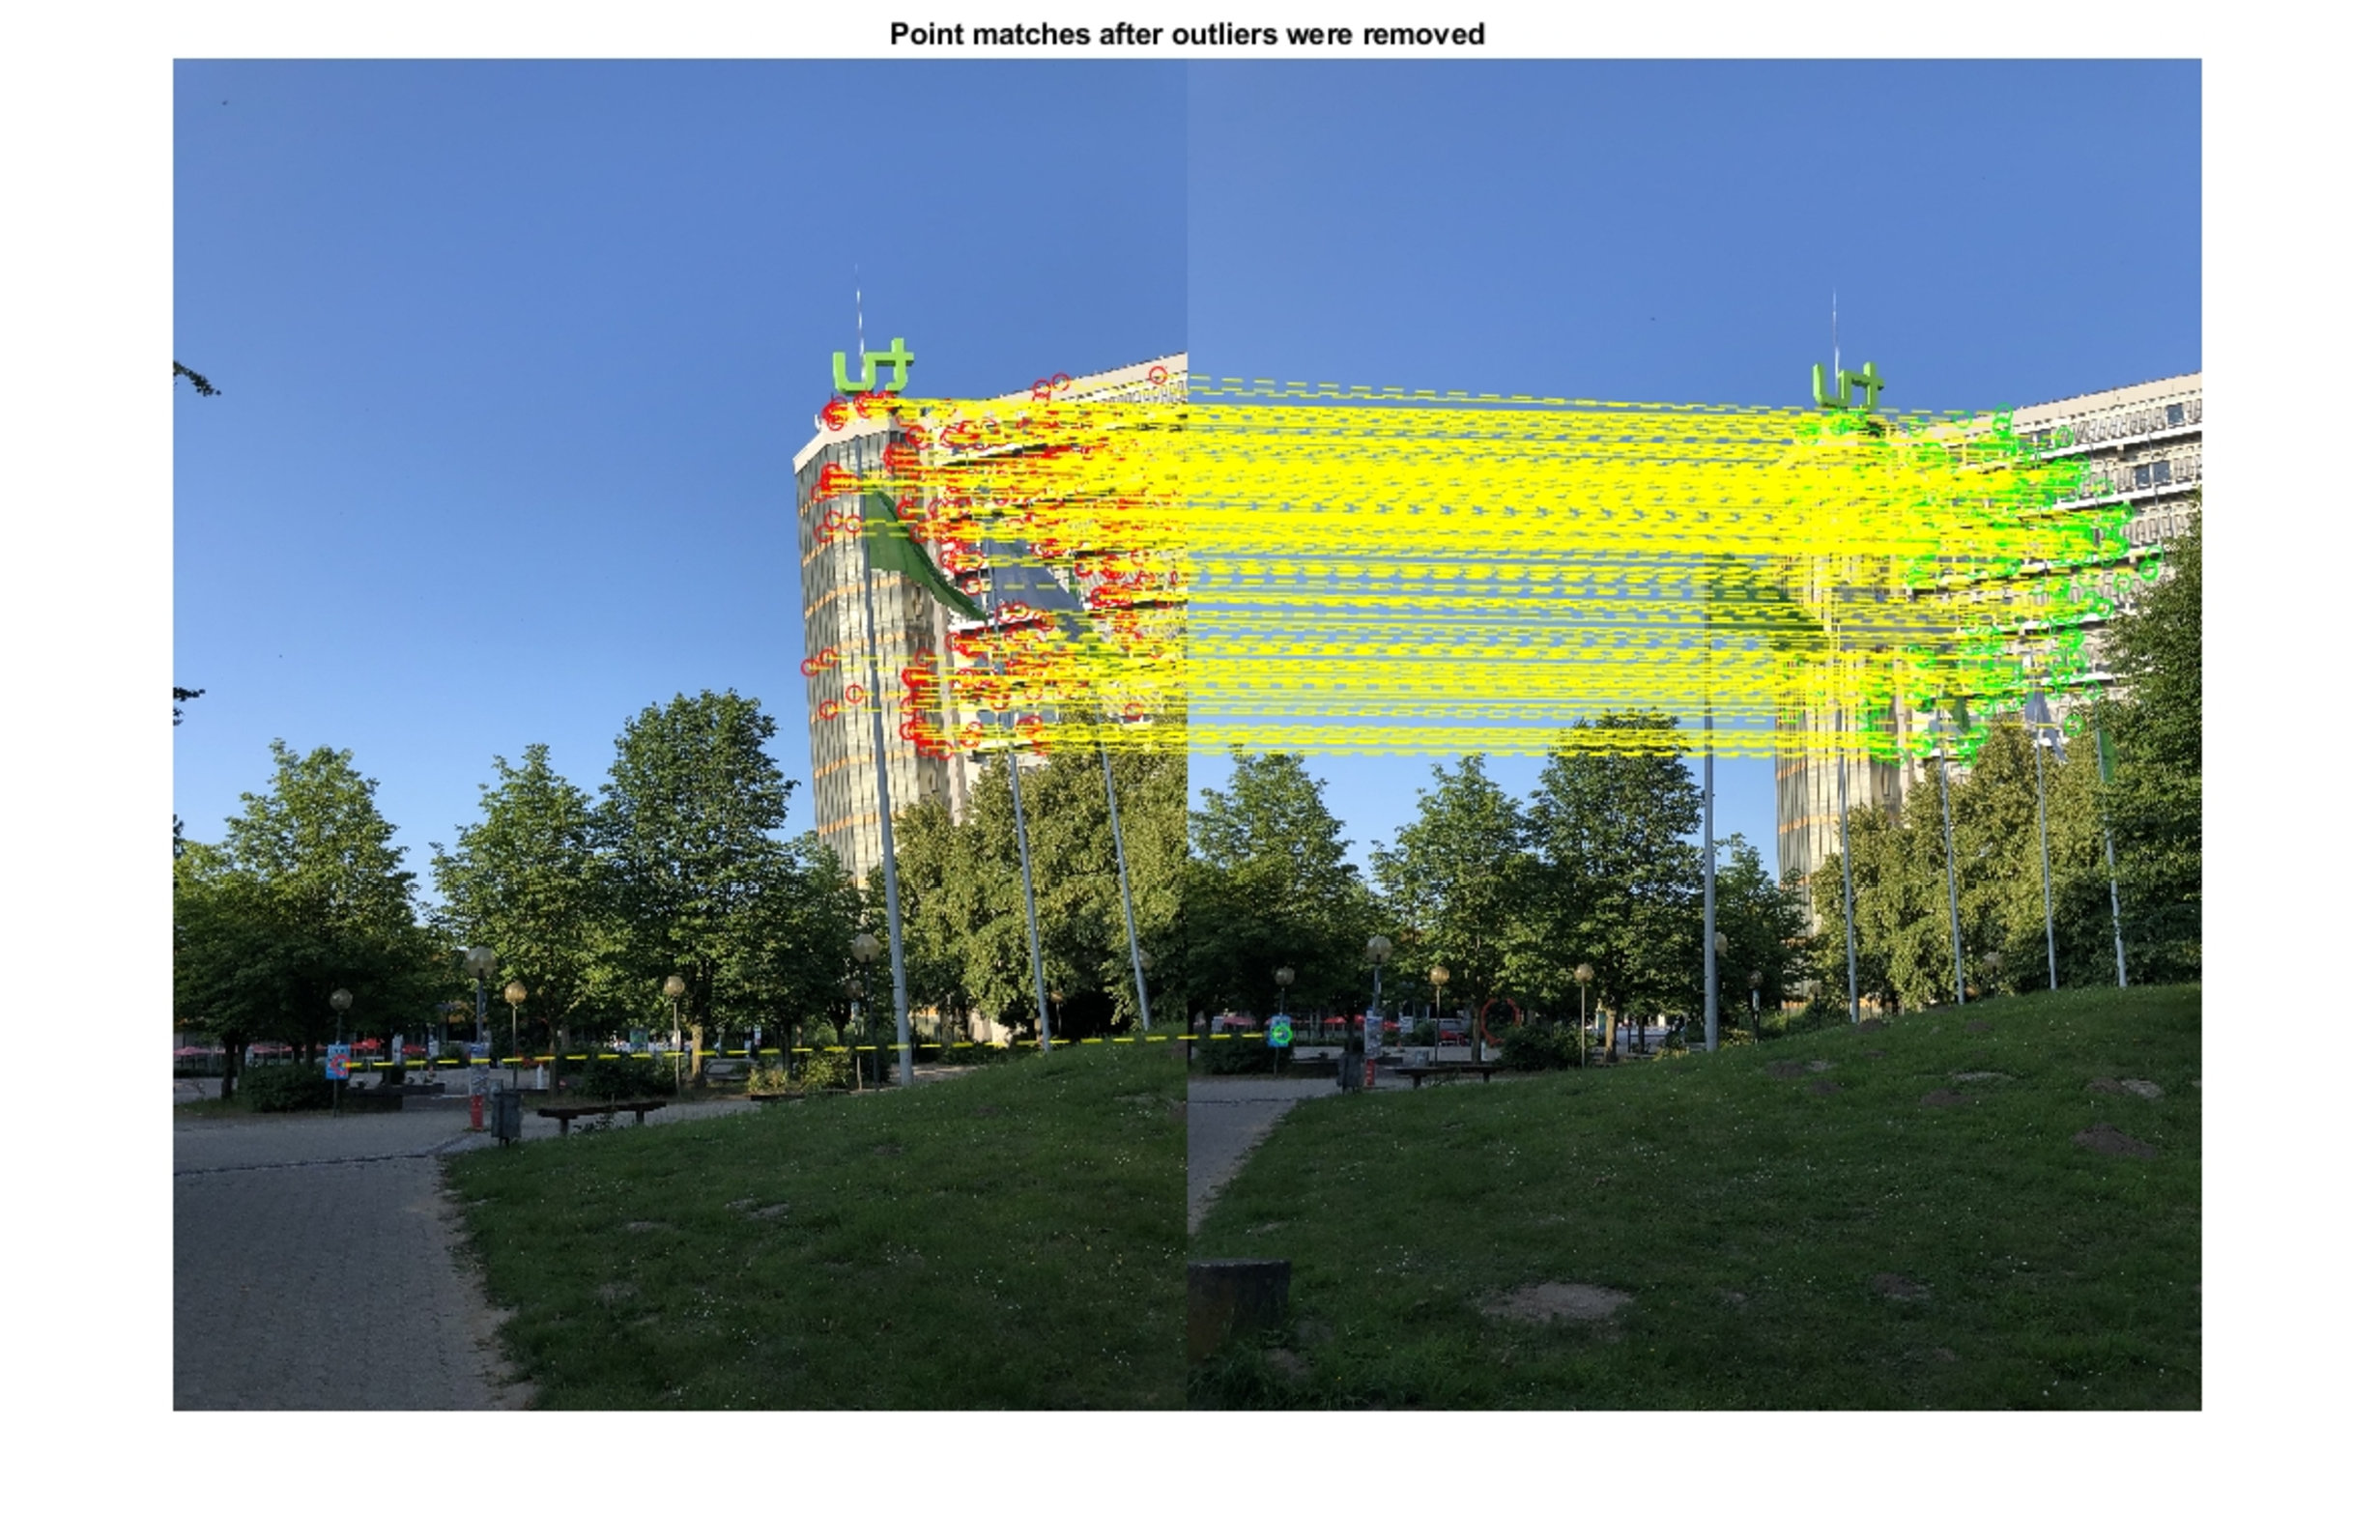
\includegraphics[keepaspectratio,width=0.9\textwidth]{images/4_ZweiteErfahrung/RANSAC/MitRANSAC.pdf}
 \caption{MitRANSAC}
 \label{fig:MitRANSAC}
\end{figure} 


\subsection{Kamerakalibrierung}

Wie in den ersten beiden Abschnitten vorgestellt, finde die übereinstimmende Punkte mit Verwenden des SURF in aufeinanderfolgenden Bildern, dann durch RANSAC lassen die Ausreißer verwerfen. Als nächstes soll die Kamera kalibriert werden, um die Punkte über den zwei Bildern in dasselbe Koordinatensystem konvertieren. In diesem Abschnitt wird zuerst das Kameramodell vorstellt.

\textbf{Kamera Model}

Das Modell der Lochkamera ist in Abbildung 4.10 dargestellt. In dem Modell ist C das optische Zentrum (Fokus), f ist die Kamerabrennweite.

\begin{figure}[htb]
 \centering 
 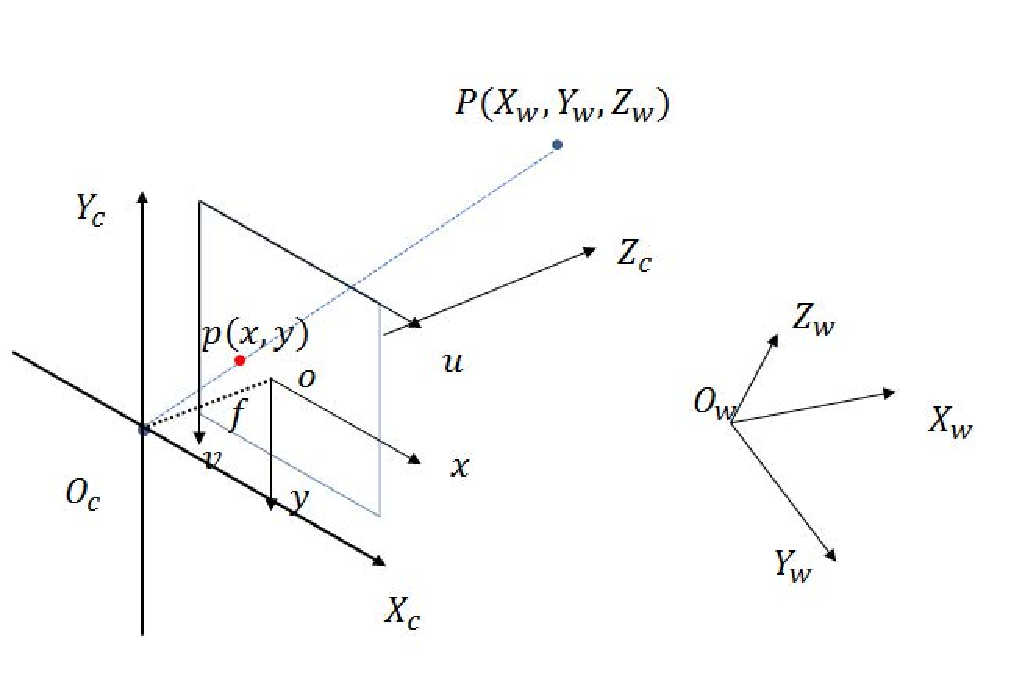
\includegraphics[keepaspectratio,width=0.8\textwidth]{images/4_ZweiteErfahrung/Kamera/cameramodel.pdf}
 \caption{Kamera Model}
 \label{fig:cameramodel}
\end{figure} 

Die vier Koordinatensysteme im Modell sind wie folgt definiert:

\begin{itemize}
	\item 3D Weltkoordinatensystem $W(X,Y,Z)$ \\
	Punktkoordinaten werden durch homogene Koordinaten dargestellt: $\widetilde{X_w}\sim(X_w,Y_w,Z_w,1)^T$
	\item 3D Kamerakoordinatensystem $C(X_c,Y_c,Z_c)$\\
	Punktkoordinaten werden durch homogene Koordinaten dargestellt: $\widetilde{X_c}\sim(X_c,Y_c,Z_c,1)^T$
	\item 2D Bildabbildung Koordinatensystem $P(x,y)$\\
	Punktkoordinaten werden durch homogene Koordinaten dargestellt: $\widetilde{x}\sim(x,y,1)^T$
	\item 2D Bildpixel Koordinatensystem $I(u,v)$\\
	Punktkoordinaten werden durch homogene Koordinaten dargestellt: $\widetilde{u}\sim(u,v,1)^T$
\end{itemize}

% note
Unter diesem Modell wird ein 3D-Punkt im Weltkoordinatensystem durch drei Koordinaten den 2D-Bildpixelkoordinaten zugeordnet.

(a). 3D-Weltkoordinatensystem zum 3D-Kamera-Koordinatensystem.

Die Transformation vom Weltkoordinatensystem zum Kamerakoordinatensystem ist eine Starrekörpertransformation, d.h. das Objekt verformt sich nicht und nur durch Rotation und Parallelverschiebung. Diese Transformation wird in Abbildung 4.11 gezeigt. R bedeutet Rotationsmatrix und T ist Translationsmatrix.

\begin{figure}[htb]
 \centering 
 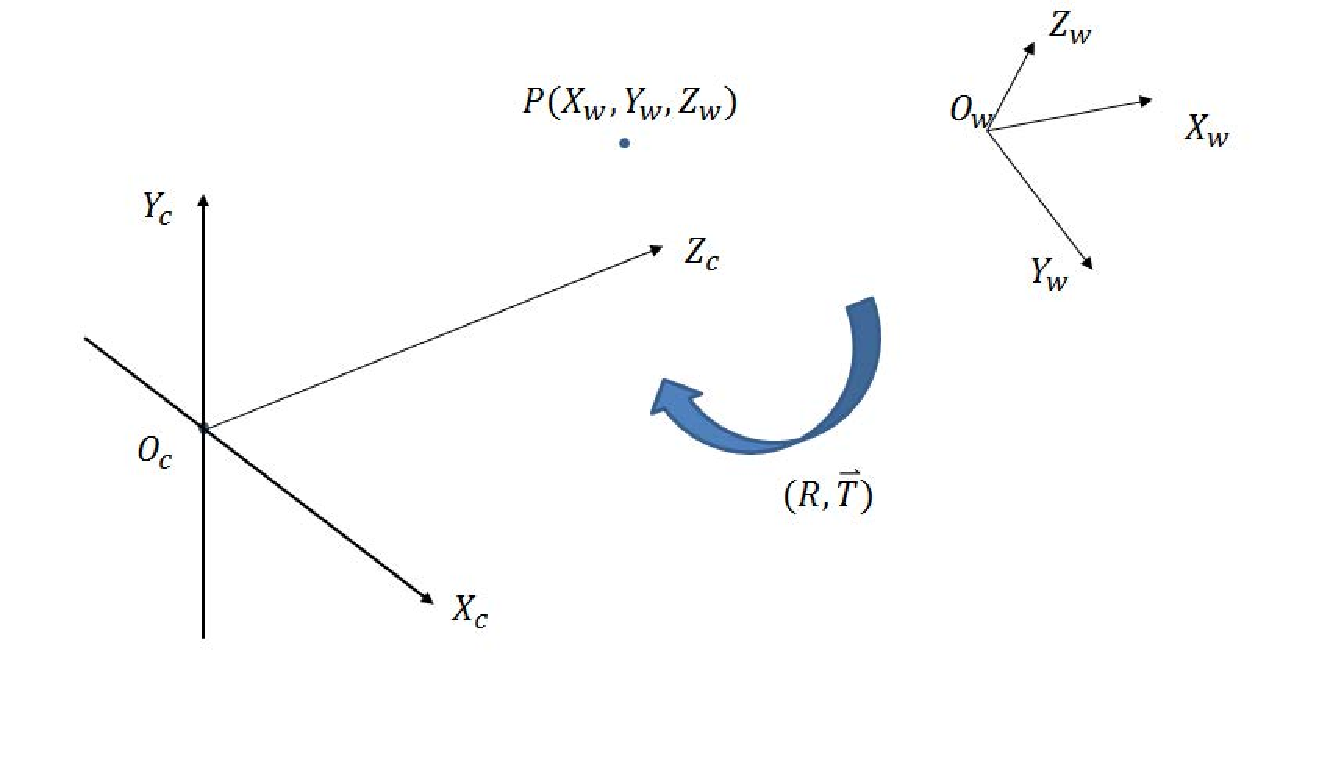
\includegraphics[keepaspectratio,width=0.8\textwidth]{images/4_ZweiteErfahrung/Kamera/WzuC.pdf}
 \caption{Transformation vom Weltkoordinatensystem zum Kamerakoordinatensystem}
 \label{fig:WzuC}
\end{figure} 

Um die entsprechende Rotationsmatrix zu erhalten, wird verschiedene Winkel um verschiedene Koordinatenachsen gedreht. Ein simple Beispiel wird in Abbildung 4.12 gezeigt.

\begin{figure}[H]
 \centering 
 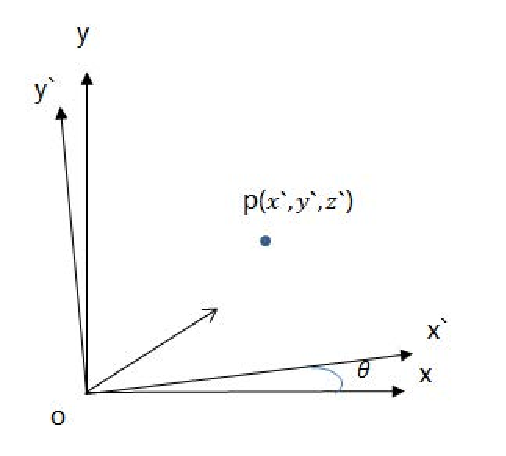
\includegraphics[keepaspectratio,width=0.4\textwidth]{images/4_ZweiteErfahrung/Kamera/rotationsmatrix.pdf}
 \caption{Rotation um Z-Achse}
 \label{fig:rotation}
\end{figure} 

Aus dem Bild können wir leicht bekommen:

\begin{equation}
   \begin{cases} 
	x = x'\cos\theta - y'\sin\theta \\	
	y = x'\sin\theta + y'\cos\theta \\
	z = z'
	\end{cases}
\end{equation}

In Matrixform wie folgend ausgedrückt:

\begin{equation}
   \begin{bmatrix}
	x \\  
	y \\
	z
	\end{bmatrix} = \begin{bmatrix}
	\cos\theta & -\sin\theta & 0	\\
	\sin\theta & \cos\theta  & 0	\\
	0    	   & 0           & 1	
	\end{bmatrix} \cdot \begin{bmatrix}
	x' \\  
	y' \\
	z'
	\end{bmatrix}= R_1 \cdot \begin{bmatrix}
	x' \\  
	y' \\
	z'
	\end{bmatrix}
\end{equation}

In ähnlicher Weise, um die x-Achse, y-Achse dreht sich um $\varphi$ und $\omega$ Grad, bekommen:
\begin{equation}
   \begin{bmatrix}
	x \\  
	y \\
	z
	\end{bmatrix} = \begin{bmatrix}
		1   & 0          & 0	\\
		0   & \cos\varphi & -\sin\varphi	\\
	    0   & \sin\varphi& \cos\varphi	
	\end{bmatrix} \cdot \begin{bmatrix}
	x' \\  
	y' \\
	z'
	\end{bmatrix}= R_2 \cdot \begin{bmatrix}
	x' \\  
	y' \\
	z'
	\end{bmatrix}
\end{equation}

\begin{equation}
   \begin{bmatrix}
	x \\  
	y \\
	z
	\end{bmatrix} = \begin{bmatrix}
	\cos\omega  & 0           & \sin\omega	\\		
	0    	    & 1           & 0	\\
	-\sin\omega &0            &  \cos\omega
	\end{bmatrix} \cdot \begin{bmatrix}
	x' \\  
	y' \\
	z'
	\end{bmatrix}= R_3 \cdot \begin{bmatrix}
	x' \\  
	y' \\
	z'
	\end{bmatrix}
\end{equation}

Dann können die Rotationsmatrix erhalten werden:
\begin{equation}
   R = R_1 \cdot R_2 \cdot R_3
\end{equation}

Kombinieren das Obige, können die Koordinaten von Punkt P im Kamerakoordinatensystem erhalten.
\begin{equation}
   \begin{bmatrix}
	X_C \\  
	Y_c \\
	Z_c
	\end{bmatrix} = R \cdot \begin{bmatrix}
	X_w \\  
	Y_w \\
	Z_w 
	\end{bmatrix} +T
\end{equation}

Im homogenen Koordinatensystem darstellt:
\begin{equation}
   \begin{bmatrix}
	X_C \\  
	Y_C \\
	Z_C \\
	1
	\end{bmatrix} = \begin{bmatrix}
	R & t	\\
	\vec{0}	& 1 \\
	\end{bmatrix} \cdot \begin{bmatrix}
	X_w \\  
	Y_w \\
	Z_w \\
	1
	\end{bmatrix}
\end{equation}

(b). 3D-Kamera-Koordinatensystem zum 2D-Bildabbildung Koordinatensystem.

Die Transformation vom Kamerakoordinatensystem zum Bildkoordinatensystem gehört zur perspektivischen Projektionsbeziehung von 3D zu 2D, wie zeigt in Abbildung 4.13.

\begin{figure}[H]
 \centering 
 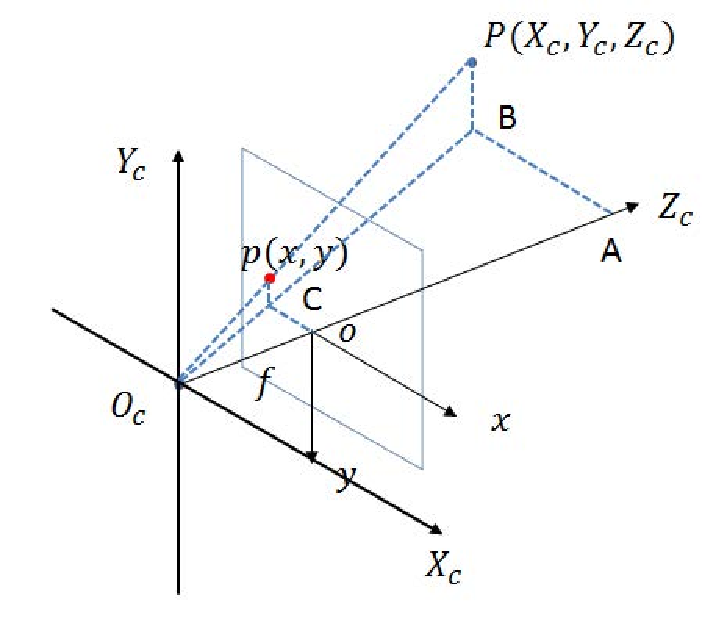
\includegraphics[keepaspectratio,width=0.4\textwidth]{images/4_ZweiteErfahrung/Kamera/Czuimage.pdf}
 \caption{Transformation vom Kamerakoordinatensystem zum Bild Koordinatensystem}
 \label{fig:Czuimage}
\end{figure} 

Es gibt zwei Paare ähnlichen Dreiecken:
\begin{equation}
   \begin{split}
    \triangle ABO_C \sim \triangle oCO_c\\  
	\triangle PBO_C \sim \triangle pCO_c
	\end{split}
\end{equation}

Aus ähnlichen Dreiecksbeziehungen können diese Gleichung Verfügbar sein:
\begin{equation}
   \frac{AB}{oC} = \frac{AO_C}{oO_C} = \frac{PB}{pC} = \frac{X_C}{x} = \frac{Z_C}{f} = \frac{Y_C}{y} 
\end{equation}

Durch die Gleichung Transformation können es erhalten: 
\begin{equation}
   x = f \cdot \frac{X_C}{Z_C}, y = f \cdot \frac{Y_C}{Z_C}
\end{equation}

Im homogenen Koordinatensystem darstellt:
\begin{equation}
   Z_C \cdot \begin{bmatrix}
	x \\  
	y \\
	1
	\end{bmatrix} = \begin{bmatrix}
	f & 0 & 0 & 0	\\
	0 & f & 0 & 0	\\
	0 & 0 & 1 & 0	
	\end{bmatrix} \cdot \begin{bmatrix}
	X_C \\  
	Y_C \\
	Z_C \\
	1
	\end{bmatrix}
\end{equation}

Zu dieser Zeit ist die Einheit des Projektionspunkts p noch nicht Pixel, sondern mm und muss weiter in das Pixelkoordinatensystem umgewandelt werden.

(c). 2D-Bildabbildung Koordinatensystem zum 2D-Bildpixel Koordinatensystem.

Das Pixelkoordinatensystem und das Bildkoordinatensystem befinden sich alle auf der Abbildungsebene, aber die jeweiligen Ursprünge und Maßeinheiten sind unterschiedlich. Der Ursprung des Bildkoordinatensystems ist der Schnittpunkt der optischen Achse der Kamera und der Abbildungsebene, üblicherweise der Mittelpunkt der Abbildungsebene oder der Hauptpunkt. Die Einheit des Bildkoordinatensystems ist mm, die zu der physikalischen Einheit gehört, und die Einheit des Pixelkoordinatensystems ist Pixel. Wir beschreiben gewöhnlich, dass ein Pixel welche Zeilen und Spalten ist. So ist der Übergang zwischen den beiden wie folgt in Abbildung 4.14. 

\begin{figure}[htb]
 \centering 
 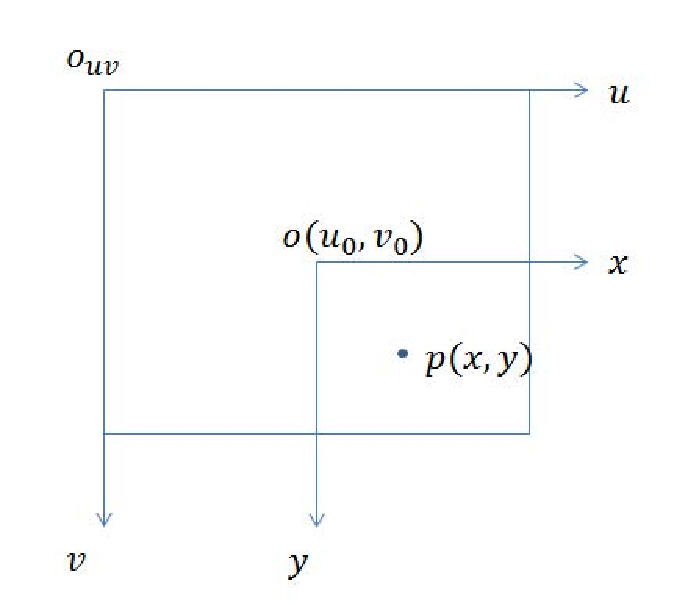
\includegraphics[keepaspectratio,width=0.6\textwidth]{images/4_ZweiteErfahrung/Kamera/imagezupixel.pdf}
 \caption{Konvertierung von Bildkoordinatensystem zu Pixelkoordinatensystem}
 \label{fig:Konvertierung von Pixelkoordinatensystem zu Bildkoordinatensystem}
\end{figure} 

Hier dx, dy ist die Größe jedes Pixels in den X- und Y-Achsenrichtungen. Jedes Pixel des Bildes hat die folgende Beziehung 4.7 in zwei Koordinatensystemen.

\begin{equation}
   \begin{cases} 
	u = \frac{x}{d_x} + u_0	 \\  
	v = \frac{y}{d_y} + v_0	
	\end{cases}
\end{equation}

Im homogenen Koordinatensystem darstellt:

\begin{equation}
   \begin{bmatrix}
	u \\  
	v \\
	1
	\end{bmatrix} = \begin{bmatrix}
	\frac{1}{d_x} 			& 0 			& u_0	\\
	0	 					& \frac{1}{d_y} & v_0	\\
	0     					& 0 			& 1	
	\end{bmatrix} \cdot \begin{bmatrix}
	x \\  
	y \\
	1
	\end{bmatrix}
\end{equation}

Das Bildkoordinatensystem ist eine zweidimensionale Ebene(Bildebene). Es ist in praktisch die Oberfläche des Kamera-CCD-Sensors. Jeder CCD-Sensor hat eine bestimmte Größe und eine bestimmte Auflösung. Diese beide bestimmt die Konvertierungsbeziehung. Eine simple Beispiel, eine Größe des CCD-Sensors ist $\SI{8}{\mm} \times \SI{6}{\mm}$ , die Auflösung dafür ist $640 \times 480$, dann die Beziehung zwischen mm und Pixel läuft $80~pixel/mm$. Lassen Sie die physikalische Größe jedes Pixels des CCD-Sensors $d_x \times d_y$ sein, entspricht läuft $d_x = d_y = \SI{1/80}{\mm}$.
 
Dann durch die Umwandlung der obigen vier Koordinatensysteme kann ein Punkt vom Weltkoordinatensystem zum Pixelkoordinatensystem erhalten.
\begin{equation}
\begin{split}
   Z_C \cdot \begin{bmatrix}
	u \\  
	v \\
	1
	\end{bmatrix} & = \begin{bmatrix}
	\frac{1}{d_x} 			& 0 			& u_0	\\
	0	 					& \frac{1}{d_y} & v_0	\\
	0     					& 0 			& 1	
	\end{bmatrix} \cdot \begin{bmatrix}
	f & 0 & 0 & 0	\\
	0 & f & 0 & 0	\\
	0 & 0 & 1 & 0	
	\end{bmatrix} \cdot \begin{bmatrix}
	R & t	\\
	\vec{0}	& 1 \\
	\end{bmatrix} \cdot \begin{bmatrix}
	X_w \\  
	Y_w \\
	Z_w \\
	1
	\end{bmatrix} \\
	& = \begin{bmatrix}
	f_x & 0 & u_0 & 0	\\
	0 & f_y & v_0 & 0	\\
	0 & 0 & 1 & 0	
	\end{bmatrix} \cdot \begin{bmatrix}
	R & t	\\
	\vec{0}	& 1 \\
	\end{bmatrix} \cdot \begin{bmatrix}
	X_w \\  
	Y_w \\
	Z_w \\
	1
	\end{bmatrix}
\end{split}	
\end{equation}

Die erste Matrix der rechten Gleichung ist die allgemein bekannt interne Referenz der Kamera. Dagegen ist die zweite Matrix die externe Referenz der Kamera. Beide Parameter der Kamera durch Zhang Zhengyou \cite{zhangzhengyou} Kalibrierung erhalten werden. Einige typisch Kamera Parameter von Manufaktur liegt in Tabellen 4.1.

\begin{table}[htb]
	\captionabove{Parameter des Kameras im Vergleich}
	\label{tbl:params}
	\footnotesize
	\centering
	\rowcolors{2}{white}{gray!25}	%TUgreen!25
	\begin{tabular}{|p{3cm}|p{2.5cm}|p{2.5cm}|p{2.5cm}|}	%p{}m{}b{}clr
	\toprule
	\textbf{Parameter} & \textbf{Google Pixel} & \textbf{Google Pixel2} & \textbf{Iphone 10}\\
	\midrule
	Sensor Größe $''$ & 1/2.3 & 1/2.6 & 1/3 \\
	Bild Auflösung $pixels$ & $4048 \times 3036$ & $4032 \times 3024$ & $4032 \times 3024$ \\
	Pixel Größe $\mu m$ & 1.544 & 1.4 & 1.22 \\	
	Brennweite $mm$ & 4.67 & 4.47 & 3.99 \\
	Formatfaktor $35 mm$  	&5.55	&6.04	&7.02	\\
	
	\bottomrule
	\end{tabular}
\end{table} 


Aus der obigen Formel wenn die internen und externen Parameter der Kamera bekannt sind, ist nämlich die Projektionsmatrix bekannt, und zu diesem Zeitpunkt können die entsprechenden Bildkoordinaten für jeden beliebigen räumlichen Punkt erhalten werden. Dagegen  wenn die Position m (u, v) in Bildkoordinate bekannt ist, und auch die Parameter innerhalb und außerhalb der Kamera bereits bekannt sind, kann die entsprechenden Punkt in Wert Koordinate nicht eindeutig bestimmt werden. Die Grund dafür ist, die $Z_c$ Information während des Projektionsprozesses eliminiert wird. 

\textbf{Image Warping}

In diese Arbeit wird zuerst eine vereinfachte Situation  betrachten, d.h. nur mit Rotations Einfluss. Abbildung 4.15 zeigt das 3D-Rotationsbewegungsmodell der Kamera. Die Position des optischen Zentrums ändert sich während der Kamerabewegung im Drehbewegungsmodell der Kamera nicht. Unter diesem Modell ist die Abbildungsbeziehung zwischen dem Punkt X im Weltkoordinatensystem und der Bildkoordinate x im homogenen Koordinatensystem dargestellt: 
\begin{equation}
   x = KRX, X = \lambda  K^{-1} x
\end{equation}

Wobei: K ist der interne Parameter der Kamera, wie zuvor definiert. $\lambda$ ist der unbekannte Skalierungsfaktor, d.h. unter dem Kameramodell die Quelle der Bildpunktkoordinaten einem Strahl zugeordnet ist.

\begin{figure}[htb]
 \centering 
 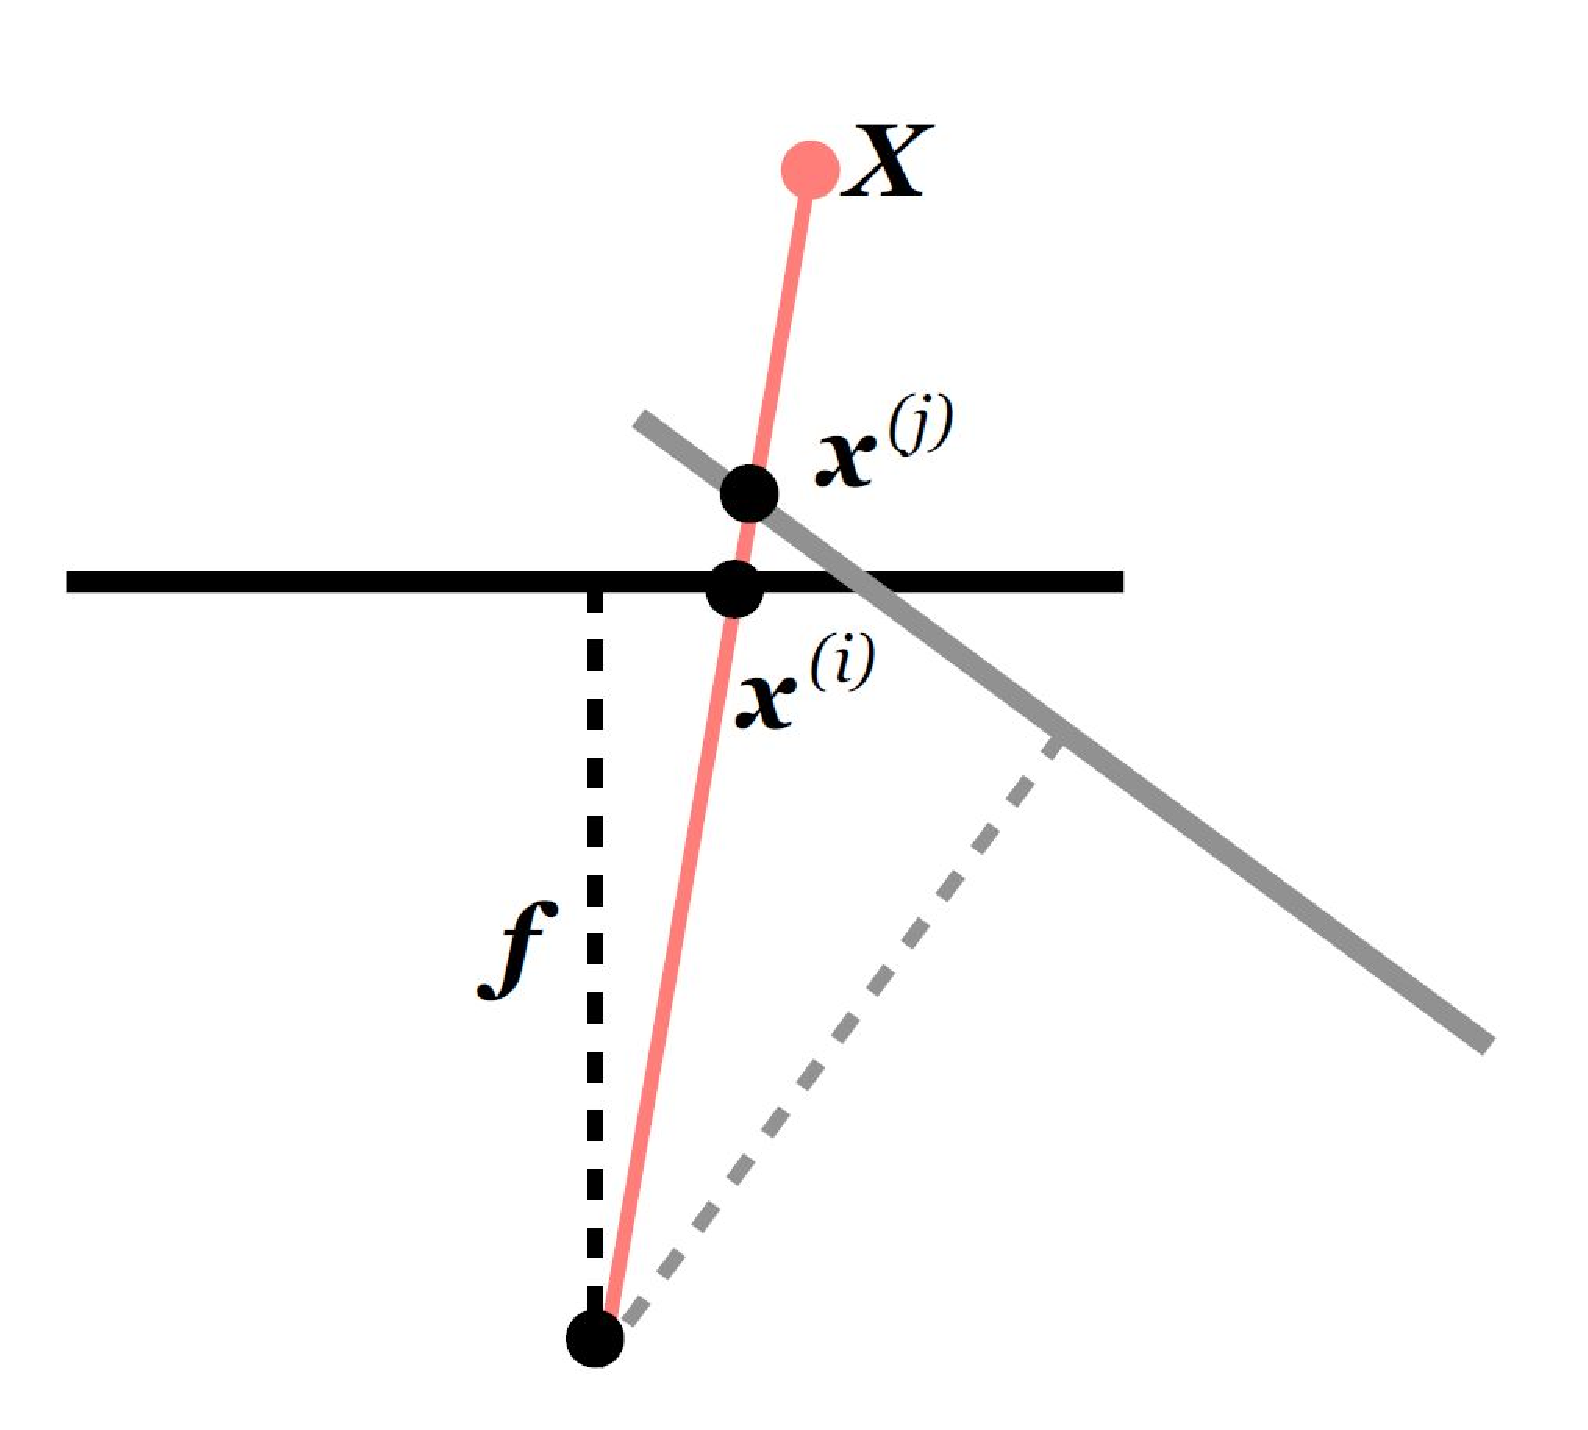
\includegraphics[keepaspectratio,width=0.5\textwidth]{images/4_ZweiteErfahrung/Kamera/rotationsmodel.pdf}
 \caption{Rotationsbewegungsmodell}
 \label{fig:rotationsmodel}
\end{figure} 


Herleiten nun die Beziehung zwischen Bildpunkten in einem Framepaar für zwei verschiedene Kameraausrichtungen (siehe Abbildung 4.15). Für einen Weltkoordinatepunkt X sind die projizierten Punkte $x_i$ und $x_j$ in der Bildebene von zwei Bildern i und j gegeben durch
\begin{equation}
   x_i = KR_iX, x_j = KR_jX
\end{equation}

Anordnen diese Gleichungen weiter und ersetzen X, wird eine Beziehung aller Punkte im Bildrahmen i auf alle Punkte im Rahmen j erhalten:
\begin{equation}
   x_j = KR_jR_i^TK^{-1}x_i
\end{equation}

Bisher wird nur die Beziehung zwischen zwei Bildern desselben Videos betrachtet. Lockern diese Einschränkung, indem Frames von einer Kamera, die sich gemäß $R$ dreht, zu einer anderen Kamera, die sich gemäß $R'$ dreht, abbilden. Es gibt eine Hypothese, dass beide Kamerazentren sich im Ursprung befinden. Dann die Warping-Matrix, die Punkte von einer Kamera auf die andere abbildet, definiert werden können:
\begin{equation}
   W = KR'R^TK^{-1}
\end{equation}

Es wird hier angenommen, dass das erste Bild als Referenz genommen wird und der Rotationswinkel 0 ist. Dann die Gleichung kann vereinfacht werden:
\begin{equation}
   W = KRK^{-1}
\end{equation}

Kombiniert mit Formel 4.23 können es ausgedrückt als:
\begin{equation}
   x_j = Wx_i
\end{equation}

\textbf{Kalibrierung Optimierung}

In diesem Abschnitt wird die Parameter in der Warping-Matrix berechnt. Überprüfen die letzten beiden Abschnitte, mit Verwendung des SURF~\cite{Surf} die übereinstimmende Punkte in aufeinanderfolgenden Bilderrahme entdeckt werden dann durch RANSAC~\cite{ransac1}, Ausreißer verworfen werden. Das Ergebnis ist eine Menge von Punktkorrespondenzen $x_i$ und $x_j$ für alle benachbarten Bilder. Angesichts dieser Grundwahrheit kann man die Kalibrierung als ein Optimierungsproblem formulieren, wobei wir den Fehler bei der Mittelwertbildung im Quadrat aller Punktkorrespondenzen minimieren wollen:
\begin{equation}
   J = \sum_{(i,j)}\lVert x_j - Wx_i \rVert ^2
\end{equation}

Beachten, dass dies ein nichtlineares Optimierungsproblem ist. Einige nichtlinearer Optimierer könnte verwendet werden, um diese Zielfunktion zu minimieren. Jedoch ist es gefunden, dass Koordinatenabstieg durch direkte objektive Funktionsbewertung schnell konvergiert. Jedes Mal, wenn einen Schritt gemacht wird, bei dem die Zielfunktion J nicht abnimmt, kehren die Schrittrichtung um und verringern die Schrittweite des entsprechenden
Parameter. Der Algorithmus endet, sobald die Schrittgröße für alle Parameter unter einen gewünschten Schwellenwert fällt (d.h. Wenn eine Zielgenauigkeit erreicht haben). Das Flussdiagramm des Algorithmus ist wie folgt:

\begin{figure}[H]
 \centering 
 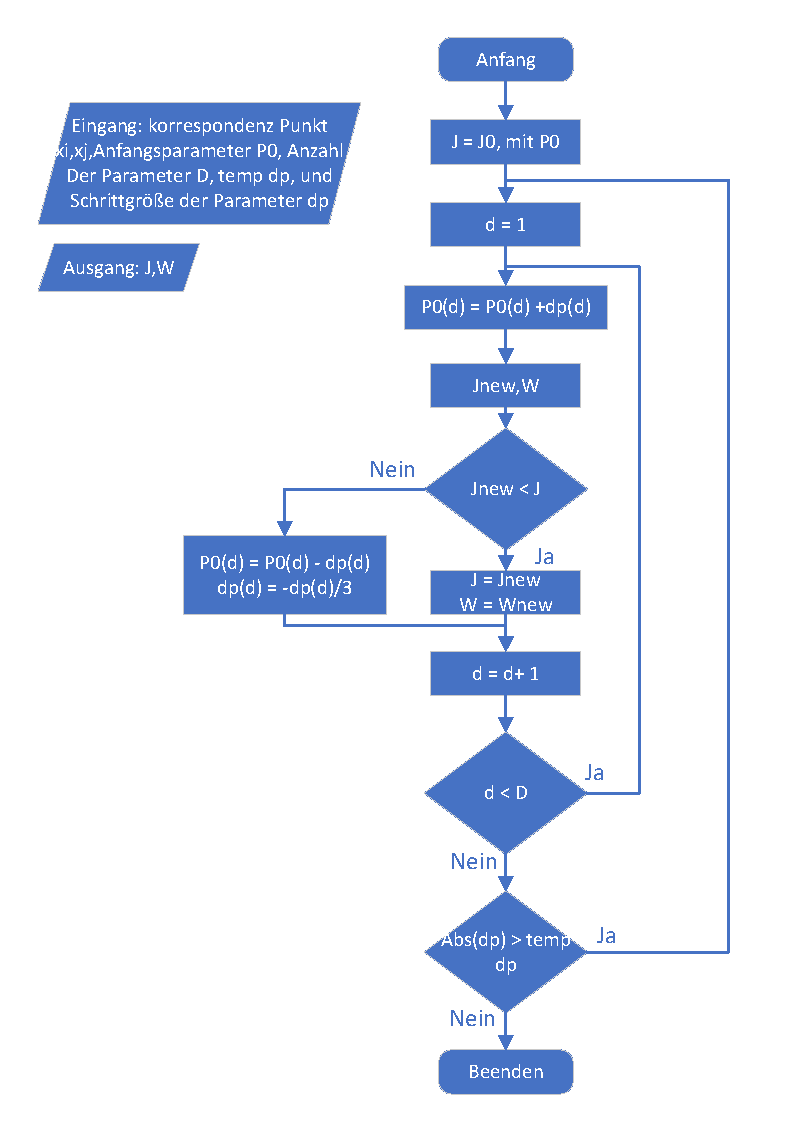
\includegraphics[keepaspectratio,width=0.8\textwidth]{images/4_ZweiteErfahrung/Kamera/flussdiagramm_for_parameter.pdf}
 \caption{Flussdiagramm für Algorithmus}
 \label{fig:rotationsmodel}
\end{figure} 

Weiter in einem allgemeineren Fall, d.h. derzeit nicht nur mit Rotations Einfluss, sondern auch Translations Einfluss nehmen. Das Verlauf ist im Allgemeinen gleich. Der Hauptunterschied ist Anzahl der Parametern, die von original nur 3 Rotationsparameter zur jetzt 6 Parameter einschließlich 3 Rotationsparameter und 3 Translationsparameter. Das neu Warping-Matrix darstellt wie folgen:
\begin{equation}
   W = \begin{bmatrix}
	f			& 0 		& \frac{w}{2}	  & 0 \\
	0	 		& f			& \frac{h}{2} 	  & 0 \\
	0     		& 0 		& 1 			  & 0 \\	
	0     		& 0 		& 0 			  & 1
	\end{bmatrix} \cdot \begin{bmatrix}
	R_{11}			& R_{21}  		& R_{31}	  & 0 \\
	R_{12}	 		& R_{22}		& R_{32}	  & 0 \\
	R_{13}     		& R_{23} 		& R_{33} 	  & 0 \\	
	t1     			& t2 			& t3 		  & 1
	\end{bmatrix} \cdot \begin{bmatrix}
	\frac{1}{f}	   & 0 				& -\frac{w}{2f}	  & 0 \\
	0	 		   & \frac{1}{f}	& -\frac{h}{2f}   & 0 \\
	0     		   & 0 		        & 1 			  & 0 \\	
	0     		   & 0 		        & 0 			  & 1
	\end{bmatrix}
\end{equation}

Dann durch Transformationsmatrix können die Koordinaten des zweiten Bildes in die Koordinaten des ersten Bildes umgewandelt werden. Abbildung 4.17 zeigt diese Verlauf. Die Ergebnisse der beiden experimentellen Fälle werden im nächsten Kapitel detailliert beschrieben. 

\begin{figure}[H]
 \centering 
 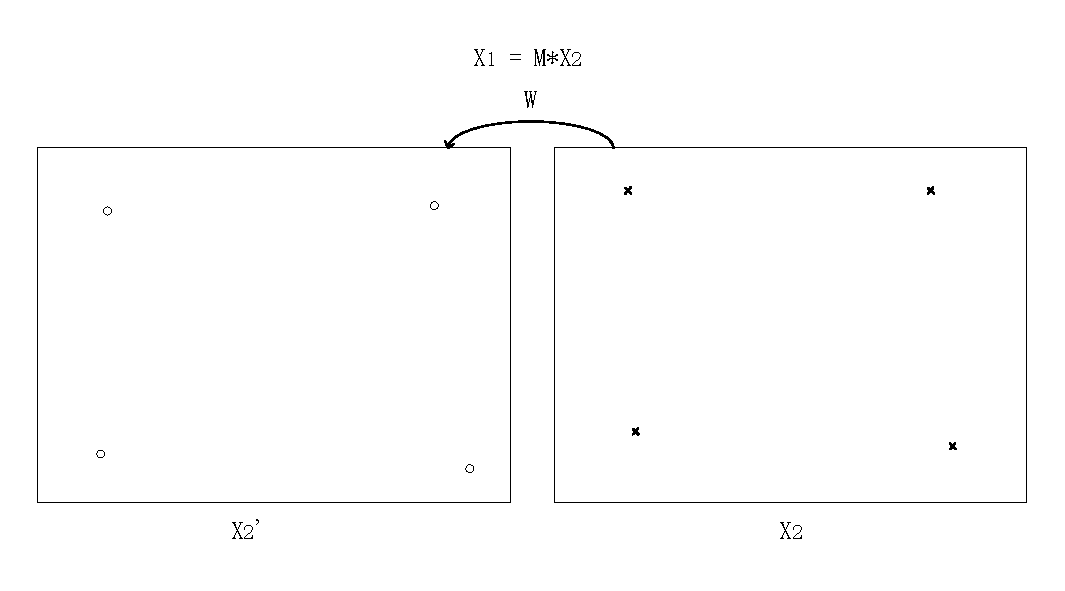
\includegraphics[keepaspectratio,width=0.9\textwidth]{images/4_ZweiteErfahrung/Kamera/Transformmatrix.pdf}
 \caption{Transformation in eine Koordinate}
 \label{fig:Transformation in eine Koordinate}
\end{figure} 

\section{Differenzbild Optimierung}
Durch Bildregistration erhalten eine Reihe Bilder von der Kamera, deren Koordinaten in dasselbe Koordinatensystem umgewandelt wurden. Die Ziel in diesem Abschnitt ist ein detektierendes Bilder herstellen, dadurch die QR Muster Detektion vereinfachen werden können. Auswälen je zwei Bilder und subtrahieren, um eine Reihe Differenzbildern zu enthälten. Es sollte hier beachtet werden, dass aufgrund der Zeitsynchronisation die QR Muster in diesen Differenzbilder die folgende Situation aufgetreten sein können. Nehmen an, dass es in der vertikalen Richtung ist.

\begin{itemize}
	\item total Schwarz-Weiß-Schwarz-Weiß-Schwarz Ordnung.
	\item halb Schwarz-Weiß-Schwarz-Weiß-Schwarz Ordnung, halb nicht gezeigt.
	\item total Weiß-Schwarz-Weiß-Schwarz-Weiß Ordnung.
	\item halb Weiß-Schwarz-Weiß-Schwarz-Weiß Ordnung, halb nicht gezeigt.
	\item halb Schwarz-Weiß-Schwarz-Weiß-Schwarz Ordnung, halb Weiß-Schwarz-Weiß-Schwarz-Weiß Ordnung.
	\item total nicht gezeigt.
\end{itemize}

Tabelle zeigt einige Beispiel.

\begin{table}[htb]
	\captionabove{einige Beispiel}
	\label{tbl:params}
	\footnotesize
	\centering
	\rowcolors{2}{white}{gray!25}	%TUgreen!25
	\begin{tabular}{|p{2cm}<{\centering}|c|p{2cm}<{\centering}|c|}	%p{}m{}b{}clr p{3cm} p{8cm}
	\toprule
	\textbf{Ob angepasst zu folgende Detektion?} & \multirow{4}{*}{\textbf{einige Beispiel}} & \textbf{Ob angepasst zu folgende Detektion?} & \multirow{4}{*}{\textbf{einige Beispiel}} \\
	\midrule
	 Ja & 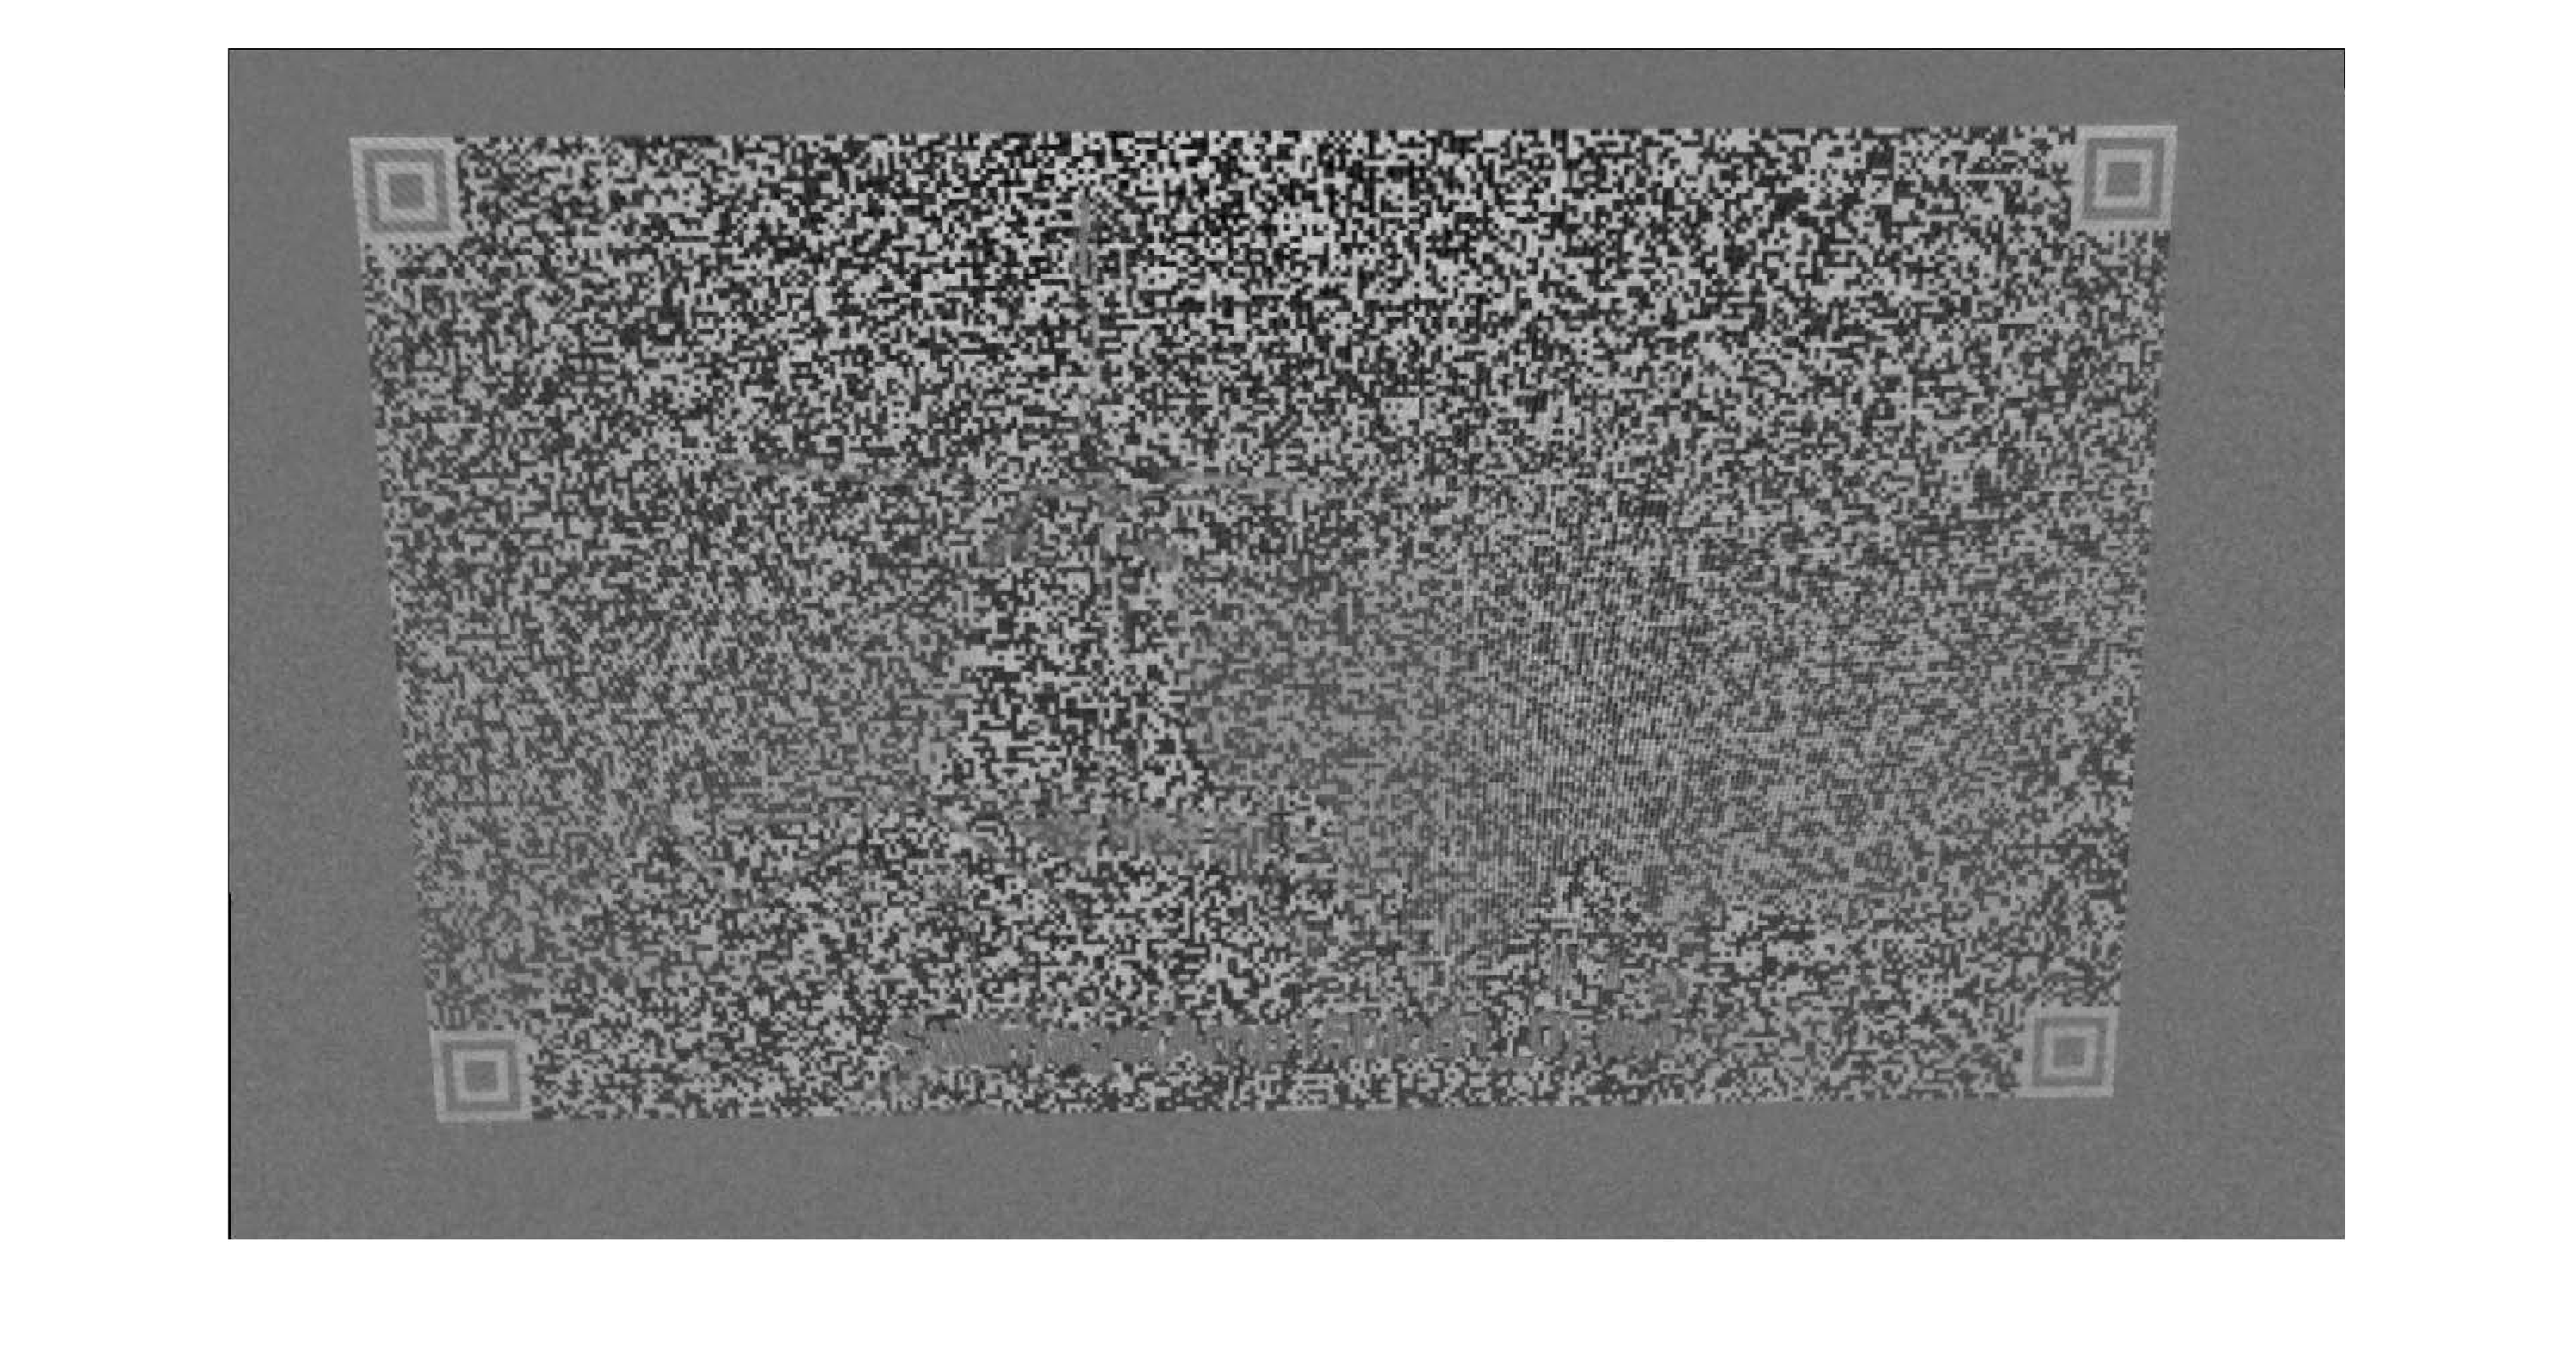
\includegraphics[scale=0.12]{images/4_ZweiteErfahrung/Differenzbild/0schwarz.pdf}& Nein & 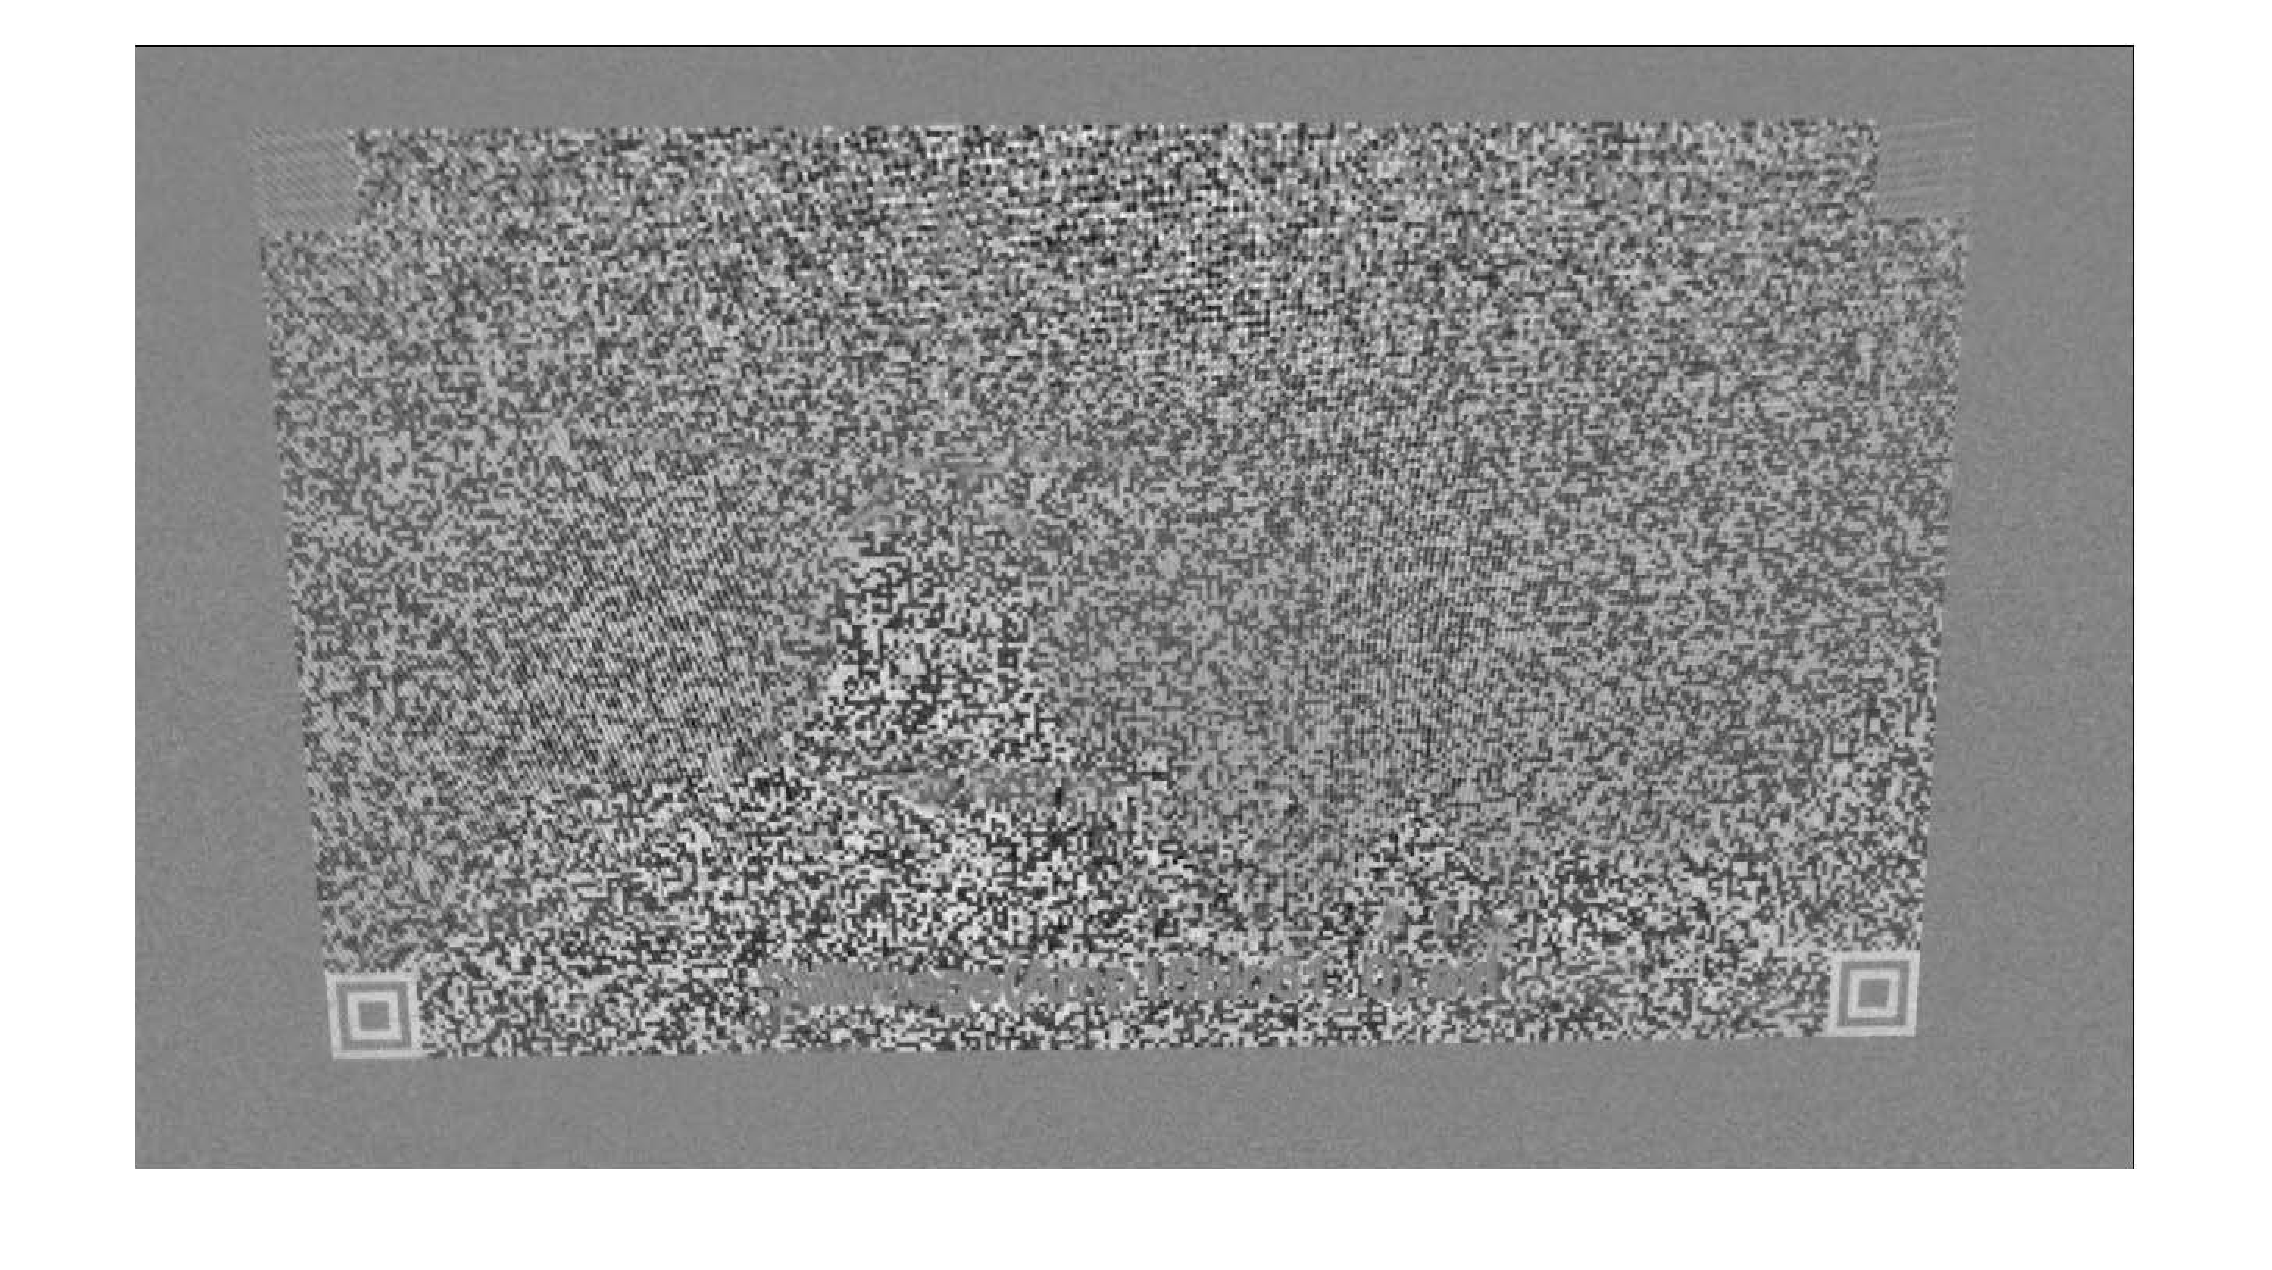
\includegraphics[scale=0.15]{images/4_ZweiteErfahrung/Differenzbild/1halfschwarz.pdf}\\
	Nein & 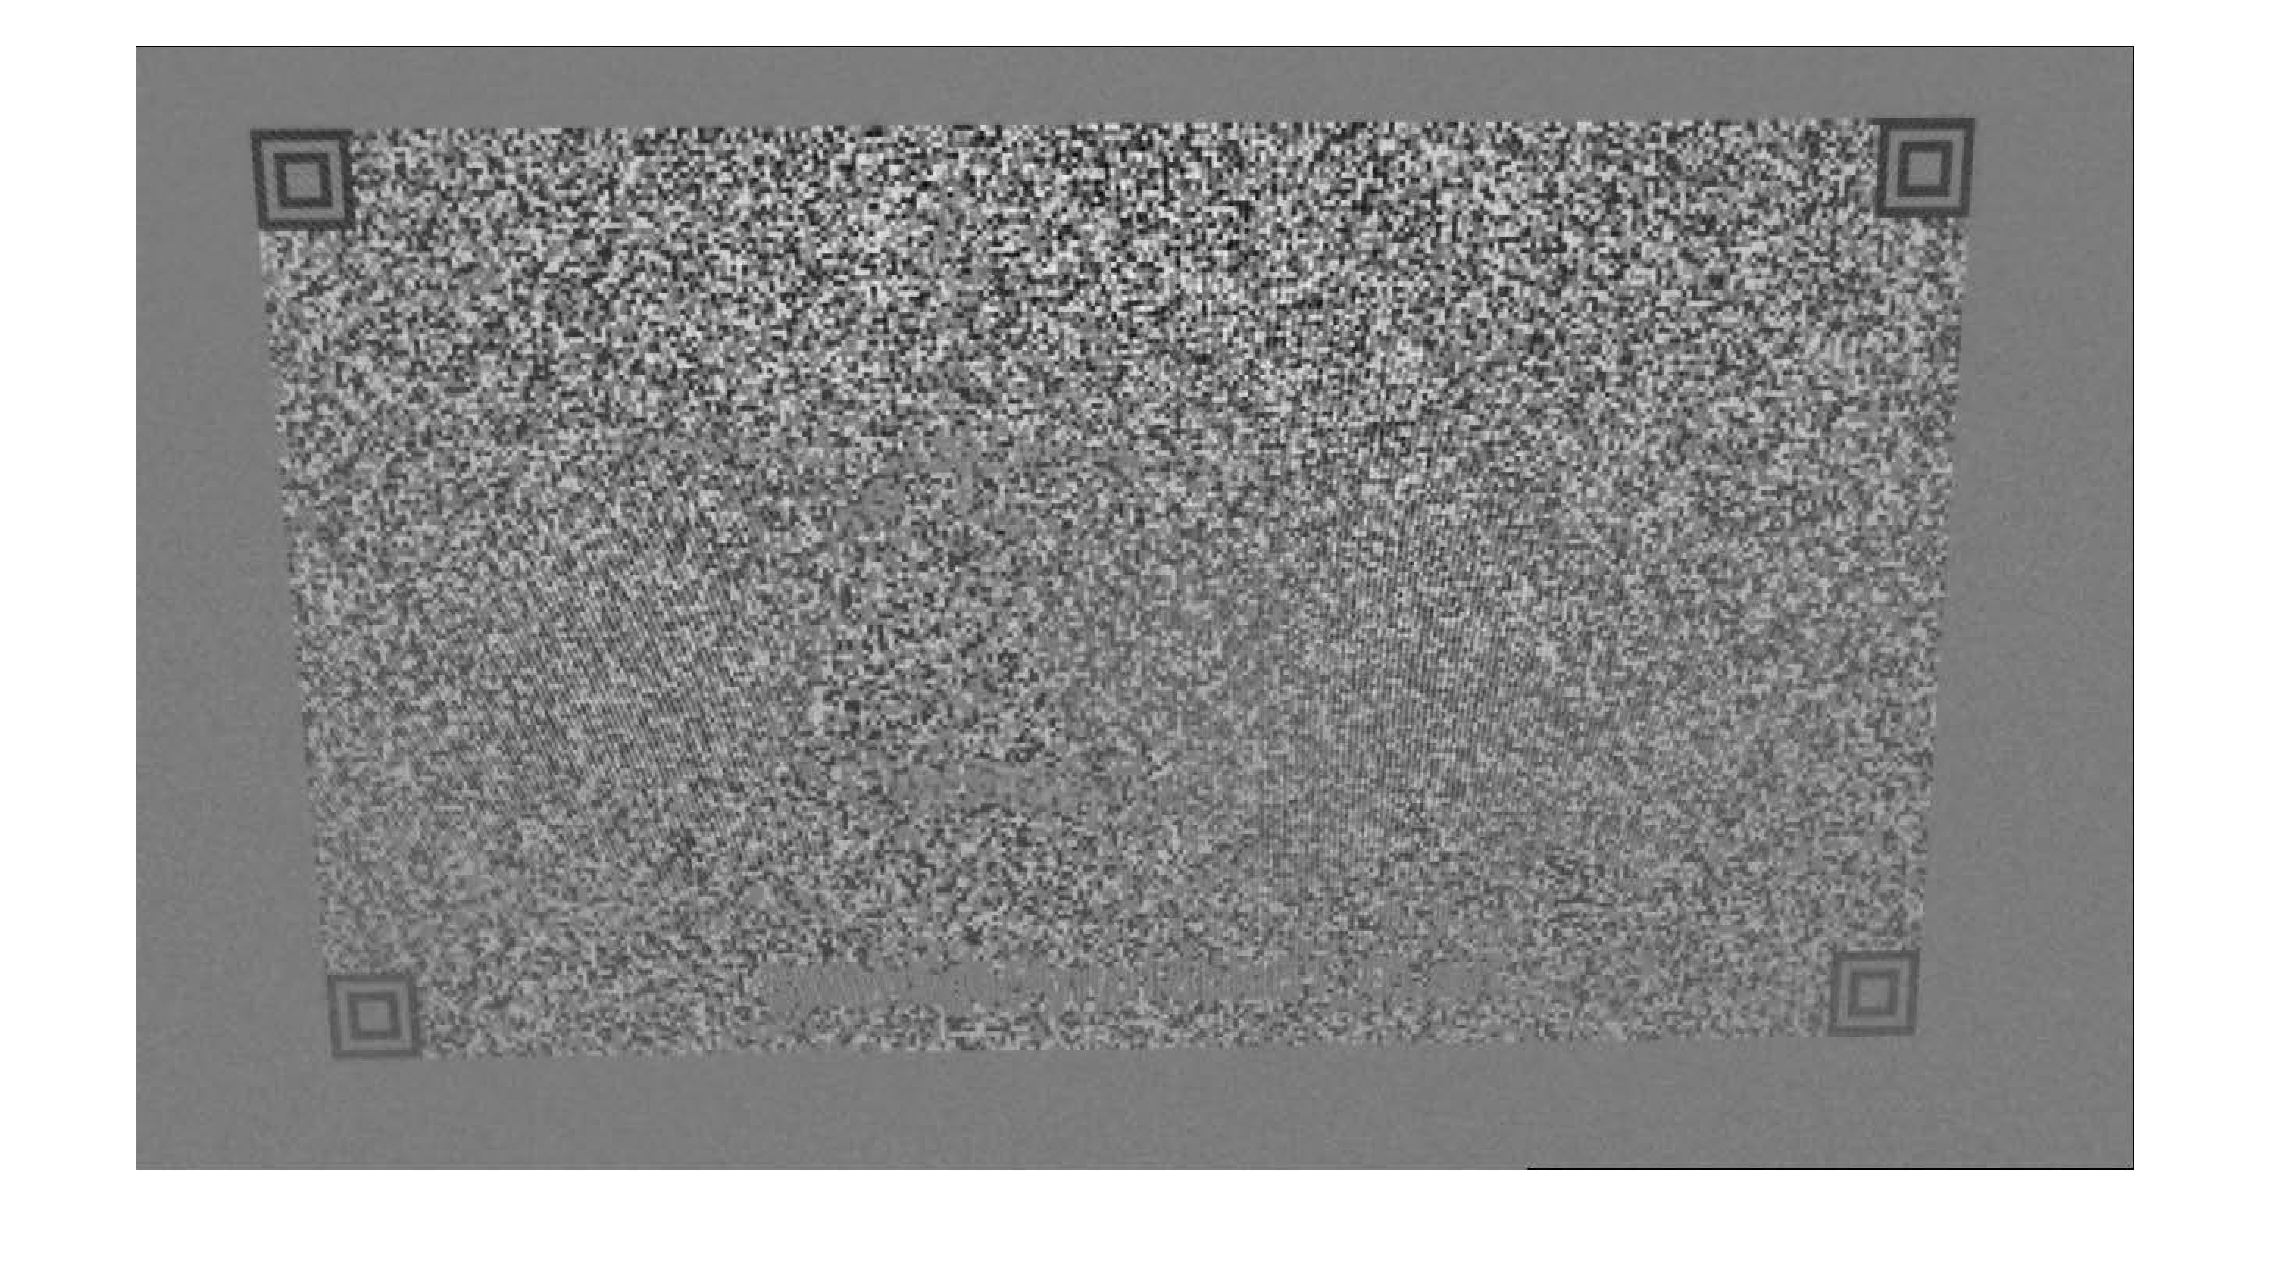
\includegraphics[scale=0.15]{images/4_ZweiteErfahrung/Differenzbild/2weis.pdf}& Nein & 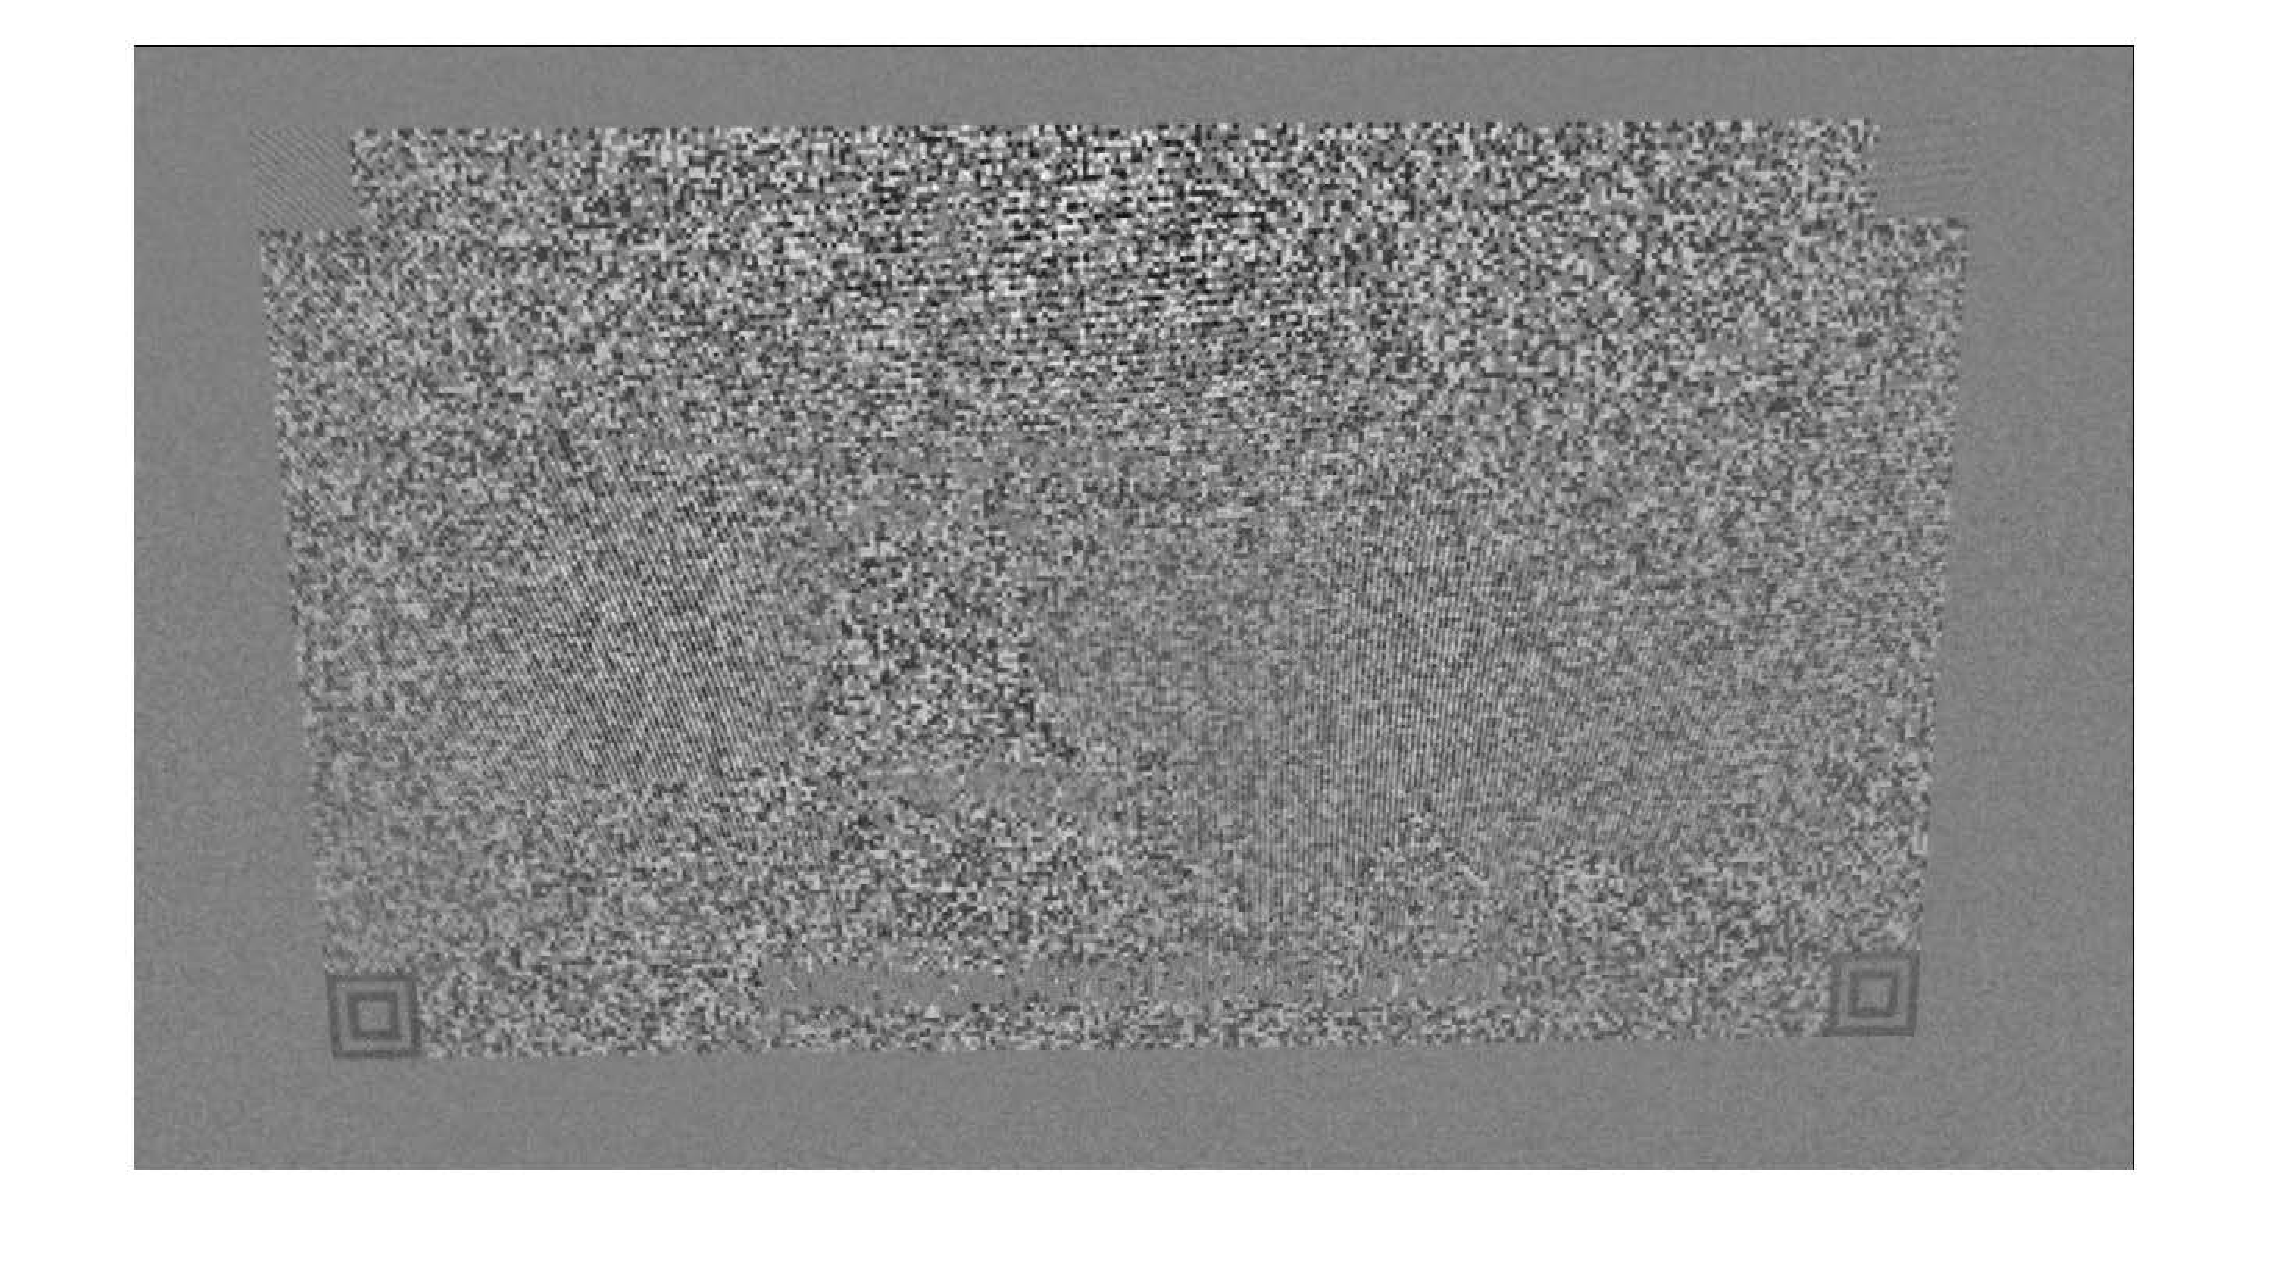
\includegraphics[scale=0.15]{images/4_ZweiteErfahrung/Differenzbild/3halfweis.pdf}\\
	Nein & 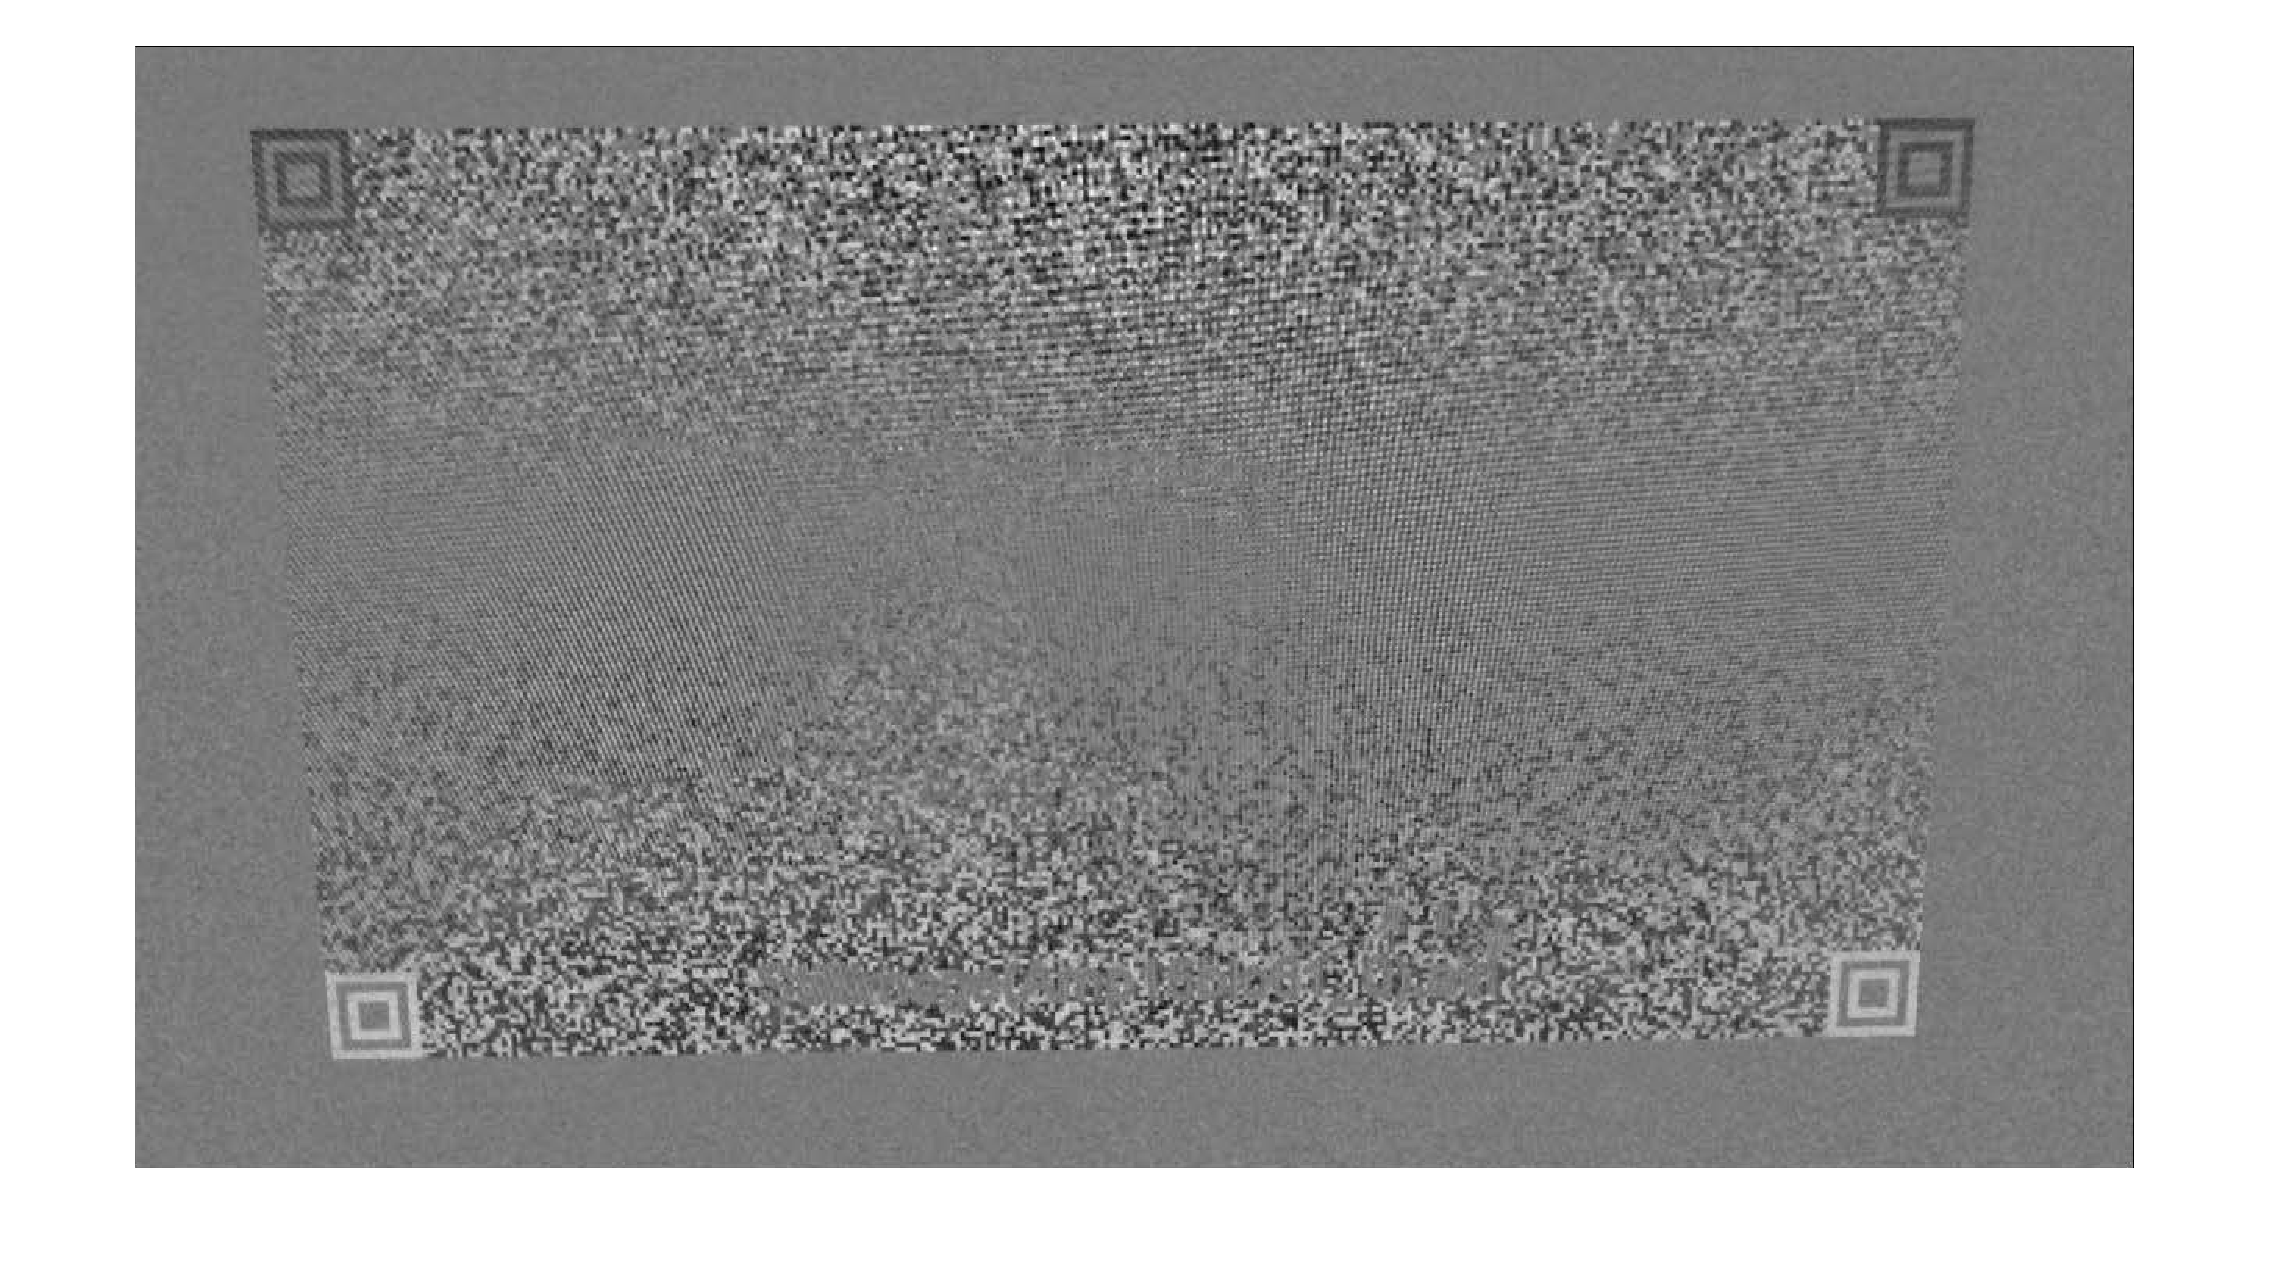
\includegraphics[scale=0.15]{images/4_ZweiteErfahrung/Differenzbild/4halbschwaryhalbweis.pdf}& Nein & 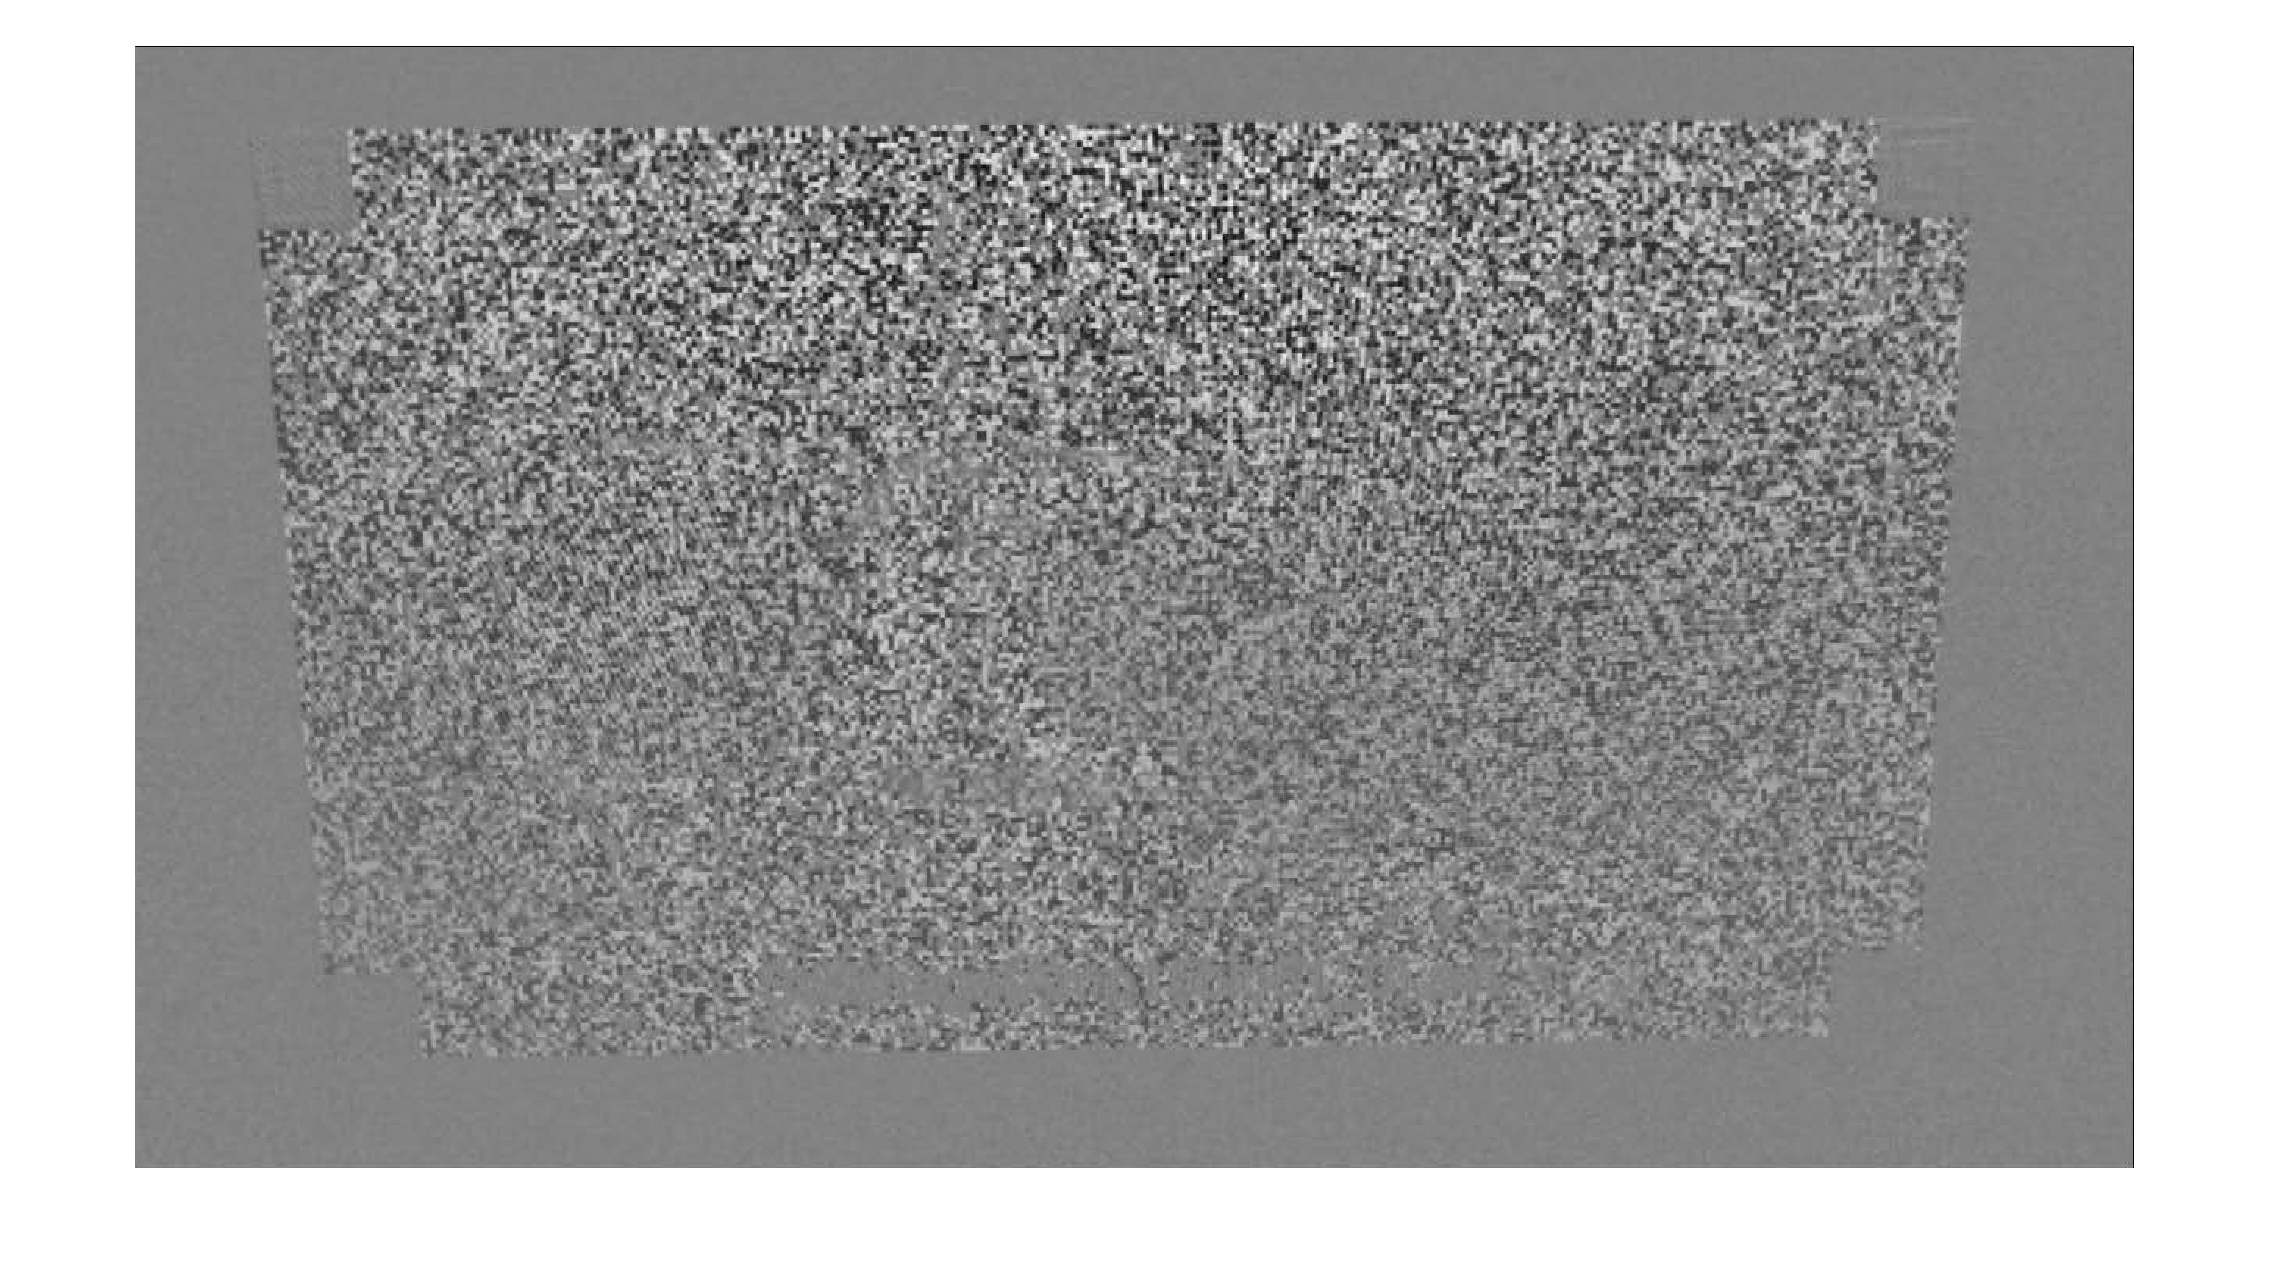
\includegraphics[scale=0.15]{images/4_ZweiteErfahrung/Differenzbild/5aufheben.pdf}\\

	\bottomrule
	\end{tabular}
\end{table} 


Offensichtlich ist die direkte Verwendung dieser Differenzbilder ein kniffliges Problem für die nächste Detektion. Um dieses Problem zu lösen, wurde ein Algorithmus zur Optimierung der Differenzbilder entwickelt.

Der Struktur eines QR Musters zeigt in Formel 4.29. Die äußerste "1" Schicht ist eine Trennmuster und die Zentralbereich bedeutet das QR Muster. Aufgrund der Modulationseigenschaften des \gls{david} Systems wird nur Element "1" nach Modulation offensichtlich verändert. Im Vergleich dazu werden die Element "0" nur klein verändert. Deswegen durch eine Absolutwertoperation, werden die QR Muster als Schwarz-Weiß-Schwarz-Weiß-Schwarz Ordnung darstellt. Dies ist die erwartende Modellstruktur, die in nächster Schritt operieren werden. Der detailliertes Operieren wird in Abschnitt "QR Muster Detektion" gegeben.

\begin{equation}
QR_{base} = \begin{bmatrix}
    1 &1 &1 &1 &1 &1 &1 &1 &1 \\
    1 &0 &0 &0 &0 &0 &0 &0 &1 \\
    1 &0 &1 &1 &1 &1 &1 &0 &1 \\ 
    1 &0 &1 &0 &0 &0 &1 &0 &1 \\ 
    1 &0 &1 &0 &0 &0 &1 &0 &1 \\ 
    1 &0 &1 &0 &0 &0 &1 &0 &1 \\ 
    1 &0 &1 &1 &1 &1 &1 &0 &1 \\ 
    1 &0 &0 &0 &0 &0 &0 &0 &1 \\ 
    1 &1 &1 &1 &1 &1 &1 &1 &1 \\ 
\end{bmatrix}
\end{equation}

Als nächstes werden ein Begriff $``Energie"$ vorstellen. Die auf numerischer Ebene bedeutet den Mittelwert der quadrierten Elemente des Bildes. Es ist bekannt sein, dass aufgrund der Subtraktion die Pixelwerte in das Gebiet, welches rund um die Modulationsbereich legt, gegeneinander aufgehoben werden. Deswegen in dieses Gebiet die Pixelwerte werden nur von Rausch beeinflusst und sehr klein sein werden. Im Vergleich dazu beträgt die Pixelwerte im Modulationbereich ein relativ größer Wert $\pm2A$, hier A beutet die Modulationsamplitude des Systems. Überlegen die Einfluss von Zeitsynchronisation, indem die Pixelwerte in einigem Teile der Modulationsbereich werden aufgrund Synchronisation auch ausgeglichen, nämlich die $``Energie"$ aufgehoben werden. Dann nehmen eine Regelmäßigkeit, die Größe der $``Energie"$ hängt hauptsächlich von die Pixelwerte im Modulationsbereich. Je größer die Pixelwerte sind, je höher der $``Energie"$ des Bildes ist, und je klarer das QR Muster werden. Gemäß dieser Regel berechnen die $``Energie"$ jedes Differenzbildes und anordnen in absteigender Reihenfolge. Um die folgende Detektion zu vereinfachen, fügen die ersten paar Bilder hinzu und erhalten einen zu detektierende Bilder. Die Praxis hat bewiesen, dass es ausreicht, die ersten drei Bilder zu nehmen.

Die Formel der $``Energie"$ wird in Gleichung 4.30 darstellt. Hier m,n repräsentiert die Anzahl der Zeilen und Spalten der Matrix. $diff(i,j)$ bedeutet die Pixelwert des Punkts in der m-ten Zeile die n-te Spalte der Matrix.

\begin{equation}
Energie = \frac{1}{m \times n} \sum_{i=1}^m \sum_{j=1}^n diff^2(i,j) \end{equation}

 

Hier in dieser Arbeit wird eine einfach Differenzbild Algorithmus vorstellen, wie folgen darstellt:

\begin{enumerate}
	\item Wähle zwei beliebige Bilder aus und subtrahiere, um Differenzbild zu enthalten.
	\item Nehmen eine Absolutoperation für jedes Differenzbild und berechnen dessen Energie. Um den Berechnungsaufwand zu reduzieren, kann nur der zentrale Bereich berechnet werden.
	\item Sortiere in absteigender Reihenfolge und nehmen die erste 3 Differenzbildern.
	\item Addieren diese 3 Differenzbildern, um eine detektierend Bild zu erhalten.
\end{enumerate}

Das Flussdiagramm wird in Abbildung gezeigt.
\begin{figure}[H]
 \centering 
 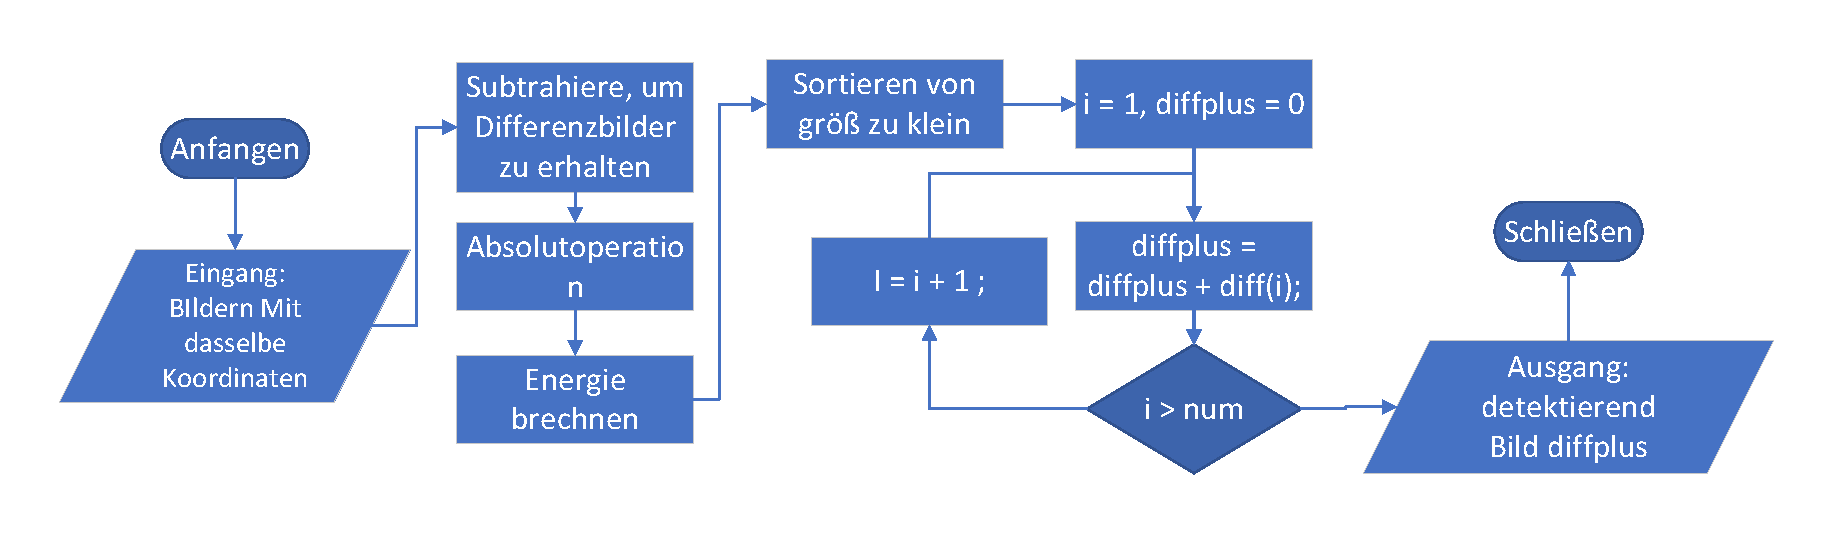
\includegraphics[keepaspectratio,width=0.9\textwidth]{images/4_ZweiteErfahrung/Differenzbild/Differenzbildflussigdiagramm.pdf}
 \caption{Differenzbild Flussigdiagramm}
 \label{fig:DifferenzbildFlussigdiagramm}
\end{figure} 

Eine Beispiel für detektierendes Bild wird in Abbildung 4.18 gezeigt. Durch die Optimierung kann die QR Muster an der Eck des Bildes einfachen detektiert werden.

\begin{figure}[H]
 \centering 
 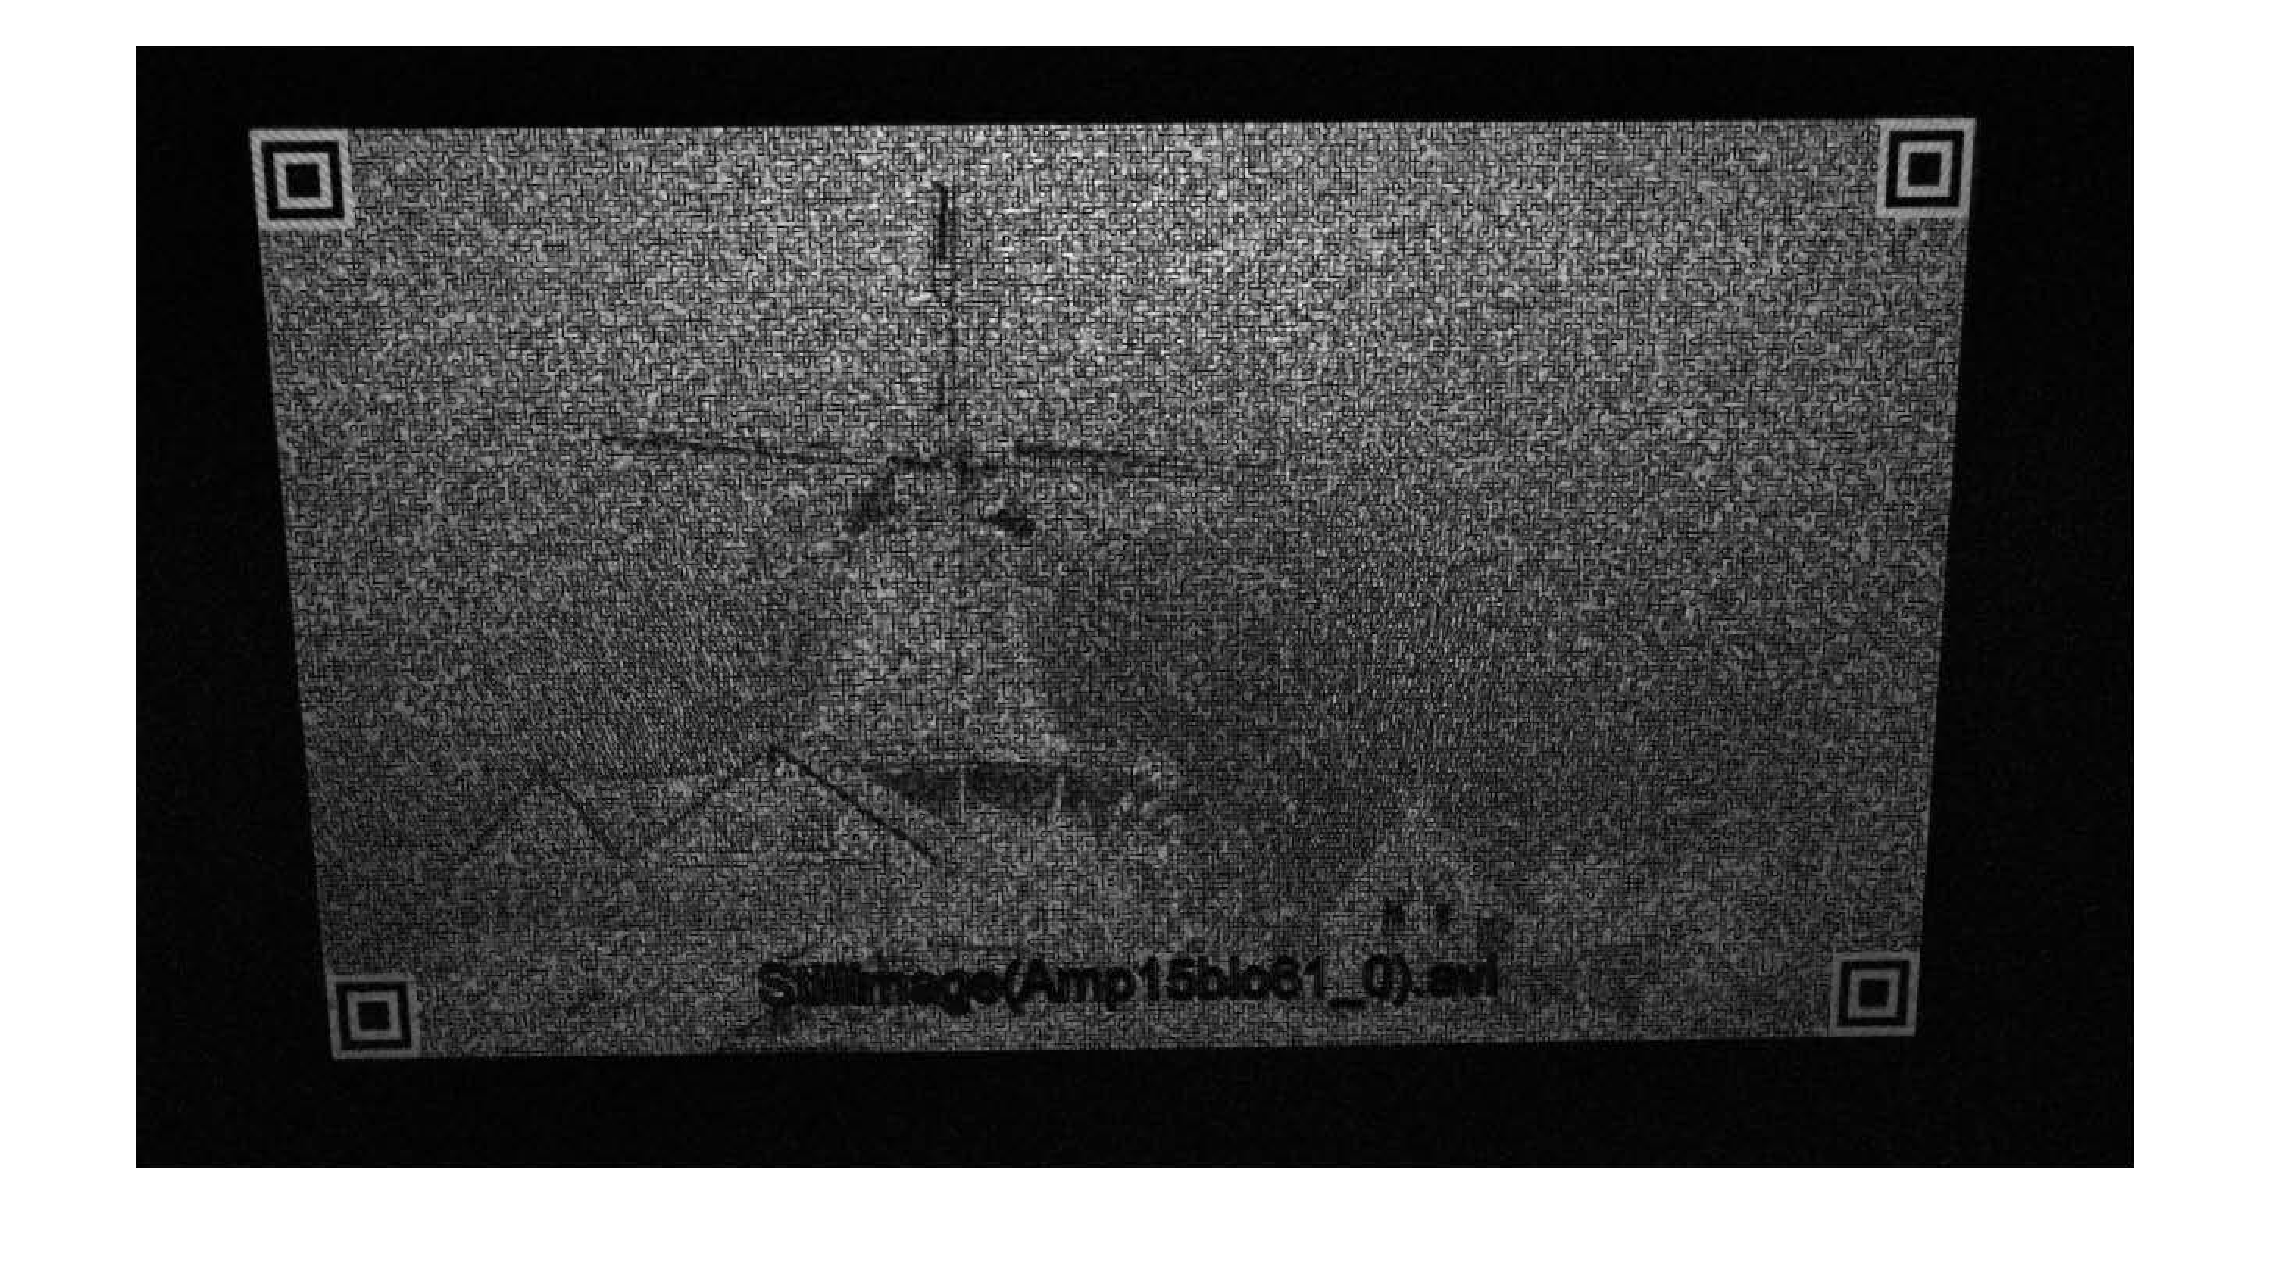
\includegraphics[keepaspectratio,width=0.8\textwidth]{images/4_ZweiteErfahrung/Differenzbild/diffplus.pdf}
 \caption{Differenzbild Beispiel}
 \label{fig:Differenzbild}
\end{figure} 


\section{Bildverarbeitung} 
Durch die Differnzbild Optimierung, wird ein detektierendes Bild enthältet. Es ist noch ein Graustufenbild und muss noch einige Bildverarbeitung nehmen. Dadurch können kleine Punkte und Lücken, die durch Rauschen und Fehler verursacht werden, entfernt werden, um die nachfolgende Detektion zu erleichtern. Der detailliert Inhalt der Bildverarbeitung wurde in der anderen Methode eingeführt, hier ist nur eine kurze Beschreibung der verwendeten Funktionen in Matlab. 

\textbf{Bild Binarisierung}

Für die Schwellenwertbildung und das Erstellen eines Binärbildes wurde eine Funktion namens "imbinarize" verwenden. Diese Funktion erhält das Bild und verwendet ein anpassungsfähige Schwellwert, um das Schwarz-Weiß-Bild zurückzugeben. Das ist genug für QR-Pattern Detktion, weil es nur dunkle und helle Module enthält, die binär 1 bzw. 0 sind. 

\textbf{Medianfilter}

Der Grund für das Median-Filtern ist, dass manchmal beim Prozess Binarisierung aus einem Bild die Muster wie Salz- und Pfeffergeräusche erzeugt werden können. Um diesen Fehler zu vermeiden, ist Median Filterung eine leistungsfähig Methode. Das Skript ist so einfach wie medfilt2(img). Zur Verbesserung der Ergebnisse kann natürlich die verschiedenen Fenstergrößen für die Matlab-Funktion verwenden.

\textbf{Morphologie}

Mit öffnenden und schließenden Filtern können die Lücken zwischen Blöcken und die kleine Punkte von Rausch stark reduziert werden, was das resultierende binär Bild zu einer guten Schätzung des QR-Pattern macht. 

\section{QR Musters Detektion} 

Nach Bildverarbeitung wird nun die QR Musters Detektion ausgeführt. Die Ziel einer QR Musters Detektion ist die Zentrum des Musters im Bild zu lokalisieren und dadurch die Bild zu rekonstruieren. Abbildung 4.20 zeigt eine geometrische Struktur des QR Musters. An jedem Ecke der Modulartionsbereiche gibt es eine solche QR Muster.

\begin{figure}[H]
 \centering 
 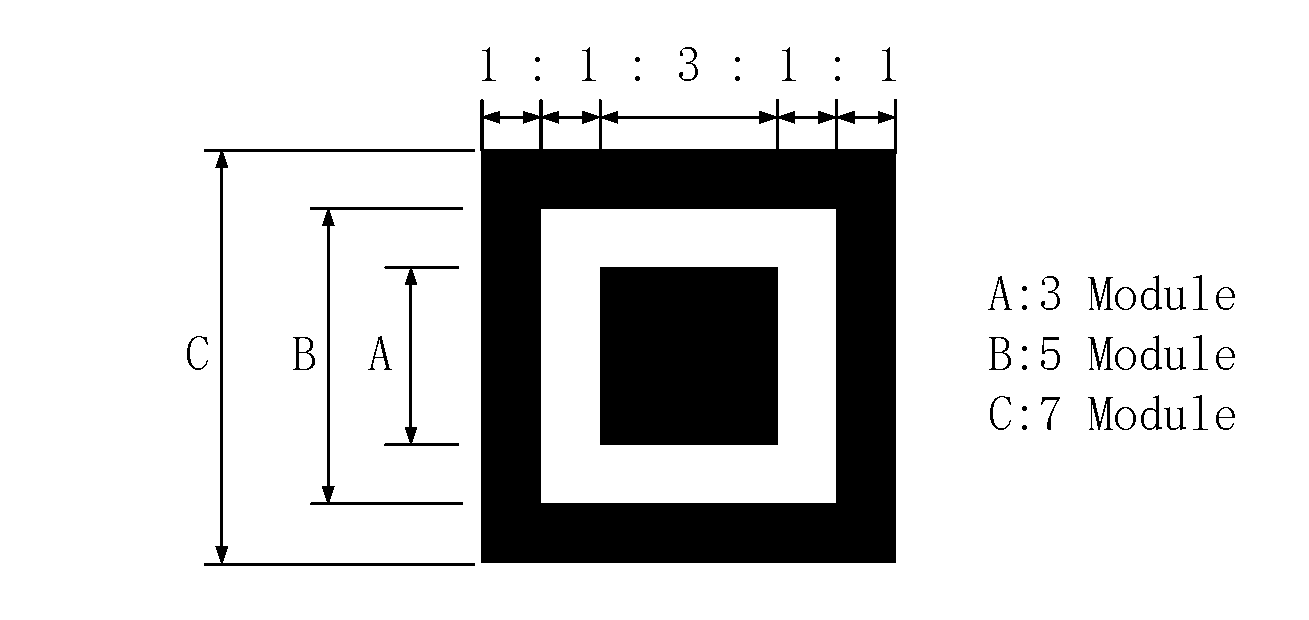
\includegraphics[keepaspectratio,width=0.9\textwidth]{images/4_ZweiteErfahrung/QRMuster/QRPattern.pdf}
 \caption{QR Pattern}
 \label{fig:QRPattern}
\end{figure}

Aus der geometrischen Sicht kann jedes Muster als drei konzentrische Quadrate betrachtet werden und besteht aus eine schwarzen (dunklen) $7 \times 7$ Modulen, eine weißen (hellen) $5 \times 5$ Modulen und schließlich eine dunklen $3 \times 3$ Modulen. Von Kenntnisse der Geometrie können bekannt sein, in jeder Richtung das Breiteverhältnis der alternativen Schwarz- und Weißmodul in einem Muster eine Bieziehnung $1:1:3:1:1$ beträgt, wie es in Abbildung 4.21 zeigt. Diese wichtige Eigenschaft hilft uns, die Lokalität der QR Muster zu finden. In der Praxis rund um die Muster gibt es noch ein Trennmuster, das ein Funktionsmuster mit aller weißen (hellen) Module(Breit ein Modul). Es spielt eine Rolle als eine Grenze zwischen den Mustern und dem Datenbereich, um die Verwechslungen zwischen Muster und Daten zu vermeiden.
 
 \begin{figure}[H]
 \centering 
 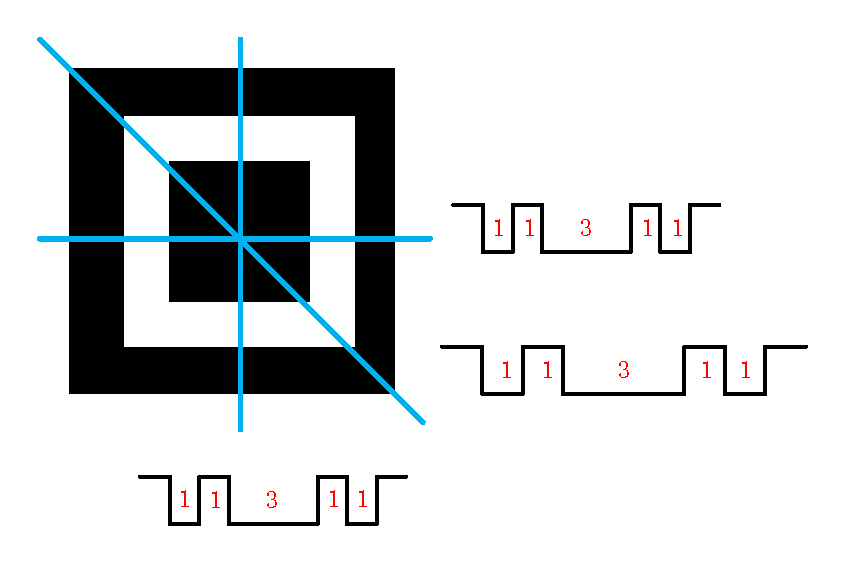
\includegraphics[keepaspectratio,width=0.7\textwidth]{images/4_ZweiteErfahrung/QRMuster/QP_Patternratio.pdf}
 \caption{QR Pattern Ratio}
 \label{fig:QRPatternRatio}
\end{figure}

Als nächstes werden die detaillierten Schritte der Detektion eingeführt und es wird mit Funktion "detectFIP" in Matlab implementiert.

\textbf{Schritt 1:}

Zuerst überlegen die größe Berechnungsaufwand für die Analysen des ganzen  Bilds, teilen einige kleine Bereiche auf, die QR Muster enthalten können.

\textbf{Schritt 2:}

Scannen jede Zeile dieses kleinen Bereiches und speichern die Länge der Schwarz und Weiß Module in eine fünf Element Vektor. Die Länge der Module heißt die Anzahl aufeinanderfolgende Pixel in einer Zeile mit die gleiche Farbe. Speicherreihenfolge in diesem Vektor ist laut Schwarz-Weiß-Schwarz-Weiß-Schwarz. Es sollte hier angemerkt werden, dass das erste Element des Vektors die Anzahl der schwarzen Module enthält. 

\textbf{Schritt 3:}

Immer wenn das fünfte Element des Vektors gezählt wird, nehmen die fünf Elemente und ein Urteil machen, ob die Beziehung der Zählungen nahe genug an den $1:1:3:1:1$ Verhältnissen ist. Wenn die Bedingung erfüllt ist, gehen zum nächsten Schritt. Dagegen verschieben den Vektor um zwei nach links und werfen die ersten und zweiten Elemente des Vektors weg. AnschliSeßen gehen zurück zu Schritt 2, um weiter Scannen und Zählen zu beginnen.                

\textbf{Schritt 4:}

Verarbeiten die Elemente vom Vektor, um das ungefähre horizontale Zentrum zu erhalten. Mache eine Kreuzprüfung an diesem Punkt, welche besteht aus den Schritten 2 und 3, der Unterschied dazwichen wird der horizontale Scan durch einen vertikalen Scan ersetzt. Anschließen machen ein Urteil, ob eine vertikale Zentrum gefunden ist. Wenn Ja bestimmt, machen eine Kreuz-Kreuzprüfung mit horizontale Scan, um die Ergebnis zu optimieren. Dies wird hauptsächlich benötigt, um die reale horizontale Mitte des Musters in  extremer Schräglage Fällen zu lokalisieren. Speichern der potenzielle Zetrum, danach leeren die Elemente des Vektors und wieder zu zweiten Schritt, um einen neuen Scan machen. Ansonsten verschieben den Vektor um zwei nach links und werfen die ersten und zweiten Elemente des Vektors weg. Gehen zurück zu Schritt 2, um weiter Scannen und Zählen zu beginnen.                

\textbf{Schritt 5:}

Verarbeiten die Ausgabe des vorherigen Schritts, falls es nicht nur eine potentiell Muster Zentrum gefunden, nutzen einen "selectBestPattern", um die beste zu auswählen. Es sollte angemerkt werden, dass wenn die mögliche Muster nach dem Ende der Erkundung nicht gefunden wird, ein spezielle Signal zurückgegeben wird und die System zu Schritt Differenzbild Optimierung zurückkehren wird. Die Operation besteht darin, der ursprünglichen Bild, die aus drei Differenzbild besteht, ein mehre Differenzbild hinzuzufügen.
                       
\textbf{Schritt 6:}

Durch die gefunden Muster Zentren, machen eine projective Transformation, un die Ecke des Bildes zu bestimmen.


Die folgende Abbildung 4.22 zeigt die Flussdiagramm einer Detektion für QR Muster.

\begin{figure}[H]
 \centering 
 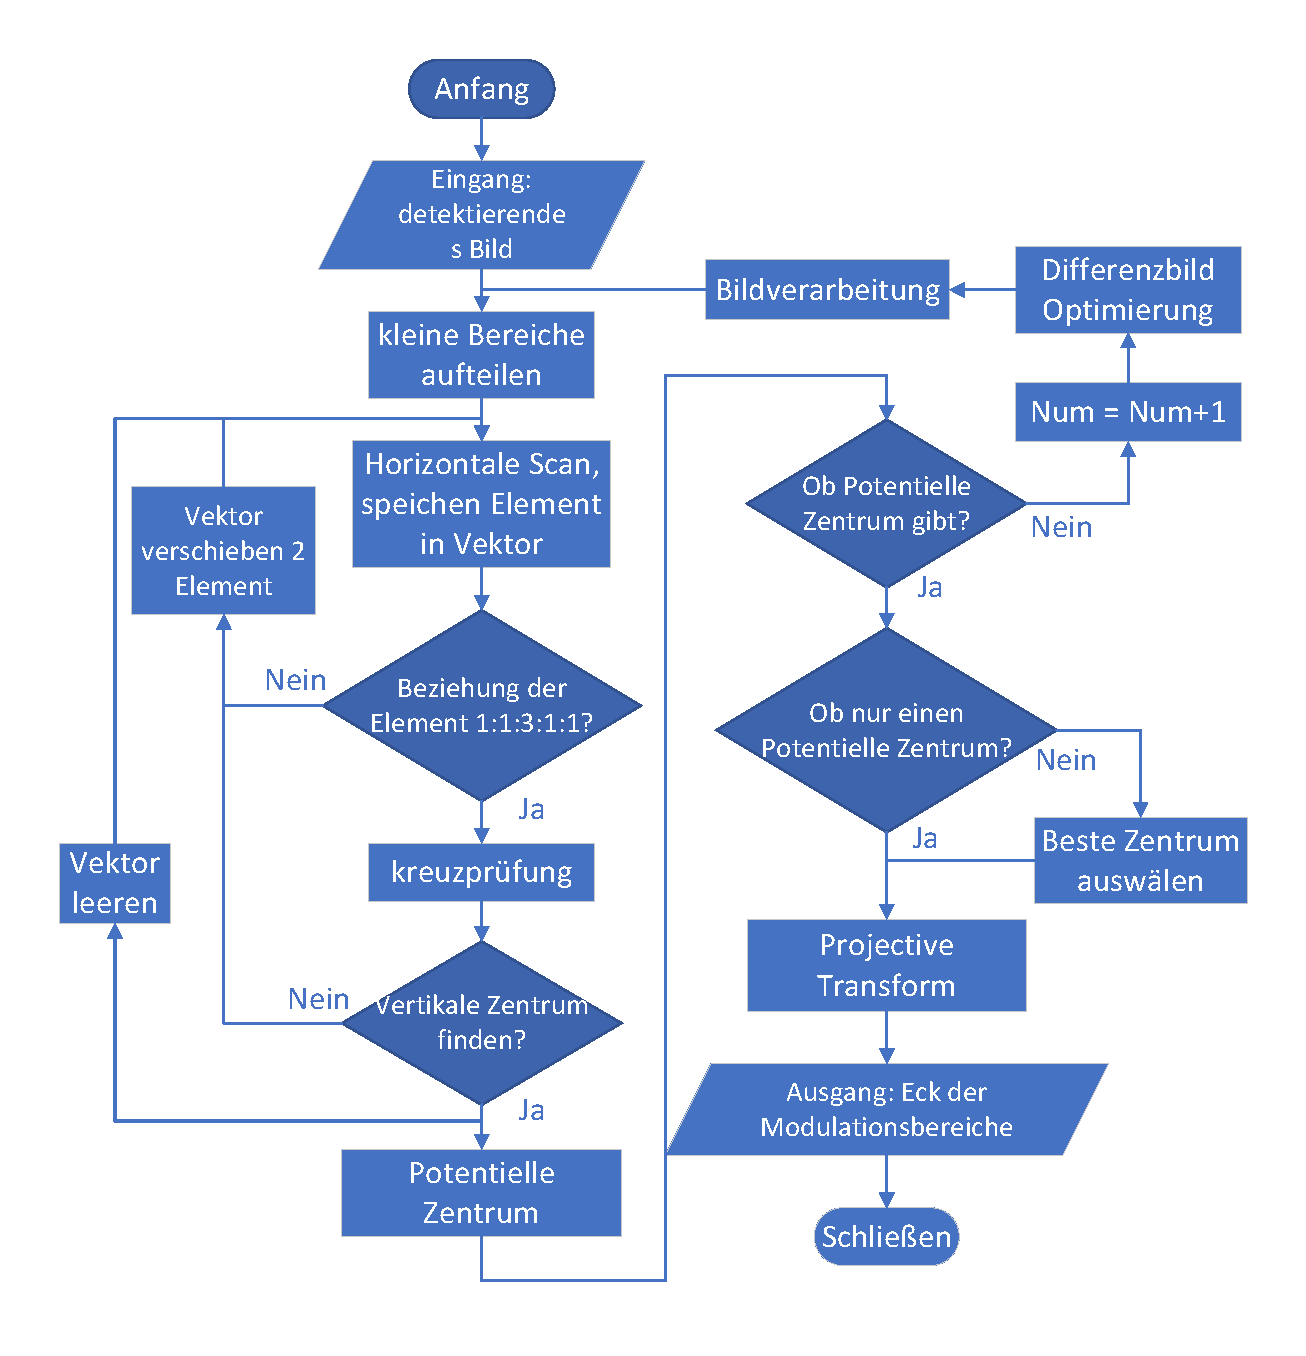
\includegraphics[keepaspectratio,width=1.0\textwidth]{images/4_ZweiteErfahrung/QRMuster/QR_flussdiagramm.pdf}
 \caption{Flussdiagramm der QR Muster Detektion}
 \label{fig:Flussdiagramm der Methode}
\end{figure}

Einige Beipiel für QR Muster Detektion zeigt in Abbildung:

\chapter{Auswertung} \label{cha:Auswertung}

Text hier zwischen. Referenz auf ein Bild mit cleverref (siehe \cref{fig:mathplot}). Und dann noch ein paar Zitierungen \cite{Reinhold:2013fk,Moon,IEEE2011}.

\section{Section}

Jetzt nur noch schreiben! :)



\chapter{Zusammenfassung} \label{cha:Zusammenfassung}

In dieser Arbeit werden zwei Verfahren zur Ausschnittsdetektion für die Screen-Camera Visible Light Communication untersucht und implementiert. Methode 1 ist vom differentiellen Modulationsverfahren des David-Systems inspiriert. d.h. Daten werden mit geringer Amplitude im Videosignal differentiell überlagert. In der Methode wird ein QR Muster an jeder Ecke der Datenebene hinzugefügt und dann mit den Daten zusammen hinter dem Bild moduliert. Diese Methode kann nicht nur den unschönen Effekt lösen, welcher durch direktes Hinzufügen des QR Musters zu dem Videobild verursacht wird, sondern kann auch den QR Muster durch seine spezifische geometrische Eigenschaft, d.h. in jeder Richtung beträgt das Breiteverhältnis $1:1:3:1:1$, effektiv erkennen. Dadurch wird schließlich der Modulationsbereich bestimmt. Das 2. Verfahren wird in den physikalischen Eigenschaften des Modulationsbereichs ausgeführt. Im \gls{david} System wirkt der Bildschirm als Übertragungsende, und der Bildschirmbereich ist der Modulationsbereich, der im Allgemeinen in Form eines Rechtecks ist. Dadurch kann dieses Problem in eine rechteckige Erkennung umgewandelt werden. Durch die Radon Transformation wird die längste gerade Linie in dem Bild detektiert, um ein Rechteck bzw. den Modulationsbereich, zu bestimmen.

zwei Aufnahmebedingungen wurden in dieser Arbeit berücksichtigt, eine ist die Aufnahme mit dem Smartphone aus der Hand und die andere auf einem Stativ. Handheld-Kamera-Shooting ist eine der häufigsten und bequemsten Aufnahmemethoden im Alltag, und hat eine unerlässliche Position in der praktischen Anwendung. Zu diesem Zweck wurde ein Bildregistrierungsmodul speziell für Handschütteln entwickelt, welche Merkmals Detektion, \gls{ransac}, Kamera Modell und Nichtlineare Optimierung beinhaltet. Beim Testen beträgt die relative Verschiebung zwischen den entsprechenden Punkten des korrigierten Bildes c.a. 0.3 Pixel. Dies führt zu einem relativ guten Differenzbild. Dieser spielte eine wichtige Rolle weil beide Verfahren in dieser Arbeit auf der Detektion von Differenzbildern basieren. Dafür wird der Begriff $ ``Energie" $ eingeführt, welcher die Klarheit des Modulationsbereichs repräsentiert. Gemäß der Energiesortierung werden die klarsten Bilder ausgewählt und hinzugefügt, um das zu detektierende Bild zu erhalten. In Methode 1 werden die beide obigen Schritte implementiert, und durch Auswertung die durchschnittliche Abweichung ca. $ 1-2 $ Pixel bemessen. Es sollte hier angemerkt werden, dass aufgrund der Eigenschaften der Bildregistrierung das Video, das in Methode 1 aufgenommen wurde, ein statisches Video ist, d.h. der Inhalt des Videos hat sich nicht geändert. Der Grund dafür ist, dass der Punkt der Merkmals Detektion hauptsächlich auf dem Inhalt des Videos basiert. Wenn sich der Videoinhalt stark ändert, ist es schwierig, die Genauigkeit der Bildwiederherstellung zu garantieren. Einige bei der Arbeit versuchten Methoden war die Abschirmung des zentralen Bereichs während der Merkmals Detektion, d.h. nur die Merkmale in der Umgebung des Bildes wurden erkannt, was nicht zufriedenstellend ist. Methode 2 implementiert die Erkennung des Modulationsbereichs unter Verwendung eines Stativs. Nach der Erkennung beträgt die durchschnittliche Abweichung ebenfalls ca. $ 1-2 $ Pixel. In beiden Methoden kann der Modulationsbereich mit Parametern, wie die Modulationsapmlitude als 4,  der Datenblock als $ 4 \times 4 Pixel$, erfolgreich bestimmt werden. 

Für dieses Thema gibt es einige mögliche weitere Forschung in der Zukunft. Zuerst kann wie oben erwähnt, ein Verfahren gefunden werden, welches beim Aufnehmen des dynamischen Videos mit dem Smartphone aus der Hand, das Handschütteln-Problem effektiv löst. Der Fokus liegt darauf, die Wirkung vom Video-Inhalt zu neutralisieren und das Bild nur auf die Merkmale des Hintergrunds zu filtern. Zweitens, die in dieser Arbeit verwendete Differenzbild Optimierungsmethode, kann aufgrund der Berechnung der $ ``Energie" $ für jedes Differenzbild zu einer großen Rechenlast führen. Ein effektives Verfahren wäre versuchen, ein zu detektierendes Bild, das auf dem bekannten Differenzbild basiert, effizient zu generieren. Schließlich wurde in Experiment festgestellt, dass unter denselben Parametern die Verwendung des gleichen Smartphones mit dem gleichen Video-Inhalt auf verschiedenen Bildschirmen, zu unterschiedlichen Ergebnissen führt. Dadurch können die Auswirkungen der Bildschirmfaktoren, wie z.B. Beleuchtungsart, Auflösung, Bildwiederholfrequenz, weiter erforscht werden.






\appendix
\chapter{Erster Anhang} \label{cha:anhangA}

\section{Section}

Jetzt nur noch schreiben! :)




\backmatter
\cleardoublepage
% \chapter*{Nomenklatur} \addcontentsline{toc}{chapter}{Nomenklatur}
% \markboth{Nomenklatur}{Nomenklatur}

\printglossary[type=\acronymtype, style=tab_style] %[toctitle=Symbolverzeichnis,title=Symbolverzeichnis] 
\printglossary[type=symbol, style=tab_style_sym]
% \printglossary

\listoffigures%				Abbildungsverzeichnis
\listoftables%				Tabellenverzeichnis
\lstlistoflistings%			Listingsverzeichnis

% \nocite{*}%				es wird alles zitiert
\printbibliography%			Literaturverzeichnis

\makeatletter
\cleardoublepage
\thispagestyle{empty}
\onehalfspacing
\LARGE
\begin{center}
	\textbf{Eidesstattliche Versicherung}
\end{center}

\small
\vspace{\baselineskip}
\underline{\makebox[.4\textwidth][c]{\@authorsurname,\space\@authorfirstname}}
\hspace{.25\textwidth}
\underline{\makebox[.3\textwidth][c]{\@matrikelnumber}}
\newline
\makebox[.4\textwidth][l]{Name, Vorname}
\hspace{.25\textwidth}
\makebox[.3\textwidth][l]{Matr.-Nr.}

Ich versichere hiermit an Eides statt, dass ich die vorliegende \@documenttype\space mit dem Titel

\underline{\makebox[0.97\textwidth][c]{\@thesistitle}}

selbstständig und ohne unzulässige fremde Hilfe erbracht habe. Ich habe keine anderen als die 
angegebenen Quellen und Hilfsmittel benutzt sowie wörtliche und sinngemäße Zitate kenntlich 
gemacht. Die Arbeit hat in gleicher oder ähnlicher Form noch keiner Prü\-fungs\-be\-hörde 
vorgelegen. 
\vspace{\baselineskip}

\underline{\makebox[.4\textwidth][c]{Dortmund, \today}}
\hspace{.25\textwidth}
\underline{\hspace{.3\textwidth}}
\newline
\makebox[.4\textwidth][l]{Ort, Datum}
\hspace{.25\textwidth}
\makebox[.3\textwidth][l]{Unterschrift}

\vspace{\baselineskip}

\textbf{Belehrung}: 

Wer vorsätzlich gegen eine die Täuschung über Prüfungsleistungen betreffende Regelung einer 
Hochschulprüfungsordnung verstößt, handelt ordnungswidrig. Die Ordnungswidrigkeit kann mit 
einer Geldbuße von bis zu 50.000,00\,€ geahndet werden. Zuständige Verwaltungs\-behörde für 
die Verfolgung und Ahndung von Ordnungswidrigkeiten ist der Kanzler/die Kanzlerin der 
Technischen Universität Dortmund. Im Falle eines mehrfachen oder sonstigen schwerwiegenden 
Täuschungs\-versuches kann der Prüfling zudem exmatrikuliert werden. (§ 63 Abs. 5 
Hochschulgesetz - HG - )  

Die Abgabe einer falschen Versicherung an Eides statt wird mit Freiheitsstrafe bis zu 3 Jahren 
oder mit Geldstrafe bestraft.  

Die Technische Universität Dortmund wird ggf. elektronische Vergleichswerkzeuge (wie z.B. die 
Software „turnitin“) zur Überprüfung von Ordnungswidrigkeiten in Prüfungsverfahren nutzen. 

Die oben stehende Belehrung habe ich zur Kenntnis genommen: 
\vspace{\baselineskip}

\underline{\makebox[.4\textwidth][c]{Dortmund, \today}}
\hspace{.25\textwidth}
\underline{\hspace{.3\textwidth}}
\newline
\makebox[.4\textwidth][l]{Ort, Datum}
\hspace{.25\textwidth}
\makebox[.3\textwidth][l]{Unterschrift}
\makeatother
\end{document}